\documentclass[12pt,a4paper,openany]{abntex2}
% openany - para eliminar paginas em branco, que surgem pois os capitulos so comecam em paginas impares no modo frente e verso
\usepackage[utf8]{inputenc}
\usepackage{amsmath}
\usepackage{esint}
\usepackage{amsfonts}
\usepackage{amssymb}
\usepackage{graphicx}
\usepackage{subfig}
\graphicspath{{fig/}}
\providecommand{\norm}[1]{\lVert#1\rVert}
\usepackage{empheq}
\usepackage{lscape}

%\usepackage[alf ,abnt-etal-cite=2 , abnt-year-extra-label=yes , abnt-etal-list=0, abnt-etal-text=it]{abntex2cite}
%instalar abntcite.sty

\begin{document}

\tableofcontents

\chapter{Introdu\c{c}\~ao}
Como podemos constatar em \cite{eringen_1963}, existe uma similaridade matem\'tica entre a propaga\c{c}\~ao de ondas eletromagn\'eticas e el\'asticas em camadas que comp\~oem a subsuperf\'icie terrestre, que faz com que todas essas ondas tridimensionais possam ser representadas por equa\c{c}\~oes que possuem as mesmas propriedades. Verificamos tamb\'em que \'e poss\'ivel realizar o acoplamento dessas ondas, dentro de uma teoria conhecida como \textit{magnetoelasticidade}. Assim, segundo \cite{Ursin-1983}, podemos aplicar a mesma abordagem para tratamento tanto de ondas ac\'usticas como de ondas eletromagn\'eticas, e esse trabalho visa fazer o levantamento te\'orico de tal aplica\c{c}\~ao. A abordagem consiste basicamente em usar as tranformadas de Fourier, Laplace e Bessel no sistema de equa\c{c}\~oes diferenciais parciais que descrevem o acoplamento magnetoel\'astico, escrevendo-o em fun\c{c}\~ao da frequ\^encia temporal e numa forma matricial. Atrav\'es de transforma\c{c}\~ao das coordenadas laterais, o sistema \'e deixado em fun\c{c}\~ao apenas da profundidade e o sistema inical de EDP's \'e transformado em dois sistemas de equa\c{c}\~oes diferenciais ordin\'arias onde cada grandeza pode ser claculada separadamente. Tal procedimento \'e denominado \textit{m\'etodo matricial}.

Alguns pesquisadores j\'a utilizaram o m\'etodo matricial em sistema acoplados. \cite{White_Zhou_2006} utilizaram em m\'etodos de \textit{Eletros\'ismica} que estuda a convers\~ao de ondas eletromagn\'eticas em ondas s\'ismicas na subsuperf\'icie terrestre na prospec\c{c}\~ao de hidrocarbonetos. A convers\~ao entre as ondas ocorre em meios porosos onde uma onda eletromagn\'etica pode excitar uma onda s\'ismica de mesma frequ\^encia e vice-versa, atrav\'es do movimento dos fluidos contidos nos poros. A altera\c{c}\~ao que uma onda eletromagn\'etica promove numa onda s\'ismica de mesma frequ\^encia pode ser registrada na superf\'icie terrestre trazendo informa\c{c}\~oes sobre as propriedades el\'etricas da subsuperf\'icie. 

\cite{Azeredo_2013} aplica o m\'etodo matricial para resolver de forma anal\'itico-num\'erica equa\c{c}\~oes de poroelasticidade que descrevem a propaga\c{c}\~ao de ondas em meio plano estratificado formado por camadas homog\^eneas e isotr\'opicas. O m\'etodo fornece f\'ormulas expl\'icitas para a constru\c{c}\~ao de algoritmo computacional  para obter a solu\c{c}\~ao do problema.
\chapter{Revis\~ao Bibliogr\'afica}

Existem diferentes tipos de modelos f\'isicos que descrevem as propaga\c{c}\~oes de ondas el\'asticas e eletromagn\'eticas bem como a intera\c{c}\~oes entre elas na subsuperf\'icie terrestre. A esses modelos s\~ao aplicados variados m\'etodos matem\'aticos e num\'ericos, incluindo o m\'etodo matricial, que realizam a simula\c{c}\~ao desses fen\^omenos f\'isicos. Apresentaremos nesse cap\'itulo algumas publica\c{c}\~oes nesse sentido, as quais est\~ao de alguma forma relacionadas ao objetivo desta monografia. 

\section{Prospec\c{c}\~ao Eletro-s\'ismica}

Alguns pesquisadores j\'a trabalharam em sistema acoplados, como \cite{White_Zhou_2006}, que estudaram fen\^omenos de \textit{Eletro-s\'ismica} que descrevem a convers\~ao de ondas eletromagn\'eticas em ondas s\'ismicas na subsuperf\'icie terrestre na prospec\c{c}\~ao de hidrocarbonetos. A convers\~ao entre as ondas ocorre em meios porosos onde uma onda eletromagn\'etica pode excitar uma onda s\'ismica de mesma frequ\^encia e vice-versa, atrav\'es do movimento dos fluidos contidos nos poros. A altera\c{c}\~ao que uma onda eletromagn\'etica promove numa onda s\'ismica de mesma frequ\^encia pode ser registrada na superf\'icie terrestre trazendo informa\c{c}\~oes sobre as propriedades el\'etricas da subsuperf\'icie. 


Esses estudiosos aplicam transformadas nas EDP's deduzidas por \cite{pride_94}, as quais passam a ser escritas como sistemas de EDO's. Utilizam o m\'etodo matricial contido em \cite{Ursin-1983} nessas EDO's para obter as solu\c{c}\~oes em cada camada estratigr\'afica e, por \'ultimo, retornam as solu\c{c}\~oes para o espa\c{c}o original. Ap\'os deduzir f\'ormulas explicitas, apresentam um algoritmo computacional onde os resultados num\'ericos s\~ao obtidos. Esse algoritmo pode ser modificado para computar separadamente a propaga\c{c}\~ao de ondas el\'asticas, ondas eletromagn\'eticas e as ondas da teoria de Biot. Como o artigo trata da produ\c{c}\~ao de onda s\'ismica atrav\'es de fontes eletromagn\'eticas, \'e necess\'ario um n\'ivel suficiente de corrente el\'etrica para que se produza uma resposta s\'ismica satisfat\'oria. 


Na figura \ref{fig.white_zhou} podemos observar um tra\c{c}o s\'ismico de fonte eletromagn\'etica obitdo pelo simulador, que \'e an\'alogo a um tra\c{c}o s\'ismico convencional. Note pela escala da figura que sinais muito pequenos podem ser identificados. Esses pequenos sinais t\^em no m\'aximo a amplitude dos ru\'idos provocados pela sensibilidade dos geofones e s\~ao menores do que muitas fontes de ru\'idos que podem ser identificadas no campos, da\'i uma m\'edia consider\'avel de sinais se faz necess\'aria para que a detec\c{c}\~ao seja plenamente confi\'avel. Como as equa\c{c}\~oes que descrevem os fen\^omenos s\~ao linearizadas, as escalas dos resultados tamb\'em s\~ao lineares com as correntes el\'etricas usadas como fonte, ent\~ao as pequenas respostas podem ser melhoradas com o aumento da corrente.
\begin{figure}
\centering
\includegraphics[scale=1]{white_zhou}
\caption{\textit{Tra\c{c}o s\'ismico obtido a partir de for\c{c}as eletromagn\'eticas como fonte.}}
\label{fig.white_zhou}
\end{figure}  

\section{M\'etodo Matricial em Meios Poroel\'asticos}\label{sec.matricial_poroelast}


\subsection{Sistema de Biot para Baixas Frequ\^encias}\label{sec.biot}

Alguns pesquisadores utilizaram o m\'etodo matricial em meios poroel\'asticos. Por exemplo,
\cite{Azeredo_2013} aplica o m\'etodo matricial para resolver de forma anal\'itico-num\'erica equa\c{c}\~oes de poroelasticidade deduzidas por Maurice Biot em 1956, as quais descrevem a propaga\c{c}\~ao de ondas em meio plano estratificado formado por camadas homog\^eneas e isotr\'opicas. 


Este trabalho apresenta dois tipos de fontes para produ\c{c}\~ao de ondas s\'ismicas:  uma fonte constitu\'ida por dinamite e uma fonte que emite uma for\c{c}a pontual vertical, que pode ser tipo martelo, queda de peso ou \textit{vibroseis}. O m\'etodo fornece f\'ormulas expl\'icitas para a constru\c{c}\~ao de algoritmo computacional  para obter a solu\c{c}\~ao do problema considerando que o fluxo de fluido \'e do tipo \textit{Poiseuille}, isto \'e, baixo n\'umero de \textit{Reynolds} e baixas frequ\^encias.

S\~ao apresentados alguns modelos geol\'ogicos para realiza\c{c}\~ao das simula\c{c}\~oes num\'ericas e cada modelo \'e testado utilizando diferentes frequ\^encias. Um desses modelos apresenta duas camadas horizontais homog\^eneas e isotr\'opicas com a interface terra-ar localizada em $z_0=0\,m$  e a superf\'icie de descontinuidade \'e dada na profundidade $z_1=1500\,m$. Al\'em disso,
considera-se que a camada 2 tem espessura infinita e a frequ\^encia de propaga\c{c}\~ao das ondas \'e de $15\,Hz$. Podemos visualizar na figura \ref{fig.marcia} o surgimento de dois eventos: o evento 1 representa a onda direta, a qual atinge o receptor sem que haja reflex\~ao em qualquer interface, e o segundo evento \'e a onda refletida na interface de descontinuidade entre a primeira e segunda camadas. S\~ao apresentados dois gr\'aficos simulando diferentes dist\^ancias entre fonte e receptor, pois assim \'e poss\'ivel analisar sua influ\^encia na amplitude do sinal registrado.
\begin{figure}
\centering
\includegraphics[scale=.77]{simograma_marcia}
\caption{\textit{Componente vertical da velocidade da matriz porosa. Frequ\^encia dominante da fonte igual a $15\,Hz$ e dist\^ancia fonte-receptor igual a: (a) $500\,m$ e (b) $1000\,m$.}}
\label{fig.marcia}
\end{figure}


Sendo assim, observa-se que, \`a medida em que a dist\^ancia fonte-receptor aumenta, passando de $500\,m$ para $1000\,m$, a amplitude do sinal registrado diminui. Isto acontece porque a amplitude da onda s\'ismica diminui com o passar do tempo devido \`a redistribui\c{c}\~ao da energia entre as fases durante da passagem da onda s\'ismica atrav\'es de meio poroso. 
%Observe que, como esse modelo \'e composto por apenas uma superf\'icie de descontinuidade, aparecem apenas os eventos 1 e 2.

\subsection{Propaga\c{c}\~ao para Altas Frequ\^encias e Sistema de Biot-JKD}\label{sec.biot-jkd}

Outro exemplo de propaga\c{c}\~ao de ondas em meios poroel\'asticos pode ser visto em \cite{miranda_2016}, que utliza o modelo de Biot-JKD em regime de altas frequ\^encias. Em 1987, Johnson, Koplik e Desher (JKD) publicaram uma express\~ao geral da permeabilidade din\^amica, a qual varia de acordo com a frequ\^encia temporal, para caracterizar a dispers\~ao de energia no caso de poros aleat\'orios. Para baixas frequ\^encias, o comprimento de onda \'e grande quando comparado com a dimens\~ao do volume elementar: os efeitos viscosos s\~ao
preponderantes. J\'a no caso de altas frequ\^encias, o comprimento de onda \'e compar\'avel com a dimens\~ao do volume elementar: os efeitos inerciais s\~ao preponderantes. O limite entre baixas e altas frequ\^encias \'e atingido quando os efeitos viscosos e inerciais s\~ao similares.

O trabalho apresenta uma an\'alise dos efeitos de dispers\~ao e atenua\c{c}\~ao das ondas, fazendo uma compara\c{c}\~ao entre os modelos de Biot e Biot-JKD. Na figura \ref{fig.dispersao_mari}, podemos observar um gr\'afico mostrando as velocidades de fase para ambos os modelos em fun\c{c}\~ao da frequ\^encia temporal.
\begin{figure}
\centering
\includegraphics[scale=.8]{dispersao_mari}
\caption{\textit{Velocidades de fase em fun\c{c}\~ao da frequ\^encia.}}
\label{fig.dispersao_mari}
\end{figure} 
Para baixas frequ\^encias, as curvas de dispers\~ao tem valores aproximados. Para o intervalo $[10^4,10^6]\,Hz$, as curvas apresentam uma diferen\c{c}a significativa e para frequ\^encias maiores que $10^6\,Hz$, ambas as velocidades se aproximam do valor $1370\,m/s$.


Na figura \ref{fig.atenuacao_mari}, podemos observar um gr\'afico comparando as atenua\c{c}\~oes para os modelos de Biot e Biot-JKD tamb\'em em fun\c{c}\~ao da frequ\^encia temporal.
\begin{figure}
\centering
\includegraphics[scale=.78]{atenuacao_mari}
\caption{\textit{Atenua\c{c}\~ao em fun\c{c}\~ao da frequ\^encia.}}
\label{fig.atenuacao_mari}
\end{figure}
As curvas da atenua\c{c}\~ao s\~ao bem similares para frequ\^encias at\'e $10^4\,Hz$, e h\'a uma pequena diferen\c{c}a no intervalo $[10^4,10^5]\,Hz$. A partir de um pouco mais que $10^5\,Hz$ a atenua\c{c}\~ao \'e quase est\'atica para o sistema de Biot e cresce bem r\'apida para o sistema de Biot-JKD.

Apesar deste trabalho apresentar a an\'alise dispers\~ao e atenua\c{c}\~ao, e um algoritmo matem\'atico e num\'erico para resolver o sistema de Biot-JKD, n\~ao houve a implementa\c{c}\~ao computacional deste algoritmo para simular a propaga\c{c}\~ao da ondas.

\subsection{Sistema de Biot e de Biot-JKD para Espa\c{c}o 1D}
Similarmente ao que foi feito nas subse\c{c}\~oes \ref{sec.biot} e \ref{sec.biot-jkd}, encontramos em \cite{oliveira_2018} uma modelagem matem\'atica e num\'erica do sistema de Biot juntamente com o de Biot-JKD. A modelagem \'e realizada para um caso mais simples, onde considera-se a propaga\c{c}\~ao das ondas somente no espa\c{c}o 1D e n\~ao no espa\c{c}o 3D como os dois casos anteriores. No entanto, \'e apresentada uma an\'alise de dispers\~ao e atenua\c{c}\~ao das ondas para quatro meios porosos distintos (saturado com \'agua, \'oleo leve, \'oleo m\'edio e \'oleo pesado), e a implementa\c{c}\~ao computacional de um algoritmo num\'erico para a solu\c{c}\~ao dos dois sitemas.

A simula\c{c}\~ao num\'erica \'e realizada considerando v\'arios casos, com alta ou baixa frequ\^encia e para fontes e receptores na superf\'icie ou no interior da primeira camada. Na figura \ref{fig.igor} podemos observar os gr\'aficos do caso para baixa frequ\^encia com fonte e receptor na superf\'icie. Como trabalha-se com caso 1D n\~ao \'e poss\'ivel visualizar a chegada de ondas cisalhantes, e como para baixas frequ\^encias o meio n\~ao suporta ondas compressionais lentas, s\'o podemos visualizar as ondas compressionais r\'apidas. Neste dom\'inio de baixas frequ\^encias n\~ao notamos diferen\c{c}a de amplitude entre o modelo de Biot e de Biot-JKD. 

Comparando o modelo de Biot da figura \ref{fig.igor} com o modelo de Biot da figura \ref{fig.marcia}, podemos observar uma maior estabilidade num\'erica para o caso 1D. Possivelmente, tal estabilidade se deve ao fato de uma dedu\c{c}\~ao mais simples das equa\c{c}\~oes quando comparado ao caso 3D, pois para o caso 1D n\~ao s\~ao necess\'arias as transformadas laterais de Fourier, mudan\c{c}a nos eixos de coordenadas usando rota\c{c}\~ao nem a transformada inversa de Hankel para que a solu\c{c}\~ao seja obtida no espa\c{c}o da frequ\^encia novamente.
\begin{figure}
\centering
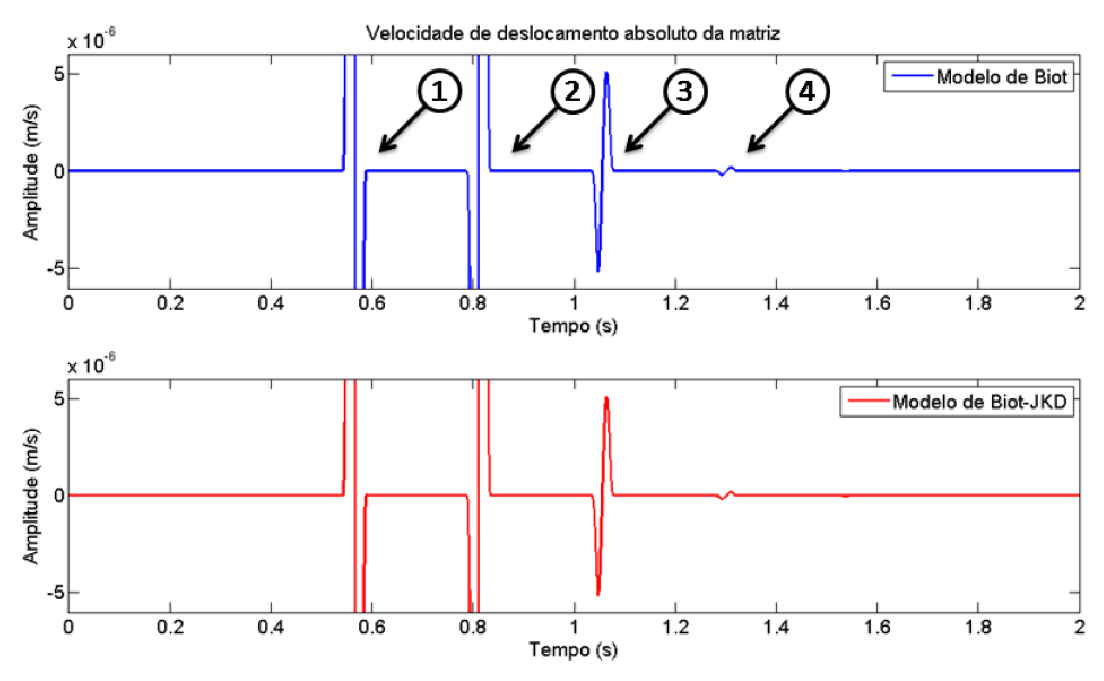
\includegraphics[scale=.65]{igor}
\caption{\textit{Velocidade de deslocamento da matriz para baixas frequ\^encias.}}
\label{fig.igor}
\end{figure}
Al\'em disso, no caso 1D a solu\c{c}\~ao do sistema de Biot pode ser formulada totalmente de maneira anal\'itica e expl\'icita. No caso 3D, todo o c\'odigo computacional s\'o pode ser implementado fazendo uso de opera\c{c}\~oes com matrizes, promovendo desafios em termos de aproxima\c{c}\~oes e instabilidades num\'ericas.


\section{Modelagem Matem\'atica e Num\'erica do Efeito Sismo-Magn\'etico}

Podemos observar uma an\'alise matem\'atica e num\'erica do efeito de indu\c{c}\~ao sismo-magn\'etica em \cite{mikhailenko_97}, onde \'e descrita a solu\c{c}\~ao simult\^anea de equa\c{c}\~oes el\'asticas com o acoplamento da for\c{c}a de Lorentz, e as equa\c{c}\~oes quasi-estacion\'arias de Maxwell com o acoplamento da velocidade de deslocamento do meio de propaga\c{c}\~ao das ondas. Tais sistemas de EDP's foram obtidos do modelo desenvolvido por \cite{Novacki_83} e foram transformados num sistema de EDO's utilizando transformadas finitas de Fourier.

O sistema de EDO's \'e escrito introduzindo uma matriz de vari\'aveis $A$, e a solu\c{c}\~ao num\'erica \'e obtida pelo m\'etodo de fatoriza\c{c}\~ao encontrado em \cite{Mikhailenko_89}, o qual utiliza a matriz de equa\c{c}\~oes de Riccati para a determina\c{c}\~ao das componentes $a_{ij}$. Tal abordagem n\~ao tem restri\c{c}\~oes computacionais se trabalhada com propaga\c{c}\~ao de ondas de alta frequ\^encia.

As simula\c{c}\~oes foram realizadas considerando ondas longitudinais, transversais e Rayleigh. Os resultados  mostraram, principalmente, que as primeiras chegadas das varia\c{c}\~oes geomagn\'eticas coincidiram com as chegadas dos tipos de ondas que as produziram. Essa coincid\^encia ocorreu para onda longitudinal, Rayleigh e para uma onda refletida na interface entre as camadas.

\chapter{Elementos da F\'isica-Matem\'atica}

\section{EDP de uma Onda}
Segundo \cite{farlow_93}, a EDP de uma onda 
\begin{equation}\label{eq.edp_geral}
\frac{\partial^2\mathbf{f}(\mathbf{x},t)}{\partial\,t^2}=\norm{\mathbf{v}}^2\nabla^2\mathbf{f}(\mathbf{x},t)
\end{equation}
possui a solu\c{c}\~ao de D'Alembert
\begin{equation}
\mathbf{f}(\mathbf{x},t)=\mathbf{g}_1(\mathbf{x}-\mathbf{v}\,t)+\mathbf{g}_2(\mathbf{x}+\mathbf{v}\,t),
\end{equation}
onde $\mathbf{x}=(x,y,z)^\top$ representa o espa\c{c}o $\mathbb{R}^3$, $\mathbf{v}$ \'e a \textit{velocidade} de propaga\c{c}\~ao da onda, $(\mathbf{x}\pm\mathbf{v}\,t)$ \'e a \textit{fase} da onda, $\mathbf{g}_1$ \'e a propaga\c{c}\~ao da onda no semiespa\c{c}o positivo do eixo $x$ e $\mathbf{g}_2$ \'e a propaga\c{c}\~ao da onda no semiespa\c{c}o negativo do eixo $x$.

De acordo com \cite{chew}, ondas tridimensionais oriundas de fonte pontual se propagam em formato esferoidal mas localmente podem ser tratadas como ondas planas, principalmente para raios distantes da fonte. A onda esf\'erica, solu\c{c}\~ao da EDP \ref{eq.edp_geral}, pode ser representada pela superposi\c{c}\~ao de ondas planas atrav\'es da identidade de \textit{Weyl}, onde tal superposi\c{c}\~ao tamb\'em \'e solu\c{c}\~ao da EDP \ref{eq.edp_geral}, conforme \cite{weyl_19}.

No $\mathbb{R}^3$ o \textit{vetor de onda} $\mathbf{k}=(k_x,k_y,k_z)^\top$ \'e aquele que aponta na dire\c{c}\~ao de propaga\c{c}\~ao da onda e sua magnitude, denominada \textit{n\'umero de onda}, \'e definida como 
\begin{equation}
\norm{\mathbf{k}}=k=\frac{\omega}{\norm{\mathbf{v}}},
\end{equation}
onde $\omega$ \'e a frequ\^encia temporal. Desta forma, a fase da onda pode ser escrita em termos do vetor de onda e da frequ\^encia como $(\mathbf{k}\cdot\mathbf{x}-\omega\,t)$, e a solu\c{c}\~ao da equa\c{c}\~ao \ref{eq.edp_geral} pode ser reescrita como uma superposi\c{c}\~ao de ondas planas
\begin{equation}
\mathbf{f}(\mathbf{x},t)=\mathbf{A}\,\sum_{\mathbf{k},\omega}{e^{i\,(\mathbf{k}\cdot\mathbf{x}-\omega\,t)}},
\end{equation}
onde $\mathbf{A}$ \'e a \textit{amplitude} da onda.

Podemos verificar em \cite{White_Zhou_2006}, para o caso $\mathbb{R}^2$ o \textit{vetor de onda horizontal} \'e definido como $\mathbf{k}=(k_x,k_y)^\top$, o \textit{n\'umero de onda horizontal} e a \textit{vagarosidade horizontal} s\~ao, respectivamente,
\begin{equation}\label{eq.numero_onda_vagarozidade_horizontal}
k=\sqrt{k_x^2+k_y^2}\qquad\text{e}\qquad\gamma=\frac{k}{\omega}.
\end{equation}
A vagarosidade vertical \'e definida como
\begin{equation}
q_0=\frac{1}{v_z},
\end{equation}
onde $v_z$ \'e a componente vertical da velocidade. Denotando o \textit{n\'umero de onda vertical} por $k_z$, temos que a \textit{vagarosidade vertical} pode ser escrita como
\begin{equation}
q_0=\frac{k_z}{\omega}.
\end{equation}
Combinando as vagarosidades horizontal e vertical, temos
\begin{equation}\label{eq.vagarosidade_vertical}
\gamma^2+q_0^2=\frac{1}{\norm{\mathbf{v}}^2}\qquad\text{ou}\qquad q_0=\sqrt{\epsilon_0\mu_0-\gamma^2},
\end{equation}
j\'a que $\epsilon_0\mu_0=\frac{1}{\norm{\mathbf{v}}^2}$.

\section{Transformadas Laterais de Fourier}

Segundo \cite{butkov_88}, podemos definir as transformadas laterais de Fourier direta e inversa entre o espa\c{c}o bidimensional e o vetor de onda horizontal como
\begin{align}\label{eq.trans_fourier_1}
\mathbf{\widehat{f}}(k_x,k_y,z) &= \iint_{\mathbb{R}^2}\mathbf{f}(x,y,z)\,e^{-i(k_xx+k_yy)}dx\,dy\\\nonumber\\\label{eq.trans_fourier_2}
\mathbf{f}(x,y,z) &= \left(\frac{1}{2\,\pi}\right)^2\iint_{\mathbb{R}^2}\mathbf{\widehat{f}}(k_x,k_y,z)\,e^{i(k_xx+k_yy)}dk_xdk_y.
\end{align}
O s\'imbolo $\,\widehat{}\,$ denota a fun\c{c}\~ao no espa\c{c}o da transformada lateral de Fourier.

A propriedade da transformada de derivadas \'e a que mais nos interessa e, supondo $f$ uma fun\c{c}\~ao escalar de uma \'unica vari\'avel, essa propriedade pode ser descrita como  
\begin{align*}
\widehat{f'}(x)&=\int_{-\infty}^{\infty}f'(x)\,e^{-i\,k_xx}dx\\
&=f(x)\,e^{-i\,k_xx}|_{-\infty}^{\infty}-(-i\,k_x)\int_{-\infty}^{\infty}f(x)\,e^{-i\,k_xx}dx\\
&=i\,k_x\widehat{f}(k_x).
\end{align*}
Na passagem da segunda para a terceira igualdade utilizamos a hip\'otese bastante difundida em geof\'isica de que $f(x)\rightarrow 0$ quando $x \rightarrow \pm \infty $, a qual podemos observar em demonstra\c{c}\~oes de teoremas como, por exemplo, o toerema de \textit{Helmholtz} encontrado em \cite{griffiths}. 


\section{Rota\c{c}\~oes}

Segundo \cite{lang_1986}, podemos produzir uma rota\c{c}\~ao antihor\'aria em torno do eixo $z$ aplicando o operador linear
\begin{equation*}
\begin{pmatrix}
\cos\theta&-\sin\theta&0\\
\sin\theta&\cos\theta&0\\
0&0&1
\end{pmatrix},
\end{equation*}
onde $\theta$ \'e o \^angulo que um vetor est\'a sendo rotacionado. Como a geometria do nosso problema considera ondas se propagando na parte negativa do eixo $z$ (consideramos $z$ positivo no sentido descendente), para produzirmos uma rota\c{c}\~ao antihor\'aria devemos considerar o \^angulo $-\theta$, e com isso nossa matriz de rota\c{c}\~ao se torna
\begin{equation*}
\begin{pmatrix}
\cos\theta&\sin\theta&0\\
-\sin\theta&\cos\theta&0\\
0&0&1
\end{pmatrix},
\end{equation*}
lembrando a paridade das fun\c{c}\~oes seno e cosseno. Para promovermos uma rota\c{c}\~ao orientando a primeira coordenada  no sentido de propaga\c{c}\~ao das ondas horizontais, temos que $\theta$ ser\'a o \^angulo entre $(x,0,0)^\top$ e $(k_x,k_y,0)^\top$, e a matriz de rota\c{c}\~ao se torna
\begin{equation}\label{eq.operador_rotacao}
\Omega=
\begin{pmatrix}
\frac{k_x}{k}&\frac{k_y}{k}&0\\
-\frac{k_y}{k}&\frac{k_x}{k}&0\\
0&0&1
\end{pmatrix}.
\end{equation}
Para escrevermos novamente as equa\c{c}\~oes no sistema de coordenadas original, precisamos aplicar a rota\c{c}\~ao inversa. Para isso, basta inverter a matriz de rota\c{c}\~ao \ref{eq.operador_rotacao} mas, como se trata de uma matriz ortogonal, a inversa \'e a sua transposta. Assim, usaremos
\begin{equation}\label{eq.rotacao_inversa}
\Omega^\top=
\begin{pmatrix}
\frac{k_x}{k}&-\frac{k_y}{k}&0\\
\frac{k_y}{k}&\frac{k_x}{k}&0\\
0&0&1
\end{pmatrix}.
\end{equation}


A rota\c{c}\~ao de um tensor $\tau$ \'e dada por 
\begin{equation}\label{eq.rotacao_tensor}
\tilde{\tau}=\Omega\,\tau\,\Omega^\top,
\end{equation}
e sua rota\c{c}\~ao inversa \'e dada por
\begin{equation}\label{eq.rot_inver_tensor}
\tau=\Omega^\top\tilde{\tau}\,\Omega.
\end{equation}


\section{A fun\c{c}\~ao $\delta$ de Dirac}\label{sec.dirac}

Em algumas aplica\c{c}\~oes f\'isicas pode ser necess\'ario trabalhar com conceito de um pulso de dura\c{c}\~ao infinitamente curta. De acordo com \cite{butkov_88}, podemos tomar o exemplo de um corpo colocado em movimento, a partir do repouso, atrav\'es de um golpe instant\^aneo que faz o mesmo adquirir um momento igual \`a impuls\~ao $I$ do choque, ou seja,
\begin{equation}
I=\int_{t_0}^{t_0+\Delta\,t}f(t)dt,
\end{equation}
onde $f(t)$ \'e a for\c{c}a e $\Delta\,t$ \'e o tempo de a\c{c}\~ao da for\c{c}a. A implus\~ao \'e um n\'umero finito e sua altera\c{c}\~ao ocorre instantaneamente, pois $\Delta\,t$ \'e um n\'umero muito pequeno. Assim, temos que a for\c{c}a deveria ter valor infinito durante o golpe e nula nos outros instantes, conforme o gr\'afico da figura \ref{fig.dirac}.
\begin{figure}
\centering
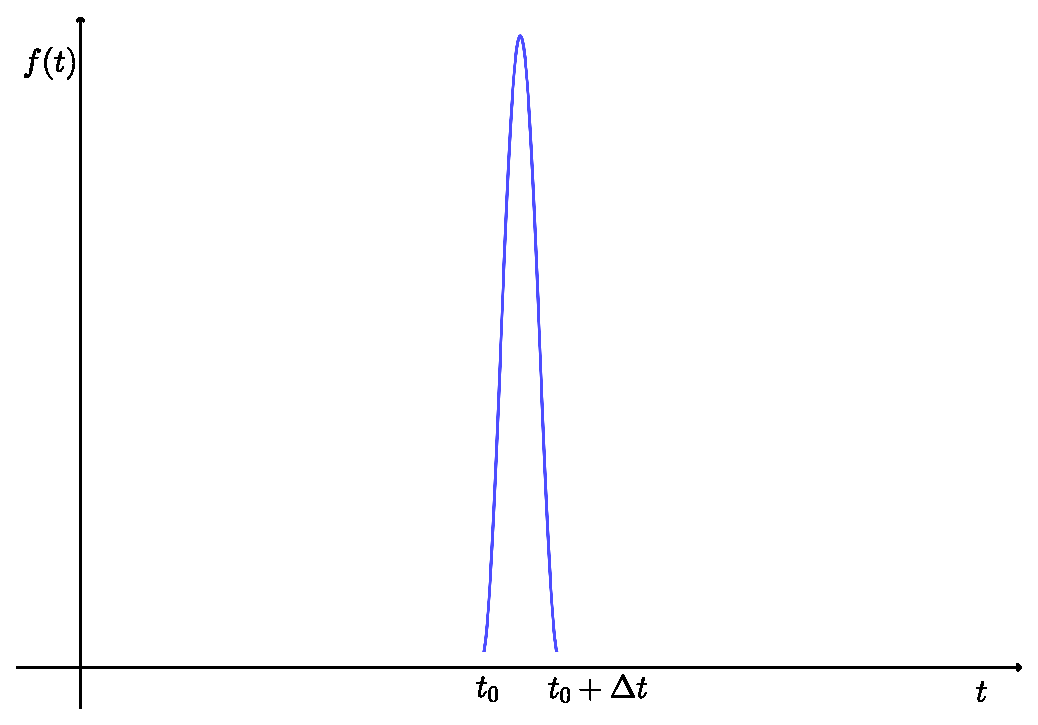
\includegraphics[scale=.6]{dirac_function}
\caption{\textit{Representa\c{c}\~ao de uma fun\c{c}\~ao fortemente concentrada.}}
\label{fig.dirac}
\end{figure}
A fim de facilitar v\'arias opera\c{c}\~oes da f\'isica-matem\'atica, Dirac prop\^os a introdu\c{c}\~ao da chamada fun\c{c}\~ao $\delta(x)$, que pode representar uma fun\c{c}\~ao infinitamente concentrada e \'e dada simbolicamente por
\begin{empheq}[left={\delta(x)=\empheqlbrace}]{align*}
0\,,&\quad\text{se}\quad x\neq 0\\
\infty\,,&\quad\text{se}\quad x=0
\end{empheq}
e $\delta$ deve satisfazer a seguinte condi\c{c}\~ao
\begin{equation}\label{eq.condicao_dirac}
\int_{-\infty}^{\infty}\delta(x)\,dx=1.
\end{equation}
Sendo $f$ uma fun\c{c}\~ao cont\'inua qualquer, a utilidade da fun\c{c}\~ao $\delta$ consiste em determinar o valor de 
\begin{equation}
\int_{-\infty}^{\infty}\delta(x)\,f(x)\,dx
\end{equation}
substituindo os limites de integra\c{c}\~ao por $-\epsilon$ e $\epsilon$, onde $\epsilon$ \'e um n\'umero positivo infinitesimalmente pr\'oximo de zero. Tal substitui\c{c}\~ao se justifica pois $\delta=0$ se $x\neq0$ e teremos uma aproxima\c{c}\~ao para o valor dessa integral. Assim, usando a defini\c{c}\~ao de $\delta$, a condi\c{c}\~ao \ref{eq.condicao_dirac} e a continuidade de $f$, temos
\begin{align*}
\int_{-\infty}^{\infty}\delta(x)\,f(x)\,dx&=\int_{-\infty}^{-\epsilon}\delta(x)\,f(x)\,dx+\int_{-\epsilon}^{\epsilon}\delta(x)\,f(x)\,dx+\int_{\epsilon}^{\infty}\delta(x)\,f(x)\,dx\\
&=\int_{-\epsilon}^{\epsilon}\delta(x)\,f(x)\,dx\\
&\approx\,f(0)\int_{-\epsilon}^{\epsilon}\delta(x)\,dx\\
&=f(0).
\end{align*}
Desta forma podemos representar a aplica\c{c}\~ao de uma fun\c{c}\~ao fortemente concentrada, incluindo a representa\c{c}\~ao de uma fonte pontual de onda s\'ismica que \'e de interesse geof\'isico, como veremos na subse\c{c}\~ao \ref{sec.presenca_fonte}.

\section{Fun\c{c}\~ao de Bessel de Primeira Esp\'ecie}

De acordo com \cite{butkov_88}, sendo $f(x)$ uma fun\c{c}\~ao qualquer, podemos escrever a equa\c{c}\~ao diferencial ordin\'aria de Bessel na forma
\begin{equation}
\frac{d^2f}{dx}+\frac{1}{x}\frac{df}{dx}+\left(1-\frac{m^2}{x^2} \right)\,f=0,
\end{equation}
onde, estudando o caso geral temos que $m$ \'e um n\'umero real arbitr\'ario que pode ser considerado n\~ao-negativo, mas no nosso trabalho vamos considerar $m$ inteiro positivo. A equa\c{c}\~ao acima \'e a EDO de Bessel de ordem $m$, suas solu\c{c}\~oes s\~ao conhecidas como fun\c{c}\~oes cil\'indricas e entre elas est\~ao as fun\c{c}\~oes de Bessel. Expandindo a fun\c{c}\~ao $f(x)$ numa s\'erie de \textit{Frobenius} e substituindo-a  na EDO de Bessel podemos deduzir que a solu\c{c}ao \'e dada por
\begin{equation}\label{eq.funcao_bessel_1}
J_m(x)=\sum_{j=0}^{\infty}(-1)^j\frac{x^{m+2\,j}}{j!\,\Gamma\,(m+j+1)\,2^{m+2\,j}}.
\end{equation}
A fun\c{c}\~ao $\Gamma$ \'e uma fun\c{c}\~ao fatorial de vari\'avel real com representa\c{c}\~ao na forma integral dada por
\begin{equation*}
\Gamma(\xi)=\int_0^\infty t^{\xi-1}e^tdt,\qquad x>0.
\end{equation*}
Como estamos trabalhando com $m$ inteiro positivo, a fun\c{c}\~ao $\Gamma(\xi)$ \'e dada simplesmente por $(\xi-1)!$. Assim, a express\~ao \ref{eq.funcao_bessel_1} passa a ser escrita como
\begin{equation}\label{eq.funcao_bessel_2}
J_m(x)=\sum_{j=0}^{\infty}\frac{(-1)^j}{j!\,(m+j)!}\left(\frac{x}{2}\right)^{m+2\,j}
\end{equation}
e \'e chamada fun\c{c}\~ao de Bessel de primeira esp\'ecie de ordem $m$.

\section{Transformadas de Hankel}\label{sec.trans_hankel}
A transformada de Hankel utiliza as fun\c{c}\~oes de Bessel para transformar um sistema de coordenadas $\mathbf{x}$ para outro $\pmb{\xi}$. De acordo com \cite{baruch_2013}, assumindo que $f$ seja uma fun\c{c}\~ao radial, ou seja, que depende apenas da magnitude $x$ de $\mathbf{x}$, umas das defini\c{c}\~oes da transformada de Hankel \'e dada por
\begin{equation*}
\mathcal{B}_m[f(x)](\xi)=\int_0^\infty x\,J_m(x\,\xi)\,f(x)\,dx.
\end{equation*}
E a transformada inversa, considerando $\xi=\norm{\pmb{\xi}}$, \'e
\begin{equation*}
\mathcal{B}^{-1}_m[F(\xi)](x)=\int_0^\infty \xi\,J_m(x\,\xi)\,F(\xi)\,d\xi,
\end{equation*}
onde $J_m$ \'e uma fun\c{c}\~ao de Bessel de primeira esp\'ecie de ordem $m$, conforme visto na subse\c{c}\~ao anterior.











\chapter{M\'etodo Matricial para Solu\c{c}\~ao de EDO's}

Este cap\'itulo trata do estudo do m\'etodo matricial para analisar a propaga\c{c}\~ao de ondas em subsuperf\'icie terrestre, conforme estruturado em \cite{Ursin-1983}. Gra\c{c}as a similaridade matem\'atica entre sistemas de EDP's eletromagn\'eticas (Maxwell) e sistemas de EDP's el\'asticas (Lamè), podemos dar um desenvolvimento unificado para esses sistemas. Utilizamos um conjunto de transformadas e mudan\c{c}a de eixos coordenados para dividir esses dois sistemas de EDP's em quatro sistemas de EDO's escritos em forma matricial, onde as vari\'aveis dependentes estejam em fun\c{c}\~ao apenas da profundidade e da frequ\^encia temporal. Os coeficientes desses sistemas de EDO's podem ser reunidos numa matriz $M$ de dimens\~ao $2n\times 2n$, a qual pode ser particionada em quatro submatrizes de dimens\~ao $n\times n$, e \'e usada como o ponto de partida para o estudo da propaga\c{c}\~ao de ondas em subsuperf\'icie.  

As propriedades de simetria da matriz $M$ nos permitem separar o campo de ondas em ascendentes e descendentes atrav\'es de uma decomposi\c{c}\~ao em autovetores. Essas propriedades nos permitem tamb\'em deduzir caracter\'isticas invariantes da propaga\c{c}\~ao, onde uma dessas caracter\'isticas \'e v\'alida apenas para meios de baixa dissipa\c{c}\~ao de ondas e correspondem \`a conserva\c{c}\~ao de energia. A matriz de propaga\c{c}\~ao de ondas pode ser computada para camadas homog\^eneas ou n\~ao, atrav\'es de um m\'etodo relativamente simples. Dado o vetor de ondas na camada superficial, podemos calcular seu valor para qualquer camada usando a matriz de propaga\c{c}\~ao.

A propaga\c{c}\~ao de ondas em meios estratificados produz fen\^omenos de transmiss\~ao e reflex\~ao de ondas. Dadas as dedu\c{c}\~oes das matrizes de transmiss\~ao e reflex\~ao, podemos relacion\'a-las com a matriz de propaga\c{c}\~ao, bem como deduzir propriedades de simetrias para essas matrizes atrav\'es das caracter\'isticas invariantes da propaga\c{c}\~ao. Podemos ainda deduzir as matrizes de transmiss\~ao e reflex\~ao modificadas para pilha de camadas limitadas superiormente por uma superf\'icie livre.

\section{Caracter\'isticas das Equa\c{c}\~oes na Forma Matricial de Ursin}

%Sendo $\mathbf{x}=(x,y,z)^{\top}$ o espa\c{c}o $\mathbb{R}^3$ e aplicando as tranformadas de Fourier direta e inversa na forma
%\begin{align*}
%F(\omega,k_1,k_2,z) &= \iiint_{-\infty}^{\infty}f(t,x,y,z)\,e^{i\omega t-ik_1x-ik_2y}dt\,dxdy\\\\
%f(t,x,y,z) &= \left(\frac{1}{2\,\pi}\right)^3\,\iiint_{-\infty}^{\infty}F(\omega,k_1,k_2,z)\,e^{-i\omega t+ik_1x+ik_2y}d\omega\,dk_1dk_2\,,
%\end{align*}
%podemos escrever um conjunto de EDP's que descevem a propaga\c{c}\~ao de ondas sismomagn\'eticas em camadas horizontais da subsuperf\'icie terrestre somente em fun\c{c}\~ao da profundidade $z$. 
%
%A t\'itulo de exemplo, tanto as EDP's de Maxwell para o eletromagnetismo
%\begin{align}\label{eq.faraday_ampere}\nonumber
%\nabla\times\mathbf{E}&=-\frac{\partial}{\partial t}\mathbf{B}\\\\\nonumber
%\nabla\times\mathbf{H}&=\sigma\mathbf{E}+\frac{\partial}{\partial t}\mathbf{D}+\mathbf{G}\,,
%\end{align}
%como as EDP's el\'asticas
%\begin{align}\label{eq.cauchy_hooke}\nonumber
%\rho\frac{\partial^2 \mathbf{U}}{\partial t^2}&=\nabla\cdot\tau+\mathbf{F}\\\\\nonumber
%\tau&=\lambda\nabla\cdot \mathbf{U}\cdot I + \mu(\nabla \mathbf{U}+\nabla \mathbf{U}^*)\,,
%\end{align}
%podem ser escritas no formato matricial apresentado por Ursin, ou seja, 
\'E poss\'ivel utilizar o m\'etodo matricial no formato preconizado por \cite{Ursin-1983} para resolver sistemas de EDO's desde que se possa escrever tal sistema como
\begin{align}\label{eq.matricial}
\frac{\partial\,\mathbf{\Phi}^{(m)}}{\partial\,z} &= -\,i\,\omega\,M^{(m)}\,\mathbf{\Phi}^{(m)}+\mathbf{S}^{(m)},\quad\text{com}\quad m\,\in\mathbb{N},
\end{align}
%\begin{bmatrix}
%\mathbf{\Phi_1}\\
%\mathbf{\Phi_2}	
%\end{bmatrix}\,,
onde $\mathbf{S}^{(m)}$ \'e um vetor de fonte de onda s\'ismica de dimens\~ao $2\,n_m$ e as matrizes $M^{(m)}_{2\,n_m\times2\,n_m}$ t\^em o formato
\begin{equation}\label{eq.matriz_M}
M^{(m)}
=
\begin{pmatrix}
\mathbf{0}&M_1^{(m)}\\
M_2^{(m)}&\mathbf{0}
\end{pmatrix},
\end{equation}
onde $M_1^{(m)}$ e $M_2^{(m)}$ s\~ao submatrizes sim\'etricas de dimens\~ao $n_m\times n_m$.

A equa\c{c}\~ao \ref{eq.matricial} tem as seguintes caracter\'isticas:
\begin{itemize}
\item $M^{(m)}_{2\,n\times2\,n}$ \'e uma matriz que pode ser particionada em quatro submatrizes $n\times n$, com submatrizes de zeros na diagonal principal e submatrizes sim\'etricas $M_1^{(m)}$ e $M_2^{(m)}$ na diagonal secund\'aria. As componentes de $M_1^{(m)}$ e $M_2^{(m)}$ s\~ao fun\c{c}\~oes dos par\^ametros das EDP's que est\~ao sendo trabalhadas, s\~ao fun\c{c}\~oes tamb\'em de $z$ e do vetor real de vagarosidade $\pmb{\gamma}=\frac{\mathbf{k}}{\omega}$. Para meios de baixa dissipa\c{c}\~ao das ondas, as matrizes $M_1^{(m)}$ e $M_2^{(m)}$ s\~ao reais; 
\item O vetor de onda $\mathbf{\Phi}^{(m)}$ tem dimens\~ao $2n\times1$ e \'e particionado em dois vetores $\mathbf{\Phi}^{(m)}_1$ e $\mathbf{\Phi}^{(m)}_2$ com dimens\~ao $n\times1$ . As componentes do vetor de onda s\~ao escolhidas de forma que $\mathbf{\Phi}^{(m)}$ seja cont\'inuo atrav\'es das fronteiras entre duas camadas;
\item  Para ondas el\'asticas, metade das componentes de $\mathbf{\Phi}^{(m)}$ s\~ao zeros na superf\'icie livre, ou seja, existe uma matriz de permuta\c{c}\~ao $T_{2n\times2n}$ onde $T^{-1}=T^\top$ e tal que
\begin{equation*}
\begin{bmatrix}
\mathbf{V}_1(\mathbf{0})\\
\mathbf{0}
\end{bmatrix}
=T\,\mathbf{\Phi}^{(m)}\quad\text{quando}\quad z = 0\,;
\end{equation*}
\item As componentes do vetor de onda $\mathbf{\Phi}^{(m)}$ s\~ao escolhidas de forma que o fluxo de energia na dire\c{c}\~ao $z$ seja dado por
\begin{equation*}
J=-\frac{1}{4}(\mathbf{\Phi}_1^{(m)\,H}\mathbf{\Phi}^{(m)}_2+\mathbf{\Phi}_2^{(m)\,H}\mathbf{\Phi}^{(m)}_1)=-\frac{1}{4}\mathbf{\Phi}^{(m)\,H}\,M_0\mathbf{\Phi}^{(m)}\,,
\end{equation*}
onde $H$ denota complexo conjugado transposto,
\begin{equation*}
M_0=
\begin{bmatrix}
0_{n\times n}&I\\
I&0_{n\times n}
\end{bmatrix}
\end{equation*}
e $I$ \'e uma matriz identidade $n\times n$.
\end{itemize}

O m\'etodo a seguir \'e aplicado em equa\c{c}\~oes escritas no formato matricial \ref{eq.matricial}, com ondas se propagando numa pilha de camadas homog\^eneas e assumimos que os par\^ametros das equa\c{c}\~oes s\~ao fun\c{c}\~oes cont\'inuas no interior de cada camada e que dependem apenas da profundidade $z$. O modelo inclui pilha de camadas homog\^eneas com par\^ametros constantes por camada e consideramos o eixo $z$ como sendo positivo no sentido descendente.

\section{Diagonaliza\c{c}\~ao}\label{sec.diagonalizacao}
Considere matrizes $M$ conforme a equa\c{c}\~ao \ref{eq.matriz_M}, onde por simplicidade de escrita n\~ao usaremos o sobrescrito $m$. Vamos aplicar nesta matriz um procedimento de diagonaliza\c{c}\~ao que pode ser encontrado em trabalhos como \cite{Ursin-1983}, \cite{White_Zhou_2006} e \cite{Azeredo_2013}.

Seja $(\mathbf{a}_m,\,\mathbf{b}_m)^\top$ seja um autovetor da matriz $M$ associado ao autovalor $q_m$, com $m=1,...,n$, assim
\begin{equation}
\begin{pmatrix}
0_{n\times n}&M_1\\
M_2&0_{n\times n}
\end{pmatrix}
\begin{pmatrix}
\mathbf{a}_m\\
\mathbf{b}_m
\end{pmatrix}
=
q_m\,
\begin{pmatrix}
\mathbf{a}_m\\
\mathbf{b}_m
\end{pmatrix}.
\end{equation}
Ou seja, 
\begin{equation}\label{eq.M1_b}
M_1\mathbf{b}_m=q_m\,\mathbf{a}_m 
\end{equation}
e
\begin{equation}\label{eq.M2_a}
M_2\mathbf{a}_m=q_m\,\mathbf{b}_m. 
\end{equation}
Multiplicando \ref{eq.M1_b} pela esquerda por $M_2$ e substituindo \ref{eq.M2_a}, temos
\begin{equation}\label{eq.m2m1bm}
M_2M_1\mathbf{b}_m=q_m^2\mathbf{b}_m.
\end{equation} 
Analogamente, multiplicando \ref{eq.M2_a} pela esquerda por $M_1$ substituindo \ref{eq.M1_b}, temos 
\begin{equation}\label{eq.m1m2am}
M_1M_2\mathbf{a}_m=q_m^2\mathbf{a}_m.
\end{equation}
Desta forma, $\mathbf{a}_m$ \'e um autovetor associado \`a matriz $M_1M_2$, e $\mathbf{b}_m$ \'e um autovetor associado \`a matriz $M_2M_1$. 

Como estamos assumindo que $M_1$ e $M_2$ s\~ao sim\'etricas, partindo da equa\c{c}\~ao \ref{eq.m2m1bm} e usando a equa\c{c}\~ao \ref{eq.m1m2am}, temos
\begin{align*}
q_m^2\mathbf{b}_m&=M_2M_1\mathbf{b}_m\\
q_m^2\mathbf{a}_j^\top\mathbf{b}_m&=\mathbf{a}_j^\top M_2M_1\mathbf{b}_m\\
&=\mathbf{b}_m^\top M_1M_2\mathbf{a}_j\\
&=q_j^2\mathbf{a}_j^\top\mathbf{b}_m.
\end{align*}
Isolando $\mathbf{a}_j^\top\mathbf{b}_m$ na \'ultima igualdade acima, temos que 
\begin{empheq}[left={\mathbf{a}_j^\top\mathbf{b}_m=\empheqlbrace}]{align}\label{eq.ajTbm}\nonumber
0\,,&\quad\text{se}\quad m\neq j\\\\\nonumber
\alpha_{j,m}\,,&\quad\text{se}\quad m=j,
\end{empheq}
onde $\alpha$ \'e um valor indeterminado.

Vamos definir a matriz $L_1$ de dimens\~ao $n\times n$ onde cuja $m$-\'esima coluna \'e dada por $\mathbf{a}_m$, e a matriz $L_2$ tamb\'em de dimens\~ao $n\times n$ cuja $m$-\'esima coluna \'e dada por $\mathbf{b}_m$. Assim, podemos reescrever as equa\c{c}\~oes \ref{eq.M1_b} e \ref{eq.M2_a}, respectivamente, como
\begin{align}\label{eq.m1l2}
M_1L_2&=L_1\Lambda\\\label{eq.m2l1}
M_2L_1&=L_2\Lambda,
\end{align}
onde a matriz $\Lambda_{n\times n}$ \'e a matriz diagonal dos autovalores. Observe que podemos trabalhar com as equa\c{c}\~oes normalizadas tomando $\alpha_{j,m}=1$ na equa\c{c}\~ao \ref{eq.ajTbm}, que passa a definir o s\'imbolo \textit{Delta de Kroneker}\footnote{Nos abstivemos de usar o caracter grego $\delta$ na equa\c{c}\~ao \ref{eq.ajTbm} por este j\'a definir a fun\c{c}\~ao Delta de Dirac em nosso escopo.}, conforme \cite{lebedev_2003}. Assim, escrevemos as componentes de $\Lambda$ como $\Lambda_{j,m}=q_j\mathbf{a}_j^\top\mathbf{b}_m$. Observe ainda que, deste modo, a equa\c{c}\~ao \ref{eq.ajTbm} define a matriz identidade $I_{n\times n}$, a qual podemos usar para mostrar que
\begin{align}\label{eq.l1l2}
L_1^{-1}&=L_2^\top\\\label{eq.l2l1}
L_2^{-1}&=L_1^\top.
\end{align}
Multiplicando pela direita as equa\c{c}\~oes \ref{eq.m1l2} e \ref{eq.m2l1} respectivamente por $L_2^{-1}$ e $L_1^{-1}$, e substituindo as equa\c{c}\~oes \ref{eq.l1l2} e \ref{eq.l2l1}, temos
\begin{align}
M_1&=L_1\Lambda L_1^\top\\
M_2&=L_2\Lambda L_2^\top.
\end{align}
Definindo a matriz $L_{2\,n\times 2\,n}$ como
\begin{equation}\label{eq.matriz_L}
L=\frac{1}{\sqrt{2}}
\begin{pmatrix}
L_1&L_1\\
L_2&-L_2
\end{pmatrix},
\end{equation}
e a matriz $\tilde{\Lambda}$ como
\begin{equation}\label{eq.tildeLambda}
\tilde{\Lambda}=
\begin{pmatrix}
\Lambda&0\\
0&-\Lambda
\end{pmatrix},
\end{equation}
podemos deduzir que
\begin{equation}\label{eq.L^-1}
L^{-1}=\frac{1}{\sqrt{2}}
\begin{pmatrix}
L_2^\top&L_1^\top\\
L_2^\top&-L_1^\top
\end{pmatrix}
\end{equation}
e
\begin{equation}\label{eq.m_semelhante_lambda}
M=L\,\tilde{\Lambda}\,L^{-1}.
\end{equation}

\section{Solu\c{c}\~ao de EDO's na Aus\^encia de Fonte}\label{sec.ausencia_fonte}

Vamos determinar inicialmente a solu\c{c}\~ao de EDO's  considerando o meio homog\^eneo e livre de fonte de onda s\'ismica. Ap\'os a diagonaliza\c{c}\~ao dessas equa\c{c}\~oes, podemos aplicar um m\'etodo utilizado por alguns autores como \cite{Ursin-1983}, \cite{Azeredo_2013}, \cite{White_Zhou_2006}, \cite{miranda_2016} entre outros, para determinar as solu\c{c}\~oes na aus\^encia de fonte. Esse mesmo m\'etodo pode ser utilizado para determinar as solu\c{c}\~oes na presen\c{c}a de fonte como veremos no cap\'itulo \ref{sec.presenca_fonte}. Aus\^encia de fonte significa que temos $\mathbf{S}^{(m)}=0$ na equa\c{c}\~ao \ref{eq.matricial}. A matriz ${M}^{(m)}$ possui entradas constantes por camada estratigr\'afica, as submatrizes na diagonal principal s\~ao nulas e as submatrizes na diagonal secund\'aria s\~ao sim\'etricas. 

\subsection{Ondas Ascendentes e Ondas Descendentes}

Vamos redefinir o vetor de ondas como
\begin{equation}\label{eq.Phi}
\mathbf{\Phi}=L\,\mathbf{\Psi}.
\end{equation}
Substituindo a equa\c{c}\~ao \ref{eq.Phi} na equa\c{c}\~ao \ref{eq.matricial}, temos
\begin{equation}\label{eq.matricial_sem_fonte}
\frac{\partial\,\mathbf{\Psi}}{\partial\,z} =-\,i\,\omega\,L^{-1}M\,L\,\mathbf{\Psi},
\end{equation}
onde o sobrescrito $m$ est\'a sendo omitido por quest\~ao de simplicidade.
De acordo com a equa\c{c}\~ao \ref{eq.m_semelhante_lambda}, temos que as matrizes $M$ e $\tilde{\Lambda}$ s\~ao semelhantes, assim
\begin{equation*}
\tilde{\Lambda}=L^{-1}M\,L.
\end{equation*}
Substituindo $\tilde{\Lambda}$ na equa\c{c}\~ao \ref{eq.matricial_sem_fonte}, temos
\begin{equation}\label{eq.matricial_sem_fonte_2}
\frac{\partial\,\mathbf{\Psi}}{\partial\,z} =-\,i\,\omega\,\tilde{\Lambda}\,\mathbf{\Psi}.
\end{equation}
De acordo com a equa\c{c}\~ao \ref{eq.tildeLambda}, $\tilde{\Lambda}$ \'e uma matriz cuja diagonal principal cont\'em a submatriz $\Lambda$, onde $\Lambda$ \'e uma matriz diagonal contendo os autovalores $q_i$.
Definindo
\begin{equation}\label{eq.definicao_psi}
\mathbf{\Psi}=
\begin{pmatrix}
\mathbf{U}\\
\mathbf{D}
\end{pmatrix}
\end{equation}
e usando o fato de que $\tilde{\Lambda}$ \'e uma matriz diagonal, podemos resolver a equa\c{c}\~ao diferencial \ref{eq.matricial_sem_fonte_2} e expressar a solu\c{c}\~ao na forma
\begin{align}\nonumber
\mathbf{\Psi}(z)&=e^{-i\,\omega\,\tilde{\Lambda}(z-z_0)}\mathbf{\Psi}(z_0)\\\label{eq.solucao_psi}
&=\begin{pmatrix}
e^{-i\,\omega\,\Lambda(z-z_0)}\,\mathbf{U}(z_0)\\
e^{i\,\omega\,\Lambda(z-z_0)}\,\,\,\mathbf{D}(z_0)
\end{pmatrix}.
\end{align}
Desta maneira, $\mathbf{U}$ representa ondas ascendentes e $\mathbf{D}$ representa ondas descendentes, $z_0$ \'e um ponto fixo na mesma regi\~ao livre de fonte de $z$ e $e^{\pm i\,\omega\,\Lambda(z-z_0)}$ \'e uma matriz diagonal onde o $j$-ésimo elemento da diagonal principal \'e dado por $e^{\pm i\,\omega\,q_j(z-z_0)}$. 

\subsection{Matriz de Salto para Camadas Estratificadas}

A profundidade onde encontra-se uma interface entre duas camadas estratificadas ser\'a denotada por $\overline{z}$, onde as quantidades avaliadas imediatamente abaixo da interface ser\'a denotada por $\overline{z}^+$ e as quantidades avaliadas imediatamente acima da interface ser\'a denotada por $\overline{z}^-$.
De acordo com \cite{White_Zhou_2006}, temos a continuidade de $\mathbf{\Phi}$ atrav\'es das fronteiras entre as camadas, assim \'e v\'alida a rela\c{c}\~ao $\mathbf{\Phi}^+=\mathbf{\Phi}^-$. Substituindo a equa\c{c}\~ao \ref{eq.Phi}, temos 
\begin{align}\nonumber
L^+\mathbf{\Psi}^+&=L^-\mathbf{\Psi}^-\\\nonumber
\mathbf{\Psi}^+&=(L^+)^{-1}L^-\mathbf{\Psi}^-\\\label{eq.psi_matriz_salto}
\mathbf{\Psi}^+&=J\,\mathbf{\Psi}^-,
\end{align}
onde $J=(L^+)^{-1}L^-$ \'e denominada \textit{matriz de salto}. Substituindo a equa\c{c}\~ao \ref{eq.matriz_L}, podemos expressar a matriz de salto como
\begin{equation}
J=
\begin{pmatrix}
J_A&J_B\\
J_B&J_A
\end{pmatrix},
\end{equation}
onde $J_A$ e $J_B$ s\~ao dadas por
\begin{align}\label{eq.j_a}
J_A&=\frac{1}{2}\left[(L_2^+)^\top L_1^-+(L_1^+)^\top L_2^-\right]\\\label{eq.j_b}
J_B&=\frac{1}{2}\left[(L_2^+)^\top L_1^--(L_1^+)^\top L_2^-\right].
\end{align}
Com outra simples multiplica\c{c}\~ao de matrizes temos que
\begin{align}\nonumber
J^{-1}&=(L^-)^{-1}L^+\\\label{eq.inversa_matriz_salto}
&=
\begin{pmatrix}
J_A^\top&-J_B^\top\\
-J_B^\top&J_A^\top
\end{pmatrix}.
\end{align}

\subsection{Matriz de Reflex\~ao e Matriz de Transmiss\~ao}

Considere um meio estratificado, homog\^eneo no interior de cada camada, com $N$ interfaces nas profundidades $0<z_1<z_2<...<z_N<\infty$ e sem exist\^encia de fonte nessas camadas. 

\subsubsection{Reflex\~ao e Transmiss\~ao na \'Ultima Interface}
Pela figura \ref{fig.ondas_em_zn}, considerando que n\~ao h\'a ondas ascendentes depois da \'ultima interface em $z=z_N$, podemos substituir a defini\c{c}\~ao \ref{eq.definicao_psi} na equa\c{c}\~ao \ref{eq.psi_matriz_salto} e obter
\begin{align*}
\mathbf{\Psi}_N^-&=J_N^{-1}\,\mathbf{\Psi}_N^+\\\\
\begin{pmatrix}
\mathbf{U}_N^-\\
\mathbf{D}_N^-
\end{pmatrix}
&=J_N^{-1}\,
\begin{pmatrix}
0\\
\mathbf{D}_N^+
\end{pmatrix}.
\end{align*}

\begin{figure}
\centering
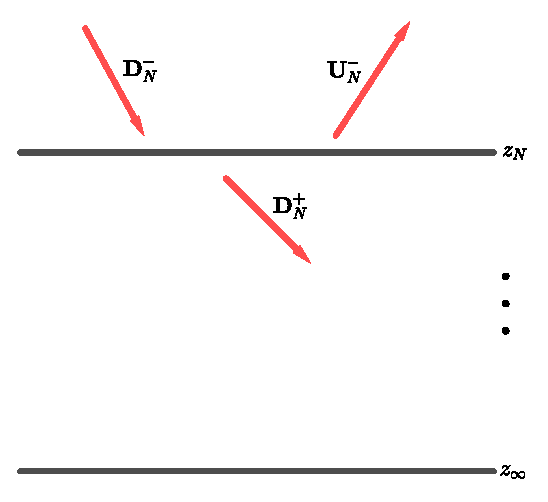
\includegraphics[scale=1]{ondas_em_zn}
\caption{\textit{Ondas ascendentes e descendentes na \'ultima interface. Observe que n\~ao h\'a ondas ascendentes depois da \'ultima camada}.}
\label{fig.ondas_em_zn}
\end{figure}

Substituindo a equa\c{c}\~ao \ref{eq.inversa_matriz_salto} na equa\c{c}\~ao anterior, temos
\begin{align*}
\begin{pmatrix}
\mathbf{U}_N^-\\
\mathbf{D}_N^-
\end{pmatrix}
&=
\begin{pmatrix}
J_{A,N}^\top&-J_{B,N}^\top\\
-J_{B,N}^\top&J_{A,N}^\top
\end{pmatrix}
\,
\begin{pmatrix}
0\\
\mathbf{D}_N^+
\end{pmatrix}\\\\
&=
\begin{pmatrix}
-J_{B,N}^\top \mathbf{D}_N^+\\
 J_{A,N}^\top \mathbf{D}_N^+
\end{pmatrix},
\end{align*}
ou seja,
\begin{align*}
\mathbf{U}_N^-&=-J_{B,N}^\top J_{A,N}^{-\top}\mathbf{D}_N^-\\
\mathbf{D}_N^+&=J_{A,N}^{-\top}\mathbf{D}_N^-.
\end{align*}
Assim, vemos que para computar uma onda refletida, ou seja, uma onda ascendente a partir de uma interface entre camadas, usamos uma \textit{matriz de reflex\~ao} que fica definida como
\begin{equation}\label{eq.reflexao_N}
\Gamma_N=-J_{B,N}^\top J_{A,N}^{-\top}.
\end{equation} 
Analogamente, vemos que para computar uma onda transmitida, ou seja, uma onda descendente a partir de uma interface entre camadas, usamos uma \textit{matriz de transmiss\~ao} que fica definida como
\begin{equation}\label{eq.transmissao_N}
T_N=J_{A,N}^{-\top}.
\end{equation} 

\subsubsection{Reflex\~ao e Transmiss\~ao numa Interface Qualquer}
Definimos a espessura de uma camada, a partir da interface superior, como
\begin{equation}
\Delta\,z_m=z_{m+1}-z_m,\qquad m=1,2,...,N-1,
\end{equation}
e temos que uma onda se propagando da interface na profundidade $z_m$ at\'e a interface em $z_{m+1}$ percorre uma profundidade total $\Delta\,z_m$. O valor dessa onda no fim da trajet\'oria, quando $z=z_{m+1}$, \'e aproximadamente igual a $\mathbf{\Psi}^-_{m+1}$, conforme a figura \ref{fig.N_interfaces}. Assim, usando a solu\c{c}\~ao \ref{eq.solucao_psi} podemos escrever
\begin{equation}\label{eq.solucao_delta_zm}
\mathbf{\Psi}^-_{m+1}=e^{-i\,\omega\tilde{\Lambda}_m\Delta\,z_m}\mathbf{\Psi}^+_m.
\end{equation}

\begin{figure}
\centering
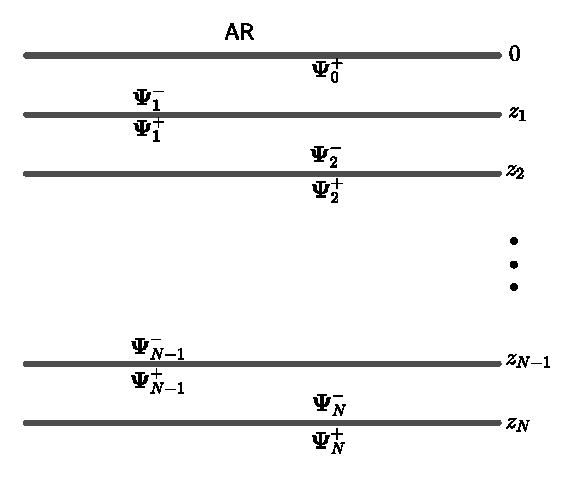
\includegraphics[scale=1]{n_interfaces}
\caption{\textit{Visualiza\c{c}\~ao de $N$ interfaces em subsuperf\'icie e a nota\c{c}\~ao das ondas nas proximadades de cada interface.}}
\label{fig.N_interfaces}
\end{figure}

Sabendo que essa onda se propagando na camada abaixo da interface em $z_m$ veio da camada anterior, podemos usar a matriz de salto na equa\c{c}\~ao \ref{eq.psi_matriz_salto} e escrever
\begin{align}\label{eq.salto_m}
\mathbf{\Psi}^+_{m}&=J_m\,\mathbf{\Psi}^-_m.
\end{align}
Substituindo a equa\c{c}\~ao \ref{eq.salto_m} na equa\c{c}\~ao \ref{eq.solucao_delta_zm}, temos
\begin{align}\label{eq.psi_m-}\nonumber
\mathbf{\Psi}^-_{m+1}&=e^{-i\,\omega\tilde{\Lambda}_m\Delta\,z_m}\mathbf{\Psi}^+_m\\\nonumber
\mathbf{\Psi}^-_{m+1}&=e^{-i\,\omega\tilde{\Lambda}_m\Delta\,z_m}J_m\,\mathbf{\Psi}^-_m\\
\mathbf{\Psi}^-_m&=J^{-1}_me^{i\,\omega\tilde{\Lambda}_m\Delta\,z_m}\mathbf{\Psi}^-_{m+1}
\end{align}
Substituindo a equa\c{c}\~ao \ref{eq.definicao_psi} e a equa\c{c}\~ao \ref{eq.inversa_matriz_salto} na equa\c{c}\~ao \ref{eq.psi_m-}, temos
\begin{align}\label{eq.refle_trans_1}
\mathbf{U}_m^-&=J^\top_{A,m}e^{i\,\omega\Lambda_m\Delta\,z_m}\mathbf{U}^-_{m+1}-J^\top_{B,m}e^{-i\,\omega\Lambda_m\Delta\,z_m}\mathbf{D}^-_{m+1}\\\nonumber\\\label{eq.refle_trans_2}
\mathbf{D}_m^-&=-J^\top_{B,m}e^{i\,\omega\Lambda_m\Delta\,z_m}\mathbf{U}^-_{m+1}+J^\top_{A,m}e^{-i\,\omega\Lambda_m\Delta\,z_m}\mathbf{D}^-_{m+1}.
\end{align}
Assim como definimos matriz de reflex\~ao para a \'ultima interface em $z_N$, podemos definir a matriz de reflex\~ao para uma interface qualquer, ou seja,
\begin{equation}\label{eq.reflexao_m+1}
\mathbf{U}^-_{m+1}=\Gamma_{m+1}\mathbf{D}^-_{m+1}.
\end{equation}
Substituindo a equa\c{c}\~ao \ref{eq.reflexao_m+1} na equa\c{c}\~ao \ref{eq.refle_trans_1} e na equa\c{c}\~ao \ref{eq.refle_trans_2}, temos
\begin{align}\label{eq.refle_trans_3}
\mathbf{U}_m^-&=(J^\top_{A,m}e^{i\,\omega\Lambda_m\Delta\,z_m}\Gamma_{m+1}-J^\top_{B,m}e^{-i\,\omega\Lambda_m\Delta\,z_m})\mathbf{D}^-_{m+1}\\\nonumber\\\label{eq.refle_trans_4}
\mathbf{D}_m^-&=(-J^\top_{B,m}e^{i\,\omega\Lambda_m\Delta\,z_m}\Gamma_{m+1}+J^\top_{A,m}e^{-i\,\omega\Lambda_m\Delta\,z_m})\mathbf{D}^-_{m+1}\,.
\end{align}
Substituindo a equa\c{c}\~ao \ref{eq.refle_trans_4} na equa\c{c}\~ao \ref{eq.refle_trans_3}, temos
\begin{align*}
\mathbf{U}_m^-&=(J^\top_{A,m}e^{i\,\omega\Lambda_m\Delta\,z_m}\Gamma_{m+1}-J^\top_{B,m}e^{-i\,\omega\Lambda_m\Delta\,z_m})\\
&\,\,\cdot\,\,(-J^\top_{B,m}e^{i\,\omega\Lambda_m\Delta\,z_m}\Gamma_{m+1}+J^\top_{A,m}e^{-i\,\omega\Lambda_m\Delta\,z_m})^{-1}\mathbf{D}_m^-\,,
\end{align*}
de onde podemos concluir que a matriz de reflex\~ao em uma interface em $z_m$ qualquer \'e dada por
\begin{align*}
\Gamma_{m}&=(J^\top_{A,m}e^{i\,\omega\Lambda_m\Delta\,z_m}\Gamma_{m+1}-J^\top_{B,m}e^{-i\,\omega\Lambda_m\Delta\,z_m})\\
&\,\,\cdot\,\,(-J^\top_{B,m}e^{i\,\omega\Lambda_m\Delta\,z_m}\Gamma_{m+1}+J^\top_{A,m}e^{-i\,\omega\Lambda_m\Delta\,z_m})^{-1},
\end{align*}
ou
\begin{align}\nonumber
\Gamma_{m}&=(J^\top_{A,m}e^{i\,\omega\Lambda_m\Delta\,z_m}\Gamma_{m+1}e^{i\,\omega\Lambda_m\Delta\,z_m}-J^\top_{B,m})\\\label{eq.matriz_reflexao_m}
&\,\,\cdot\,\,(-J^\top_{B,m}e^{i\,\omega\Lambda_m\Delta\,z_m}\Gamma_{m+1}e^{i\,\omega\Lambda_m\Delta\,z_m}+J^\top_{A,m})^{-1}.
\end{align}
Quando uma onda atinge uma interface, al\'em da possibilidade de reflex\~ao h\'a tamb\'em a possibilidade de trasmiss\~ao da onda para a camada inferior. De maneira an\'aloga ao desenvolvido para reflex\~ao de ondas, podemos deduzir a matriz para a transmiss\~ao de ondas em uma interface qualquer, que \'e dada por
\begin{equation}\label{eq.matriz_transmissao_m}
T_m=T_{m+1}e^{i\,\omega\,\Lambda\Delta\,z_m}(-J^\top_{B,m}e^{i\,\omega\Lambda_m\Delta\,z_m}\Gamma_{m+1}e^{i\,\omega\Lambda_m\Delta\,z_m}+J^\top_{A,m})^{-1}.
\end{equation}
A validade das equa\c{c}\~oes \ref{eq.matriz_reflexao_m} e \ref{eq.matriz_transmissao_m} para qualquer interface pode ser demonstrada por indu\c{c}\~ao sobre $m$, e todas as matrizes de reflex\~ao e transmiss\~ao podem ser computadas por recurss\~ao partindo das equa\c{c}\~oes \ref{eq.reflexao_N} e \ref{eq.transmissao_N}.

\section{Solu\c{c}\~ao na Presen\c{c}a de Fonte}\label{sec.presenca_fonte}
Em prospec\c{c}\~ao de petr\'oleo s\~ao utilizadas alguns tipos de fontes de ondas, atrav\'es das quais se faz um mapeamento das caracter\'isticas das camadas de subsuperf\'icie. Segundo \cite{dobrin_88}, esses tipos de fontes podem ser uma queda de peso, um caminh\~ao \textit{vibroseis}, explosivos e canh\~ao de ar, esta \'ultima fonte utilizada em prospec\c{c}\~ao mar\'itima. Sendo assim, vamos desenvolver uma solu\c{c}\~ao para o nosso problema considerando agora a presen\c{c}a de uma fonte.

Considere ainda a equa\c{c}\~ao \ref{eq.matricial} com o sobrescrito $m$ omitido. Uma fonte $\mathbf{S}$ localizada numa profundidade $z_s$ pode ser representada na forma
\begin{equation}\label{eq.fonte_geral}
\mathbf{S}=\mathbf{S}_0\delta(z-z_s)+\mathbf{S}_1\delta^\prime(z-z_s),
\end{equation}
onde $\mathbf{S}_0$ e $\mathbf{S}_1$ n\~ao dependem da profundidade e $\delta$ \'e a fun\c{c}ao \textit{Delta de Dirac} conforme a subse\c{c}\~ao \ref{sec.dirac}. Fontes que s\~ao distribu\'idas ao longo da profundidade podem, geralmente, ser sintetizadas por superposi\c{c}\~ao de fontes do tipo $\mathbf{S}_0$ e $\mathbf{S}_1$. 

Uma solu\c{c}\~ao por ser escrita como a combina\c{c}\~ao de uma solu\c{c}\~ao inicial sofrendo a a\c{c}\~ao de alguma fonte, ou seja,
\begin{equation}\label{eq.solucao_inicial_fonte}
\mathbf{\Phi}=\mathbf{\Phi}_0+\mathbf{S}_1\delta(z-z_s).
\end{equation} 
Substituindo a equa\c{c}\~ao \ref{eq.solucao_inicial_fonte} e a equa\c{c}\~ao \ref{eq.fonte_geral} na equa\c{c}\~ao \ref{eq.matricial}, temos
\begin{equation}\label{eq.matricial_fonte}
\frac{d\,\mathbf{\Phi}_0}{d\,z}=-i\,\omega\,M\,\mathbf{\Phi}_0+\left[\mathbf{S}_0-i\,\omega\,M\,\mathbf{S}_1\right]\,\delta(z-z_s),
\end{equation}
e por simplicidade, vamos escrever
\begin{equation}\label{eq.fonte_simplificada}
i\,\omega\,M\,\mathbf{S}_1-\mathbf{S}_0=
\begin{pmatrix}
\mathbf{S}_A\\
\mathbf{S}_B
\end{pmatrix}.
\end{equation}
Considerando a exist\^encia de uma interface imagin\'aria na profundidade $z_s$ da fonte, podemos determinar as condi\c{c}\~oes de salto no local da fonte da mesma forma que estudamos as condi\c{c}\~oes de salto nas interfaces que separam as camadas. Assim, integrando a equa\c{c}\~ao \ref{eq.matricial_fonte} no intervalo que come\c{c}a imediatamente acima da interface imagin\'aria da fonte $z_s^-$, e termina imediatamente abaixo da interface imagin\'aria da fonte em $z_s^+$, e substituindo a equa\c{c}\~ao \ref{eq.fonte_simplificada}, temos como solu\c{c}\~ao
\begin{equation*}
\mathbf{\Phi}_0(z_s^-)=\mathbf{\Phi}_0(z_s^+)+
\begin{pmatrix}
\mathbf{S}_A\\
\mathbf{S}_B
\end{pmatrix}.
\end{equation*}
Substituindo a equa\c{c}\~ao \ref{eq.solucao_inicial_fonte} e considerando as caracter\'isticas da fun\c{c}\~ao Delta de Dirac, temos a seguinte condi\c{c}\~ao de salto na profundidade da fonte
\begin{equation}\label{eq.salto_zs}
\mathbf{\Phi}(z_s^-)=\mathbf{\Phi}(z_s^+)+
\begin{pmatrix}
\mathbf{S}_A\\
\mathbf{S}_B
\end{pmatrix}.
\end{equation}

Vamos agora inserir uma interface imagin\'aria imediatamente abaixo da fonte, em $z=z_s^+$ e utilizar os m\'etodos do cap\'itulo \ref{sec.ausencia_fonte} para computar a matriz de reflex\~ao $\Gamma_s\equiv\Gamma(z_s^+)$ a partir do topo desta camada. J\'a que a interface em $z_s^+$ \'e fict\'icia, as propriedades do meio s\~ao iguais acima e abaixo dessa interface, assim temos que $L_2^+=L_2^-$ e $L_1^+=L_1^-$. Substituindo essas identidades nas equa\c{c}\~oes \ref{eq.j_a} e \ref{eq.j_b}, temos
\begin{align}\label{eq.j_a_ficticia}
J_A&=\frac{1}{2}\left[(L_2)^\top L_1+(L_1)^\top L_2\right]\\\label{eq.j_b_ficticia}
J_B&=\frac{1}{2}\left[(L_2)^\top L_1-(L_1)^\top L_2\right].
\end{align}
Substituindo as equa\c{c}\~oes \ref{eq.l1l2} e \ref{eq.l2l1} nas equa\c{c}\~oes \ref{eq.j_a_ficticia} e \ref{eq.j_b_ficticia}, obtemos que
\begin{align*}
J_A&=I\\
J_B&=0.
\end{align*}
Desta forma, a onda ascendente $\mathbf{U}(z_s^+)$ e a onda descendente $\mathbf{D}(z_s^+)$ a partir da interface em $z_s^+$ podem ser introduzidas na equa\c{c}\~ao \ref{eq.definicao_psi} para obtermos
\begin{equation*}
\mathbf{\Psi}(z_s^+)=
\begin{pmatrix}
\mathbf{U}(z_s^+)\\
\mathbf{D}(z_s^+)
\end{pmatrix}.
\end{equation*}
Substituindo a equa\c{c}\~ao \ref{eq.reflexao_m+1} na equa\c{c}\~ao acima, temos
\begin{equation}\label{eq.Psi_descendente}
\mathbf{\Psi}(z_s^+)=
\begin{pmatrix}
\Gamma_s\mathbf{D}(z_s^+)\\
\mathbf{D}(z_s^+)
\end{pmatrix},
\end{equation}
pois as ondas est\~ao numa mesma camada e da\'i usamos que
\begin{align*}
\mathbf{U}^-(z_s^+)&=\mathbf{U}(z_s^+)\\
\mathbf{D}^-(z_s^+)&=\mathbf{D}(z_s^+).
\end{align*}
Multiplicando a equa\c{c}\~ao \ref{eq.salto_zs} por $L^{-1}$ e substituindo a equa\c{c}\~ao \ref{eq.Phi}, obtemos
\begin{equation}\label{eq.Psi_salto_zs}
\mathbf{\Psi}(z_s^-)=\mathbf{\Psi}(z_s^+)+L^{-1}
\begin{pmatrix}
\mathbf{S}_A\\
\mathbf{S}_B
\end{pmatrix}.
\end{equation}
Substituindo a express\~ao para $L^{-1}$ dada pela equacao \ref{eq.L^-1}, juntamente com a equa\c{c}\~ao \ref{eq.Psi_descendente} na equa\c{c}\~ao \ref{eq.Psi_salto_zs}, temos
\begin{equation}\label{eq.solucao_phi_zs-}
\mathbf{\Psi}(z_s^-)=
\begin{pmatrix}
\Gamma_s\mathbf{D}(z_s^+)\\
\mathbf{D}(z_s^+)
\end{pmatrix}
+
\frac{1}{\sqrt{2}}\,
\begin{pmatrix}
L_2^\top\mathbf{S}_A+L_1^\top\mathbf{S}_B\\
L_2^\top\mathbf{S}_A-L_1^\top\mathbf{S}_B
\end{pmatrix}.
\end{equation}
Admitindo que a fonte esteja no interior da primeira camada, ou seja, $0<z_s<z_1$, a solu\c{c}\~ao dada pela equa\c{c}\~ao \ref{eq.solucao_phi_zs-} \'e propagada para cima a partir de $z_s^-$ usando a equa\c{c}\~ao \ref{eq.solucao_psi}, e o salto atrav\'es das interfaces entre camadas \'e dado pela equa\c{c}\~ao \ref{eq.psi_matriz_salto} at\'e que a onda atinja a interface terra/ar em $z=0^+$. Assim,
\begin{equation*}
\mathbf{\Psi}(0^+)=e^{-i\,\omega\,\tilde{\mathbf{\Lambda}}\,(0^+-z_s^-)}\,\mathbf{\Psi}(z_s^-),
\end{equation*}
e podemos usar as $n$ condi\c{c}\~oes de fronteira em $z=0$ para determinarmos as $n$ inc\'ognitas de $\mathbf{D}_s$. Os demais termos da solu\c{c}\~ao s\~ao conhecidos. A diferen\c{c}a $z_s^--0^+$ corresponde \`a profundidade da fonte, assim a solu\c{c}\~ao anterior pode ser reescrita como
\begin{align*}
\mathbf{\Psi}(0^+)&=e^{-i\,\omega\,\tilde{\mathbf{\Lambda}}\,(-z_s)}\,\mathbf{\Psi}(z_s^-)\\\\
\mathbf{\Psi}(0^+)&=
\begin{pmatrix}
e^{i\,\omega\,\mathbf{\Lambda}\,z_s}&\mathbf{0}\\
\mathbf{0}&e^{-i\,\omega\,\mathbf{\Lambda}\,z_s}
\end{pmatrix}
\mathbf{\Psi}(z_s^-).
\end{align*}
Substituindo a equa\c{c}\~ao \ref{eq.solucao_phi_zs-} na equa\c{c}\~ao acima, temos
\begin{equation}\label{eq.Psi_zero+}
\mathbf{\Psi}(0^+)=
\begin{pmatrix}
e^{i\,\omega\,\mathbf{\Lambda}\,z_s}\,\Gamma_s\mathbf{D}(z_s^+)\\
e^{-i\,\omega\,\mathbf{\Lambda}\,z_s}\,\mathbf{D}(z_s^+)
\end{pmatrix}
+
\frac{1}{\sqrt{2}}\,
\begin{pmatrix}
e^{i\,\omega\,\mathbf{\Lambda}\,z_s}\,(L_2^\top\mathbf{S}_A+L_1^\top\mathbf{S}_B)\\
e^{-i\,\omega\,\mathbf{\Lambda}\,z_s}\,(L_2^\top\mathbf{S}_A-L_1^\top\mathbf{S}_B)
\end{pmatrix},
\end{equation}
e teremos os valores de cada campo quando as ondas retornarem \`a superf\'icie.


%\chapter{Solu\c{c}\~ao das Equa\c{c}\~oes \ref{eq.matricial_1}-\ref{eq.matricial_4} na Aus\^encia de Fonte}\label{sec.ausencia_fonte}

Vamos determinar inicialmente a solu\c{c}\~ao das equa\c{c}\~oes \ref{eq.matricial_1}-\ref{eq.matricial_4} considerando o meio homog\^eneo e livre de fonte de onda sismica. Apos a diagonalizacao dessas equacoes, podemos aplicar um m\'etodo utilizado por alguns autores como \cite{Ursin-1983}, \cite{Azeredo_2013}, \cite{White_Zhou_2006}, \cite{miranda_2016} entre outros, para determinar as solu\c{c}\~oes na aus\^encia de fonte. Esse mesmo metodo pode ser utilizado para determinar as solucoes na presenca de fonte como veremos no capitulo \ref{sec.presenca_fonte}. Aus\^encia de fonte significa que temos $\mathbf{S}^{(m)}=0$ para $m=1,2,3,4\,$ na equa\c{c}\~ao \ref{eq.matricial}. A matriz $\mathbf{M}^{(m)}$ \'e constante onde as submatrizes na diagonal principal s\~ao nulas e as submatrizes na diagonal secund\'aria s\~ao sim\'etricas. 



\section{Ondas Ascendentes e Ondas Descendentes}

Vamos redefinir o vetor de ondas como
\begin{equation}\label{eq.Phi}
\mathbf{\Phi}=L\,\mathbf{\Psi}.
\end{equation}
Substituindo a equa\c{c}\~ao \ref{eq.Phi} na equa\c{c}\~ao \ref{eq.matricial}, temos
\begin{equation}\label{eq.matricial_sem_fonte}
\frac{\partial\,\mathbf{\Psi}}{\partial\,z} =-\,i\,\omega\,L^{-1}M\,L\,\mathbf{\Psi},
\end{equation}
onde o sobrescrito $m$ est\'a sendo omitido por quest\~ao de simplicidade.
De acordo com a subse\c{c}\~ao \ref{sec.diagonalizacao_ursin}, temos que as matrizes $M$ e $\tilde{\Lambda}$ s\~ao semelhantes, assim
\begin{equation*}
\tilde{\Lambda}=L^{-1}M\,L.
\end{equation*}
Substituindo $\tilde{\Lambda}$ na equa\c{c}\~ao \ref{eq.matricial_sem_fonte}, temos
\begin{equation}\label{eq.matricial_sem_fonte_2}
\frac{\partial\,\mathbf{\Psi}}{\partial\,z} =-\,i\,\omega\,\tilde{\Lambda}\,\mathbf{\Psi}.
\end{equation}
Ainda de acordo com a subse\c{c}\~ao \ref{sec.diagonalizacao_ursin}, podemos escrever
\begin{equation}
\tilde{\Lambda}=
\begin{pmatrix}
\Lambda&0\\
0&-\Lambda
\end{pmatrix},
\end{equation}
onde $\Lambda$ \'e uma submatriz diagonal contendo os autovalores $q_i$.
Definindo
\begin{equation}\label{eq.definicao_psi}
\mathbf{\Psi}=
\begin{pmatrix}
\mathbf{U}\\
\mathbf{D}
\end{pmatrix}
\end{equation}
e usando o fato de que $\tilde{\Lambda}$ \'e uma matriz diagonal, podemos resolver a equa\c{c}\~ao diferencial \ref{eq.matricial_sem_fonte_2} e expressar a solu\c{c}\~ao na forma
\begin{align}\nonumber
\mathbf{\Psi}(z)&=e^{-i\,\omega\,\tilde{\Lambda}(z-z_0)}\mathbf{\Psi}(z_0)\\\label{eq.solucao_psi}
&=\begin{pmatrix}
e^{-i\,\omega\,\Lambda(z-z_0)}\,\mathbf{U}(z_0)\\
e^{i\,\omega\,\Lambda(z-z_0)}\,\,\,\mathbf{D}(z_0)
\end{pmatrix}.
\end{align}
Desta maneira, $\mathbf{U}$ representa ondas ascendentes e $\mathbf{D}$ representa ondas descendentes, $z_0$ \'e um ponto fixo na mesma regi\~ao livre de fonte de $z$ e $e^{\pm i\,\omega\,\Lambda(z-z_0)}$ \'e uma matriz diagonal onde o $i$-ésimo elemento da diagonal principal \'e dado por $e^{\pm i\,\omega\,q_i(z-z_0)}$. 

\section{Matriz de Salto para Camadas Estratificadas}

A profundidade onde encontra-se uma interface entre duas camadas estratificadas ser\'a denotada por $\overline{z}$, onde as quantidades avaliadas exatamente abaixo da interface ser\'a denotada por $\overline{z}^+$ e as quantidades avaliadas exatamente acima da interface ser\'a denotada por $\overline{z}^-$.
De acordo com TAL, temos a continuidade de $\mathbf{\Phi}$ atrav\'es das fronteiras entre as camadas, assim \'e v\'alida a rela\c{c}\~ao $\mathbf{\Phi}^+=\mathbf{\Phi}^-$. Substituindo a equa\c{c}\~ao \ref{eq.Phi}, temos 
\begin{align}\nonumber
L^+\mathbf{\Psi}^+&=L^-\mathbf{\Psi}^-\\\nonumber
\mathbf{\Psi}^+&=(L^+)^{-1}L^-\mathbf{\Psi}^-\\\label{eq.psi_matriz_salto}
\mathbf{\Psi}^+&=J\,\mathbf{\Psi}^-,
\end{align}
onde $J=(L^+)^{-1}L^-$ \'e denominada \textit{matriz de salto}. Pela subse\c{c}\~ao \ref{sec.diagonalizacao_ursin} podemos verificar que
\begin{equation}\label{eq.matriz_L}
L=\frac{1}{\sqrt{2}}
\begin{pmatrix}
L_1&L_1\\
L_2&-L_2
\end{pmatrix},
\end{equation}
e podemos expressar a matriz de salto como
\begin{equation}
J=
\begin{pmatrix}
J_A&J_B\\
J_B&J_A
\end{pmatrix},
\end{equation}
onde $J_A$ e $J_B$ s\~ao dadas por
\begin{align}\label{eq.j_a}
J_A&=\frac{1}{2}\left[(L_2^+)^\top L_1^-+(L_1^+)^\top L_2^-\right]\\\label{eq.j_b}
J_B&=\frac{1}{2}\left[(L_2^+)^\top L_1^--(L_1^+)^\top L_2^-\right].
\end{align}
Com uma simples multiplica\c{c}\~ao de matrizes temos que
\begin{align}\nonumber
J^{-1}&=(L^-)^{-1}L^+\\\label{eq.inversa_matriz_salto}
&=
\begin{pmatrix}
J_A^\top&-J_B^\top\\
-J_B^\top&J_A^\top
\end{pmatrix}.
\end{align}

\section{Matriz de Reflex\~ao e Matriz de Transmiss\~ao}

Considere um meio estratificado, homog\^eneo no interior de cada camada, com $N$ interfaces nas profundidades $0<z_1<z_2<...<z_N<\infty$ e sem exist\^encia de fonte nessas camadas. 

\subsection{Reflex\~ao e Transmiss\~ao na \'Ultima Interface}
Pela figura \ref{fig.ondas_em_zn}, considerando que n\~ao h\'a ondas ascendentes depois da \'ultima interface em $z=z_N$, podemos substituir a defini\c{c}\~ao \ref{eq.definicao_psi} na equa\c{c}\~ao \ref{eq.psi_matriz_salto} e obter
\begin{align*}
\mathbf{\Psi}_N^-&=J_N^{-1}\,\mathbf{\Psi}_N^+\\\\
\begin{pmatrix}
\mathbf{U}_N^-\\
\mathbf{D}_N^-
\end{pmatrix}
&=J_N^{-1}\,
\begin{pmatrix}
0\\
\mathbf{D}_N^+
\end{pmatrix}.
\end{align*}

\begin{figure}
\centering
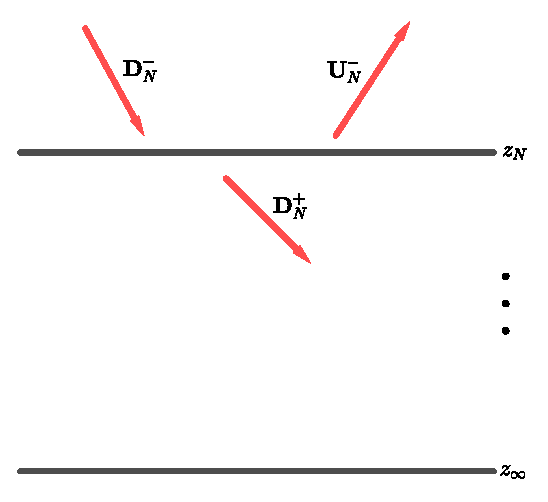
\includegraphics[scale=1]{ondas_em_zn}
\caption{\textit{Ondas ascendentes e descendentes na \'ultima interface.}}
\label{fig.ondas_em_zn}
\end{figure}

Substituindo a equa\c{c}\~ao \ref{eq.inversa_matriz_salto} na equa\c{c}\~ao anterior, temos
\begin{align*}
\begin{pmatrix}
\mathbf{U}_N^-\\
\mathbf{D}_N^-
\end{pmatrix}
&=
\begin{pmatrix}
J_{A,N}^\top&-J_{B,N}^\top\\
-J_{B,N}^\top&J_{A,N}^\top
\end{pmatrix}
\,
\begin{pmatrix}
0\\
\mathbf{D}_N^+
\end{pmatrix}\\\\
&=
\begin{pmatrix}
-J_{B,N}^\top \mathbf{D}_N^+\\
 J_{A,N}^\top \mathbf{D}_N^+
\end{pmatrix},
\end{align*}
ou seja,
\begin{align*}
\mathbf{U}_N^-&=-J_{B,N}^\top J_{A,N}^{-\top}\mathbf{D}_N^-\\
\mathbf{D}_N^+&=J_{A,N}^{-\top}\mathbf{D}_N^-.
\end{align*}
Assim, vemos que para computar uma onda refletida, ou seja, uma onda ascendente a partir de uma interface entre camadas, usamos uma \textit{matriz de reflex\~ao} que fica definida como
\begin{equation}\label{eq.reflexao_N}
\Gamma_N=-J_{B,N}^\top J_{A,N}^{-\top}.
\end{equation} 
Analogamente, vemos que para computar uma onda transmitida, ou seja, uma onda descendente a partir de uma interface entre camadas, usamos uma \textit{matriz de transmiss\~ao} que fica definida como
\begin{equation}\label{eq.transmissao_N}
T_N=J_{A,N}^{-\top}.
\end{equation} 

\subsection{Reflex\~ao e Transmiss\~ao numa Interface Qualquer}
Definimos a espessura de uma camada, a partir da interface superior, como
\begin{equation}
\Delta\,z_m=z_{m+1}-z_m,\qquad m=1,2,...,N-1,
\end{equation}
e temos que uma onda se propagando da interface na profundidade $z_m$ at\'e a interface em $z_{m+1}$ percorre uma profundidade total $\Delta\,z_m$. O valor dessa onda no fim da trajet\'oria, quando $z=z_{m+1}$, \'e aproximadamente igual a $\mathbf{\Psi}^-_{m+1}$, conforme a figura \ref{fig.N_interfaces}. Assim, usando a solu\c{c}\~ao \ref{eq.solucao_psi} podemos escrever
\begin{equation}\label{eq.solucao_delta_zm}
\mathbf{\Psi}^-_{m+1}=e^{-i\,\omega\tilde{\Lambda}_m\Delta\,z_m}\mathbf{\Psi}^+_m.
\end{equation}

\begin{figure}
\centering
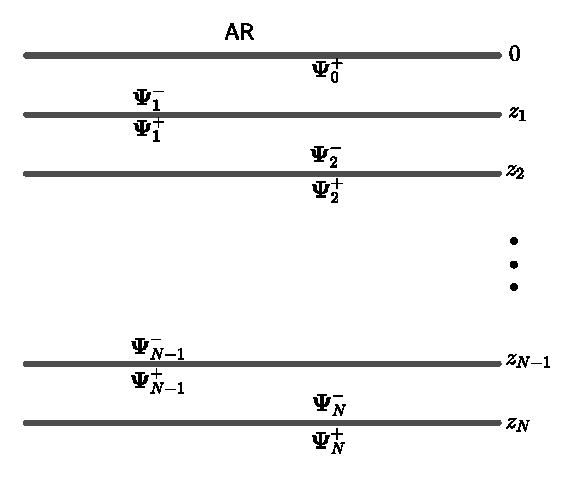
\includegraphics[scale=1]{n_interfaces}
\caption{\textit{Visualizacao de $N$ interfaces em subsuperficie e a notacao das ondas nas proximadades de cada interface.}}
\label{fig.N_interfaces}
\end{figure}

Sabendo que essa onda se propagando na camada abaixo da interface em $z_m$ veio da camada anterior, podemos usar a matriz de salto na equa\c{c}\~ao \ref{eq.psi_matriz_salto} e escrever
\begin{align}\label{eq.salto_m}
\mathbf{\Psi}^+_{m}&=J_m\,\mathbf{\Psi}^-_m.\\
\end{align}
Substituindo a equa\c{c}\~ao \ref{eq.salto_m} na equa\c{c}\~ao \ref{eq.solucao_delta_zm}, temos
\begin{align*}
\mathbf{\Psi}^-_{m+1}&=e^{-i\,\omega\tilde{\Lambda}_m\Delta\,z_m}\mathbf{\Psi}^+_m\\
\mathbf{\Psi}^-_{m+1}&=e^{-i\,\omega\tilde{\Lambda}_m\Delta\,z_m}J_m\,\mathbf{\Psi}^-_m\\
\mathbf{\Psi}^-_m&=J^{-1}_me^{i\,\omega\tilde{\Lambda}_m\Delta\,z_m}\mathbf{\Psi}^-_{m+1}
\end{align*}
Substituindo a equa\c{c}\~ao \ref{eq.definicao_psi} e a equa\c{c}\~ao \ref{eq.inversa_matriz_salto}, temos
\begin{align}\label{eq.refle_trans_1}
\mathbf{U}_m^-&=J^\top_{A,m}e^{i\,\omega\Lambda_m\Delta\,z_m}\mathbf{U}^-_{m+1}-J^\top_{B,m}e^{-i\,\omega\Lambda_m\Delta\,z_m}\mathbf{D}^-_{m+1}\\\nonumber\\\label{eq.refle_trans_2}
\mathbf{D}_m^-&=-J^\top_{B,m}e^{i\,\omega\Lambda_m\Delta\,z_m}\mathbf{U}^-_{m+1}+J^\top_{A,m}e^{-i\,\omega\Lambda_m\Delta\,z_m}\mathbf{D}^-_{m+1}.
\end{align}
Assim como definimos matriz de reflex\~ao para a \'ultima interface em $z_N$, podemos definir a matriz de reflex\~ao para uma interface qualquer, ou seja,
\begin{equation}\label{eq.reflexao_m+1}
\mathbf{U}^-_{m+1}=\Gamma_{m+1}\mathbf{D}^-_{m+1}.
\end{equation}
Substituindo a equa\c{c}\~ao \ref{eq.reflexao_m+1} na equa\c{c}\~ao \ref{eq.refle_trans_1} e na equa\c{c}\~ao \ref{eq.refle_trans_2}, temos
\begin{align}\label{eq.refle_trans_3}
\mathbf{U}_m^-&=(J^\top_{A,m}e^{i\,\omega\Lambda_m\Delta\,z_m}\Gamma_{m+1}-J^\top_{B,m}e^{-i\,\omega\Lambda_m\Delta\,z_m})\mathbf{D}^-_{m+1}\\\nonumber\\\label{eq.refle_trans_4}
\mathbf{D}_m^-&=(-J^\top_{B,m}e^{i\,\omega\Lambda_m\Delta\,z_m}\Gamma_{m+1}+J^\top_{A,m}e^{-i\,\omega\Lambda_m\Delta\,z_m})\mathbf{D}^-_{m+1}\,.
\end{align}
Substituindo a equa\c{c}\~ao \ref{eq.refle_trans_4} na equa\c{c}\~ao \ref{eq.refle_trans_3}, temos
\begin{align*}
\mathbf{U}_m^-&=(J^\top_{A,m}e^{i\,\omega\Lambda_m\Delta\,z_m}\Gamma_{m+1}-J^\top_{B,m}e^{-i\,\omega\Lambda_m\Delta\,z_m})\\
&\,\,\cdot\,\,(-J^\top_{B,m}e^{i\,\omega\Lambda_m\Delta\,z_m}\Gamma_{m+1}+J^\top_{A,m}e^{-i\,\omega\Lambda_m\Delta\,z_m})^{-1}\mathbf{D}_m^-\,,
\end{align*}
de onde podemos concluir que a matriz de reflex\~ao em uma interface em $z_m$ qualquer \'e dada por
\begin{align*}
\Gamma_{m}&=(J^\top_{A,m}e^{i\,\omega\Lambda_m\Delta\,z_m}\Gamma_{m+1}-J^\top_{B,m}e^{-i\,\omega\Lambda_m\Delta\,z_m})\\
&\,\,\cdot\,\,(-J^\top_{B,m}e^{i\,\omega\Lambda_m\Delta\,z_m}\Gamma_{m+1}+J^\top_{A,m}e^{-i\,\omega\Lambda_m\Delta\,z_m})^{-1},
\end{align*}
ou
\begin{align}\nonumber
\Gamma_{m}&=(J^\top_{A,m}e^{i\,\omega\Lambda_m\Delta\,z_m}\Gamma_{m+1}e^{i\,\omega\Lambda_m\Delta\,z_m}-J^\top_{B,m})\\\label{eq.matriz_reflexao_m}
&\,\,\cdot\,\,(-J^\top_{B,m}e^{i\,\omega\Lambda_m\Delta\,z_m}\Gamma_{m+1}e^{i\,\omega\Lambda_m\Delta\,z_m}+J^\top_{A,m})^{-1}.
\end{align}
Quando uma onda atinge uma interface, alem da possibilidade de reflexao ha tambem a possibilidade de trasmissao da onda para a camada inferior. De maneira analoga ao desenvolvido para reflexao de ondas, podemos deduzir a matriz para a transmissao de ondas em uma interface qualquer, que eh dada por
\begin{equation}\label{eq.matriz_transmissao_m}
T_m=T_{m+1}e^{i\,\omega\,\Lambda\Delta\,z_m}(-J^\top_{B,m}e^{i\,\omega\Lambda_m\Delta\,z_m}\Gamma_{m+1}e^{i\,\omega\Lambda_m\Delta\,z_m}+J^\top_{A,m})^{-1}.
\end{equation}
A validade das equacoes \ref{eq.matriz_reflexao_m} e \ref{eq.matriz_transmissao_m} para qualquer interface pode ser demonstrada por inducao sobre $m$, e todas as matrizes de reflexao e transmissao podem ser computadas por recurssao partindo das equacoes \ref{eq.reflexao_N} e \ref{eq.transmissao_N}.





mesclado
%\chapter{Solu\c{c}\~ao na Presen\c{c}a de Fonte}\label{sec.presenca_fonte}
Em porspec\c{c}\~ao de petr\'oleo s\~ao utilizadas alguns tipos de fontes de ondas, atrav\'es das quais se faz um mapeamento das caracter\'isticas das camadas de subsuperf\'icie. Esses tipos de fontes podem ser uma queda de peso, um caminh\~ao \textit{vibroseis}, explosivos e canh\~ao de ar, esta \'ultima fonte utilizada em prospec\c{c}\~ao mar\'itima. Sendo assim, vamos desenvolver uma solu\c{c}\~ao para o nosso problema considerando agora a presen\c{c}a de uma fonte.

Considere ainda a equa\c{c}\~ao \ref{eq.matricial} com o sobrescrito $m$ omitido. Uma fonte $\mathbf{S}$ localizada numa profundidade $z_s$ pode ser representada na forma
\begin{equation}\label{eq.fonte_geral}
\mathbf{S}=\mathbf{S}_0\delta(z-z_s)+\mathbf{S}_1\delta^\prime(z-z_s),
\end{equation}
onde $\mathbf{S}_0$ e $\mathbf{S}_1$ n\~ao dependem da profundidade e $\delta$ \'e a fun\c{c}ao \textit{Delta de Dirac}. Fontes que s\~ao distribu\'idas ao longo da profundidade podem, geralmente, ser sintetizadas por superposi\c{c}\~ao de fontes do tipo $\mathbf{S}_0$ e $\mathbf{S}_1$. 

Uma solu\c{c}\~ao por ser escrita como a combina\c{c}\~ao de uma solu\c{c}\~ao inicial sofrendo a a\c{c}\~ao de alguma fonte, ou seja,
\begin{equation}\label{eq.solucao_inicial_fonte}
\mathbf{\Phi}=\mathbf{\Phi}_0+\mathbf{S}_1\delta(z-z_s).
\end{equation} 
Substituindo a equa\c{c}\~ao \ref{eq.solucao_inicial_fonte} e a equa\c{c}\~ao \ref{eq.fonte_geral} na equa\c{c}\~ao \ref{eq.matricial}, temos
\begin{equation}\label{eq.matricial_fonte}
\frac{d\,\mathbf{\Phi}_0}{d\,z}=-i\,\omega\,M\,\mathbf{\Phi}_0+\left[\mathbf{S}_0-i\,\omega\,M\,\mathbf{S}_1\right]\,\delta(z-z_s),
\end{equation}
e por simplicidade, vamos escrever
\begin{equation}\label{eq.fonte_simplificada}
i\,\omega\,M\,\mathbf{S}_1-\mathbf{S}_0=
\begin{pmatrix}
\mathbf{S}_A\\
\mathbf{S}_B
\end{pmatrix}.
\end{equation}
Considerando a exist\^encia de uma interface imagin\'aria na profundidade $z_s$ da fonte, podemos determinar as condi\c{c}\~oes de salto no local da fonte da mesma forma que estudamos as condi\c{c}\~oes de salto nas interfaces que separam as camadas. Assim, integrando a equa\c{c}\~ao \ref{eq.matricial_fonte} no intervalo que come\c{c}a imediatamente acima da interface imagin\'aria da fonte $z_s^-$, e termina imediatamente abaixo da interface imagin\'aria da fonte em $z_s^+$, e substituindo a equa\c{c}\~ao \ref{eq.fonte_simplificada}, temos como solu\c{c}\~ao
\begin{equation*}
\mathbf{\Phi}_0(z_s^-)=\mathbf{\Phi}_0(z_s^+)+
\begin{pmatrix}
\mathbf{S}_A\\
\mathbf{S}_B
\end{pmatrix}.
\end{equation*}
Substituindo a equa\c{c}\~ao \ref{eq.solucao_inicial_fonte} e considerando as caracter\'isticas da fun\c{c}\~ao Delta de Dirac, temos a seguinte condi\c{c}\~ao de salto na profundidade da fonte
\begin{equation}\label{eq.salto_zs}
\mathbf{\Phi}(z_s^-)=\mathbf{\Phi}(z_s^+)+
\begin{pmatrix}
\mathbf{S}_A\\
\mathbf{S}_B
\end{pmatrix}.
\end{equation}

Vamos agora inserir uma interface imagin\'aria imediatamente abaixo da fonte, em $z=z_s^+$ e utilizar os m\'etodos do cap\'itulo \ref{sec.ausencia_fonte} para computar a matriz de reflex\~ao $\Gamma_s\equiv\Gamma(z_s^+)$ a partir do topo desta camada. J\'a que a interface em $z_s^+$ eh fict\'icia, as propriedades do meio s\~ao iguais acima e abaixo dessa interface, assim temos que $L_2^+=L_2^-$ e $L_1^+=L_1^-$. Substituindo essas identidades nas equa\c{c}\~oes \ref{eq.j_a} e \ref{eq.j_b}, temos
\begin{align}\label{eq.j_a_ficticia}
J_A&=\frac{1}{2}\left[(L_2)^\top L_1+(L_1)^\top L_2\right]\\\label{eq.j_b_ficticia}
J_B&=\frac{1}{2}\left[(L_2)^\top L_1-(L_1)^\top L_2\right].
\end{align}
Pela diagonaliza\c{c}\~ao de Ursin apresentada nas subse\c{c}\~oes \ref{sec.diagonalizacao_1}-\ref{sec.diagonalizacao_4}, conclu\'imos que 
\begin{align*}
L_1^\top&=L_2^{-1}\\
L_2^\top&=L_1^{-1},
\end{align*}
e substituindo as equa\c{c}\~oes acima nas equa\c{c}\~oes \ref{eq.j_a_ficticia} e \ref{eq.j_b_ficticia}, obtemos que
\begin{align*}
J_A&=I\\
J_B&=0.
\end{align*}
Desta forma, a onda ascendente $\mathbf{U}(z_s^+)$ e a onda descendente $\mathbf{D}(z_s^+)$ a partir da interface em $z_s^+$ podem ser introduzidas na equa\c{c}\~ao \ref{eq.definicao_psi} para obtermos
\begin{equation*}
\mathbf{\Psi}(z_s^+)=
\begin{pmatrix}
\mathbf{U}(z_s^+)\\
\mathbf{D}(z_s^+)
\end{pmatrix}.
\end{equation*}
Substituindo a equa\c{c}\~ao \ref{eq.reflexao_m+1} na equa\c{c}\~ao acima, temos
\begin{equation}\label{eq.Psi_descendente}
\mathbf{\Psi}(z_s^+)=
\begin{pmatrix}
\Gamma_s\mathbf{D}(z_s^+)\\
\mathbf{D}(z_s^+)
\end{pmatrix},
\end{equation}
pois as ondas est\~ao numa mesma camada e da\'i usamos que
\begin{align*}
\mathbf{U}^-(z_s^+)&=\mathbf{U}(z_s^+)\\
\mathbf{D}^-(z_s^+)&=\mathbf{D}(z_s^+).
\end{align*}
Multiplicando a equa\c{c}\~ao \ref{eq.salto_zs} por $L^{-1}$ e substituindo a equa\c{c}\~ao \ref{eq.Phi}, obtemos
\begin{equation}\label{eq.Psi_salto_zs}
\mathbf{\Psi}(z_s^-)=\mathbf{\Psi}(z_s^+)+L^{-1}
\begin{pmatrix}
\mathbf{S}_A\\
\mathbf{S}_B
\end{pmatrix}.
\end{equation}
Generalizando os desenvolvimentos apresentados nas subse\c{c}\~oes \ref{sec.diagonalizacao_1}-\ref{sec.diagonalizacao_4}, podemos escrever 
\begin{equation*}
L^{-1}=\frac{1}{\sqrt{2}}
\begin{pmatrix}
L_2^\top&L_1^\top\\
L_2^\top&-L_1^\top
\end{pmatrix},
\end{equation*}
e substituindo esta express\~ao para $L^{-1}$ juntamente com a equa\c{c}\~ao \ref{eq.Psi_descendente} na equa\c{c}\~ao \ref{eq.Psi_salto_zs}, temos
\begin{equation}\label{eq.solucao_phi_zs-}
\mathbf{\Psi}(z_s^-)=
\begin{pmatrix}
\Gamma_s\mathbf{D}(z_s^+)\\
\mathbf{D}(z_s^+)
\end{pmatrix}
+
\frac{1}{\sqrt{2}}\,
\begin{pmatrix}
L_2^\top\mathbf{S}_A+L_1^\top\mathbf{S}_B\\
L_2^\top\mathbf{S}_A-L_1^\top\mathbf{S}_B
\end{pmatrix}.
\end{equation}
Admitindo que a fonte esteja no interior da primeira camada, ou seja, $0<z_s<z_1$, a solu\c{c}\~ao dada pela equa\c{c}\~ao \ref{eq.solucao_phi_zs-} \'e propagada para cima a partir de $z_s^-$ usando a equa\c{c}\~ao \ref{eq.solucao_psi}, e o salto atrav\'es das interfaces entre camadas \'e dado pela equa\c{c}\~ao \ref{eq.psi_matriz_salto} at\'e que a onda atinja a interface terra/ar em $z=0^+$. Assim,
\begin{equation*}
\mathbf{\Psi}(0^+)=e^{-i\,\omega\,\tilde{\mathbf{\Lambda}}\,(0^+-z_s^-)}\,\mathbf{\Psi}(z_s^-),
\end{equation*}
e podemos usar as $n$ condi\c{c}\~oes de fronteira em $z=0$ para determinarmos as $n$ inc\'ognitas de $\mathbf{D}_s$. Os demais termos da solu\c{c}\~ao s\~ao conhecidos. A diferen\c{c}a $z_s^--0^+$ corresponde \`a profundidade da fonte, assim a solu\c{c}\~ao anterior pode ser reescrita como
\begin{align*}
\mathbf{\Psi}(0^+)&=e^{-i\,\omega\,\tilde{\mathbf{\Lambda}}\,(-z_s)}\,\mathbf{\Psi}(z_s^-)\\\\
\mathbf{\Psi}(0^+)&=
\begin{pmatrix}
e^{i\,\omega\,\mathbf{\Lambda}\,z_s}&\mathbf{0}\\
\mathbf{0}&e^{-i\,\omega\,\mathbf{\Lambda}\,z_s}
\end{pmatrix}
\mathbf{\Psi}(z_s^-).
\end{align*}
Substituindo a equa\c{c}\~ao \ref{eq.solucao_phi_zs-} na equa\c{c}\~ao acima, temos
\begin{equation}\label{eq.Psi_zero+}
\mathbf{\Psi}(0^+)=
\begin{pmatrix}
e^{i\,\omega\,\mathbf{\Lambda}\,z_s}\,\Gamma_s\mathbf{D}(z_s^+)\\
e^{-i\,\omega\,\mathbf{\Lambda}\,z_s}\,\mathbf{D}(z_s^+)
\end{pmatrix}
+
\frac{1}{\sqrt{2}}\,
\begin{pmatrix}
e^{i\,\omega\,\mathbf{\Lambda}\,z_s}\,(L_2^\top\mathbf{S}_A+L_1^\top\mathbf{S}_B)\\
e^{-i\,\omega\,\mathbf{\Lambda}\,z_s}\,(L_2^\top\mathbf{S}_A-L_1^\top\mathbf{S}_B)
\end{pmatrix}.
\end{equation}

TALVEZ SEJA INTERESSANTE COLOCAR A PARTE SEGUINTE NO CAPITULO ONDE SE DESENVOLVE AS EQUACOES MAIS PARTICULARES.

Para an\'alises futuras ser\'a interessante escrever a solu\c{c}\~ao na superf\'icie como
\begin{equation}\label{eq.Phi_G_AB}
\mathbf{\Phi}(0^+)=
\begin{pmatrix}
G_A\mathbf{\Phi}_g\\
G_B\mathbf{\Phi}_g
\end{pmatrix},
\end{equation}
onde as matrizes $G_A$ $G_B$ s\~ao de dimens\~ao $n\times n$ e $\mathbf{\Phi}_g$ \'e um vetor de dimens\~ao $n$ formado por inc\'ognitas em $z=0$.
Considerando o sistema \ref{eq.matricial_1}, temos
\begin{equation*}
\mathbf{\Phi}^{(1)}=
\begin{pmatrix}
\tilde{E}_1\\
\tilde{H}_2
\end{pmatrix}
\end{equation*}
e sua condi\c{c}\~ao de fronteira, quando $z=0$ \'e dada pela equa\c{c}\~ao \ref{eq.cond_fron_1}, 
\begin{equation*}
\tilde{H}_2=-\frac{\epsilon_0}{q_0}\tilde{E}_1.
\end{equation*}
Substituindo esta condi\c{c}\~ao em $\mathbf{\Phi}^{(1)}$, temos
\begin{equation*}
\mathbf{\Phi}^{(1)}=
\begin{pmatrix}
\tilde{E}_1\\\\
-\frac{\epsilon_0}{q_0}\tilde{E}_1
\end{pmatrix}_{z=0^+}.
\end{equation*}
Colocando a equa\c{c}\~ao acima no formato da equa\c{c}\~ao \ref{eq.Phi_G_AB}, temos que
\begin{equation*}
\mathbf{\Phi}_g^{(1)}=\tilde{E}_1,
\end{equation*}
\begin{equation*}
G_A^{(1)}=1\qquad\text{e}\qquad G_B^{(1)}=-\frac{\epsilon_0}{q_0}.
\end{equation*}
De maneira an\'aloga, vamos escrever as solu\c{c}\~oes dos tr\^es sistemas restantes na forma dada pela equa\c{c}\~ao \ref{eq.Phi_G_AB}. Substituindo a condi\c{c}\~ao de contorno \ref{eq.cond_fron_2} no sistema \ref{eq.matricial_2}, $\mathbf{\Phi}^{(2)}$ \'e dado por
\begin{equation*}
\mathbf{\Phi}^{(2)}=
\begin{pmatrix}
\tilde{E}_2\\\\
-\frac{q_0}{\mu_0}\tilde{E}_2
\end{pmatrix}_{z=0^+}
\end{equation*}
e temos
\begin{equation*}
\mathbf{\Phi}_g^{(2)}=\tilde{E}_2,
\end{equation*}
\begin{equation*}
G_A^{(2)}=1\qquad\text{e}\qquad G_B^{(2)}=-\frac{q_0}{\mu_0}.
\end{equation*}
Substituindo a condi\c{c}\~ao de contorno \ref{eq.cond_fron_3} no sistema \ref{eq.matricial_3}, $\mathbf{\Phi}^{(3)}$ \'e dado por
\begin{equation*}
\mathbf{\Phi}^{(3)}=
\begin{pmatrix}
\dot{\tilde{u}}_3\\
0\\
0\\
\dot{\tilde{u}}_1
\end{pmatrix}_{z=0^+}
\end{equation*}
e temos,
\begin{equation*}
\mathbf{\Phi}_g^{(3)}=
\begin{pmatrix}
\dot{\tilde{u}}_3\\
\dot{\tilde{u}}_1
\end{pmatrix},
\end{equation*}
\begin{equation*}
G_A^{(3)}=
\begin{pmatrix}
1&0\\
0&0
\end{pmatrix}
\qquad\text{e}\qquad G_B^{(3)}=
\begin{pmatrix}
0&0\\
0&1
\end{pmatrix}.
\end{equation*}

Substituindo a condi\c{c}\~ao de contorno \ref{eq.cond_fron_4} no sistema \ref{eq.matricial_4}, $\mathbf{\Phi}^{(4)}$ \'e dado por
\begin{equation*}
\mathbf{\Phi}^{(4)}=
\begin{pmatrix}
\dot{\tilde{u}}_2\\
0
\end{pmatrix}_{z=0^+}
\end{equation*}
e temos,
\begin{equation*}
\mathbf{\Phi}_g^{(4)}=\dot{\tilde{u}}_2,
\end{equation*}
\begin{equation*}
G_A^{(4)}=1\qquad\text{e}\qquad G_B^{(4)}=0.
\end{equation*}

De acordo com a equa\c{c}\~ao \ref{eq.Phi}, podemos escrever
\begin{equation*}
\mathbf{\Phi}(0^+)=L\,\mathbf{\Psi}(0^+),
\end{equation*}
e substituindo as equa\c{c}\~oes \ref{eq.Psi_zero+}, \ref{eq.Phi_G_AB} e \ref{eq.matriz_L} na equa\c{c}\~ao acima, temos
\begin{align}\label{eq.GA_Phi}
G_A\mathbf{\Phi}_g&=\frac{1}{\sqrt{2}}\,(L_1e^{i\,\omega\,\Lambda\,z_s}\Gamma_s\mathbf{D}_s+L_1e^{-i\,\omega\,\Lambda\,z_s}\mathbf{D}_s)\\\nonumber
&+\frac{1}{2}\,\left[L_1e^{i\,\omega\,\Lambda\,z_s}(L_2^\top\mathbf{S}_A+L_1^\top\mathbf{S}_B)+L_1e^{-i\,\omega\,\Lambda\,z_s}(L_2^\top\mathbf{S}_A-L_1^\top\mathbf{S}_B)\right]
\end{align}
e
\begin{align}\label{eq.GB_Phi}
G_B\mathbf{\Phi}_g&=\frac{1}{\sqrt{2}}\,(L_2e^{i\,\omega\,\Lambda\,z_s}\Gamma_s\mathbf{D}_s-L_2e^{-i\,\omega\,\Lambda\,z_s}\mathbf{D}_s)\\\nonumber
&+\frac{1}{2}\,\left[L_2e^{i\,\omega\,\Lambda\,z_s}(L_2^\top\mathbf{S}_A+L_1^\top\mathbf{S}_B)-L_2e^{-i\,\omega\,\Lambda\,z_s}(L_2^\top\mathbf{S}_A-L_1^\top\mathbf{S}_B)\right].
\end{align}
Pela diagonaliza\c{c}\~ao de Ursin podemos verificar que $L_1^\top=L_2^{-1}$, e multiplicando pela esquerda a equa\c{c}\~ao \ref{eq.GA_Phi} por $L_2^\top$ e multiplicando pela esquerda a equa\c{c}\~ao \ref{eq.GB_Phi} por $L_1^\top$, temos 
\begin{align}\label{eq.LGA_Phi}
L_2^{\top}G_A\mathbf{\Phi}_g&=\frac{1}{\sqrt{2}}\,(e^{i\,\omega\,\Lambda\,z_s}\Gamma_s\mathbf{D}_s+e^{-i\,\omega\,\Lambda\,z_s}\mathbf{D}_s)\\\nonumber
&+\frac{1}{2}\,\left[e^{i\,\omega\,\Lambda\,z_s}(L_2^\top\mathbf{S}_A+L_1^\top\mathbf{S}_B)+e^{-i\,\omega\,\Lambda\,z_s}(L_2^\top\mathbf{S}_A-L_1^\top\mathbf{S}_B)\right]
\end{align}
e
\begin{align}\label{eq.LGB_Phi}
L_1^\top G_B\mathbf{\Phi}_g&=\frac{1}{\sqrt{2}}\,(e^{i\,\omega\,\Lambda\,z_s}\Gamma_s\mathbf{D}_s-e^{-i\,\omega\,\Lambda\,z_s}\mathbf{D}_s)\\\nonumber
&+\frac{1}{2}\,\left[e^{i\,\omega\,\Lambda\,z_s}(L_2^\top\mathbf{S}_A+L_1^\top\mathbf{S}_B)-e^{-i\,\omega\,\Lambda\,z_s}(L_2^\top\mathbf{S}_A-L_1^\top\mathbf{S}_B)\right].
\end{align}
Subtraindo a equa\c{c}\~ao \ref{eq.LGB_Phi} da equa\c{c}\~ao \ref{eq.LGA_Phi}, temos
\begin{equation}\label{eq.pre_phi_g}
(L_2^{\top}G_A-L_1^\top G_B)\mathbf{\Phi}_g=\frac{2}{\sqrt{2}}\,e^{-i\,\omega\,\Lambda\,z_s}\mathbf{D}_s+e^{-i\,\omega\,\Lambda\,z_s}(L_2^\top\mathbf{S}_A-L_1^\top\mathbf{S}_B).
\end{equation}
Isolando $\mathbf{D}_s$ obtemos
\begin{equation*}
\mathbf{D}_s=\frac{1}{\sqrt{2}}\,e^{i\,\omega\,\Lambda\,z_s}(L_2^{\top}G_A-L_1^\top G_B)\,\mathbf{\Phi}_g-\frac{1}{\sqrt{2}}(L_2^\top\mathbf{S}_A-L_1^\top\mathbf{S}_B).
\end{equation*}
Ao multiplicar pela esquerda a equa\c{c}\~ao \ref{eq.pre_phi_g} por $e^{i\,\omega\,\Lambda\,z_s}\,\Gamma_se^{i\,\omega\,\Lambda\,z_s}$, temos
\begin{equation}\label{eq.pre_phi_g2}
e^{i\,\omega\,\Lambda\,z_s}\,\Gamma_se^{i\,\omega\,\Lambda\,z_s}(L_2^{\top}G_A-L_1^\top G_B)\mathbf{\Phi}_g=\frac{2}{\sqrt{2}}\,e^{i\,\omega\,\Lambda\,z_s}\,\Gamma_s\mathbf{D}_s+e^{i\,\omega\,\Lambda\,z_s}\,\Gamma_s(L_2^\top\mathbf{S}_A-L_1^\top\mathbf{S}_B),
\end{equation}
e somando as equa\c{c}\~oes \ref{eq.LGA_Phi} e \ref{eq.LGB_Phi}, temos
\begin{equation}\label{eq.pre_phi_g+}
(L_2^{\top}G_A+L_1^\top G_B)\mathbf{\Phi}_g=\frac{2}{\sqrt{2}}\,e^{i\,\omega\,\Lambda\,z_s}\Gamma_s\mathbf{D}_s+e^{i\,\omega\,\Lambda\,z_s}(L_2^\top\mathbf{S}_A+L_1^\top\mathbf{S}_B).
\end{equation}
Subtraindo a equa\c{c}\~ao \ref{eq.pre_phi_g+} da equa\c{c}\~ao \ref{eq.pre_phi_g2}, obtemos uma rela\c{c}\~ao para $\mathbf{\Phi}_g$, dada por 
\begin{align*}
\mathbf{\Phi}_g&=\left[e^{i\,\omega\,\Lambda\,z_s}\,\Gamma_se^{i\,\omega\,\Lambda\,z_s}(L_2^{\top}G_A-L_1^\top G_B)-(L_2^{\top}G_A+L_1^\top G_B)\right]^{-1}\\
&\,\,\cdot\,\,e^{i\,\omega\,\Lambda\,z_s}\left[\Gamma_s (L_2^\top\mathbf{S}_A-L_1^\top\mathbf{S}_B)-(L_2^\top\mathbf{S}_A+L_1^\top\mathbf{S}_B)\right].
\end{align*}
Em particular, quando a fonte est\'a imediatamente abaixo da superf\'icie livre, $z_s\approx0$, temos
\begin{equation*}
\mathbf{\Phi}_g=\left[(\Gamma_s-I)L_2^{\top}G_A-(\Gamma_s+I)L_1^\top G_B\right]^{-1}\left[(\Gamma_s-I)L_2^\top\mathbf{S}_A-(\Gamma_s+I)L_1^\top\mathbf{S}_B\right].
\end{equation*} 
Ap\'os obtermos $\mathbf{\Phi}_g$, \'e poss\'ivel determinarmos todas as condi\c{c}\~oes iniciais em $z=0$, $\mathbf{D}_s$ e $\mathbf{U}_s=\Gamma\,\mathbf{D}_s$. Em seguida, podemos obter a solu\c{c}\~ao imediatamente abaixo da fonte conforme a rela\c{c}\~ao \ref{eq.Psi_descendente}. Teoricamente, a partir de agora, a solu\c{c}\~ao pode ser computada em qualquer outra profundidade utilizando a propaga\c{c}\~ao atrav\'es das camadas de acordo com a rela\c{c}\~ao \ref{eq.solucao_psi} e o salto atrav\'es das camadas usando a rela\c{c}\~ao \ref{eq.psi_matriz_salto}. No entando, a propaga\c{c}\~ao de uma onda ascendente cont\'inua no sentido descendente \'e numericamente inst\'avel usando a equa\c{c}\~ao \ref{eq.solucao_psi}, pois as exponenciais complexas crescem ao inv\'es de diminuirem com a dist\^ancia. Assim, devemos obter $\mathbf{U}$ a partir de $\mathbf{D}$ usando $\Gamma_m$, ou fazer uso das matrizes de transmiss\~ao $T_m$.


mesclado
\chapter{Escrevendo as EDP's como um Sistema de EDO's}
Neste capitulo vamos aplicar algumas tecnicas como rotacao do sistema de coordenadas e Transformadas Laterais de Fourier em EDP's para que as mesmas possam ser escritas como um sistema de EDO's.

\section{Sistema de EDP's do Efeito Magnetoel\'astico}

Segundo \cite{eringen_1963}, o acoplamento entre ondas eletromagn\'eticas e el\'asticas se propagando no subsolo caracteriza o efeito magnetoel\'astico, e esse acoplamento pode ser modelado matematicamente atrav\'es de um sistema de equa\c{c}\~oes diferencias parciais. Conforme minha monografia, podemos aplicar uma s\'erie de hip\'oteses que visam simplificar e linearizar essas EDP's de forma que as mesmas possam receber um tratamento matem\'atico adequado no sentido de se obter numericamente os valores dos campos eletromagn\'eticos e el\'asticos envolvidos no sistema. Desta forma, vamos utilizar o m\'etodo matricial encontrado em \cite{Ursin-1983} na solu\c{c}\~ao do seguinte sistema de EDP's da magnetoelasticidade
\begin{align}\label{eq.mag_ela_1}
\nabla\times\mathbf{{E}}&=i\,\omega\,\mu_0\mathbf{{H}}\\\nonumber\\\label{eq.mag_ela_2}
\nabla\times\mathbf{{H}}&=(\sigma-i\,\epsilon\,\omega)\,\mathbf{{E}}+\mathbf{{v}}\times\sigma\mu_0\mathbf{H}^0\\\nonumber\\\label{eq.mag_ela_3}
-i\,\omega\rho\,\mathbf{{v}}&=\nabla\cdot{\tau} + \mathbf{{F}}\\\nonumber\\\label{eq.mag_ela_4}
{\tau}&=\lambda\,\nabla\cdot\mathbf{{u}}\cdot\,I + G\,(\nabla\,\mathbf{{u}}+\nabla\mathbf{{u}}^\top)\\\nonumber\\\label{eq.mag_ela_5}
\nabla\cdot\mathbf{{H}}&=0.
\end{align}
Estas equa\c{c}\~oes est\~ao no dom\'inio da frequ\^encia $\omega$, a depend\^encia do tempo \'e dada por $\exp{-i\,\omega\,t}$ e 
\begin{itemize}
\item $\mathbf{{E}}$ \'e o campo el\'etrico,
\item $\mathbf{{B}}$ \'e o campo magn\'etico,
\item $\mathbf{{D}}$ \'e o campo de densidade de fluxo el\'etrico,
\item $\mathbf{{H}}$ \'e o campo magn\'etico auxiliar,
\item $\tau$ \'e o tensor de tens\~oes,
\item $\mathbf{{u}}$ \'e o deslocamento do meio,
\item $\mathbf{{v}}$ \'e a velocidade de deslocamento do meio,
\item $\mathbf{{F}}$ \'e uma for\c{c}a aplicada ao meio,
\item $\mathbf{H}^0$ \'e campo geomagn\'etico,
\item $i$ \'e um n\'umero complexo,
\item $\omega$ \'e a frequ\^encia temporal,
\item $\mu_0$ \'e a permeabilidade magn\'etica no v\'acuo,
\item $\sigma$ \'e a condutividade do meio,
\item $\epsilon$ \'e a permissividade el\'etrica do meio,
\item $\rho$ \'e a densidade do meio,
\item $\lambda$ e $G$ s\~ao par\^ametros de Lam\`e.
\end{itemize}
Vamos definir $\sigma^*=(\sigma-i\,\epsilon\,\omega)$. No subsolo, por conta do regime quasi-estacion\'ario, $(\sigma>>\epsilon\,\omega)$  e  temos $\sigma^*=\sigma$. No ar, a condutividade \'e zero e a permeabilidade el\'etrica \'e pr\'oxima a do v\'acuo $\epsilon_0$, assim temos $\sigma^*=-i\,\epsilon_0\omega$.

No formato matricial, a equacao \ref{eq.mag_ela_1} pode ser escrita como
\begin{equation*}
\begin{pmatrix}
\frac{\partial\,E_3}{\partial\,y}-\frac{\partial\,E_2}{\partial\,z}\\
\frac{\partial\,E_1}{\partial\,z}-\frac{\partial\,E_3}{\partial\,x}\\
\frac{\partial\,E_2}{\partial\,x}-\frac{\partial\,E_1}{\partial\,y}
\end{pmatrix}
=
i\,\omega\,\mu_0\,
\begin{pmatrix}
H_1\\
H_2\\
H_3
\end{pmatrix}.
\end{equation*}
Aplicando as transformadas laterais de Fourier, dada em \ref{eq.trans_fourier_1}, temos
\begin{empheq}[left=\empheqlbrace]{align*}
-i\,k_y\widehat{E}_3-\frac{\partial\,\widehat{E}_2}{\partial\,z}&=i\,\omega\,\mu_0\widehat{H}_1\\
\frac{\partial\,\widehat{E}_1}{\partial\,z}+i\,k_x\widehat{E}_3&=i\,\omega\,\mu_0\widehat{H}_2\\
-i\,k_x\widehat{E}_2+i\,k_y\widehat{E}_1&=i\,\omega\,\mu_0\widehat{H}_3.
\end{empheq} 
Rotacionando o sistema de forma que a primeira coordenada esteja orientada no sentido do vetor de onda horizontal, usando o operador dado pela equacao \ref{eq.operador_rotacao}, e fazendo as simplificacoes, temos
\begin{empheq}[left=\empheqlbrace]{align*}
\frac{\partial\,\tilde{E}_2}{\partial\,z}&=-i\,\omega\,\mu_0\tilde{H}_1\\
\frac{\partial\,\tilde{E}_1}{\partial\,z}&=i\,\omega\,\mu_0\tilde{H}_2-i\,k\tilde{E}_3\\
\tilde{E}_2&=-\frac{\omega\,\mu_0}{k}\tilde{H}_3.
\end{empheq}

Observando que $\mathbf{v}=-i\,\omega\mathbf{u}$ depois de aplicada a transformada de Fourier no tempo, a equacao \ref{eq.mag_ela_2} pode ser escrita como
\begin{equation*}
\begin{pmatrix}
\frac{\partial\,H_3}{\partial\,y}-\frac{\partial\,H_2}{\partial\,z}\\
\frac{\partial\,H_1}{\partial\,z}-\frac{\partial\,H_3}{\partial\,x}\\
\frac{\partial\,H_2}{\partial\,x}-\frac{\partial\,H_1}{\partial\,y}
\end{pmatrix}
=
(\sigma-i\,\epsilon\,\omega)\,
\begin{pmatrix}
E_1\\
E_2\\
E_3
\end{pmatrix}
-i\,\omega\,
\begin{pmatrix}
u_2H_3^0-u_3H_2^0\\
u_3H_1^0-u_1H_3^0\\
u_1H_2^0-u_2H_1^0
\end{pmatrix}.
\end{equation*}
Aplicando as transformadas laterais de Fourier conforme a equacao \ref{eq.trans_fourier_1}, temos
\begin{empheq}[left=\empheqlbrace]{align*}
-i\,k_y\widehat{H}_3-\frac{\partial\,\widehat{H}_2}{\partial\,z}&=(\sigma-i\,\epsilon\,\omega)\,\widehat{E}_1-i\,\omega(u_2H_3^0-u_3H_2^0)\\
\frac{\partial\,\widehat{H}_1}{\partial\,z}+i\,k_x\widehat{H}_3&=(\sigma-i\,\epsilon\,\omega)\,\widehat{E}_2-i\,\omega(u_3H_1^0-u_1H_3)\\
-i\,k_x\widehat{H}_2+i\,k_y\widehat{H}_1&=(\sigma-i\,\epsilon\,\omega)\,\widehat{E}_3-i\,\omega(u_1H_2^0-u_2H_1^0).
\end{empheq}
Rotacionando o sistema usando o operador dado pela equacao \ref{eq.operador_rotacao}, e fazendo as simplificacoes, temos
\begin{empheq}[left=\empheqlbrace]{align*}
\frac{\partial\,\tilde{H}_2}{\partial\,z}&=-(\sigma-i\,\epsilon\,\omega)\,\tilde{E}_1+i\,\omega\,\tilde{H}_3^0\tilde{u}_2-i\,\omega\,\tilde{H}_2^0\tilde{u}_3\\
\frac{\partial\,\tilde{H}_1}{\partial\,z}&=(\sigma-i\,\epsilon\,\omega)\,\tilde{E}_2-i\,\omega\,k\,\tilde{H}_3-i\,\omega\,\tilde{H}_1^0\tilde{u}_3+i\,\omega\,\tilde{H}_3^0\tilde{u}_1\\
\tilde{H}_2&=-\frac{(\sigma-i\,\epsilon\,\omega)}{i\,k}\tilde{E}_3+\frac{\omega}{k}  \tilde{H}_2^0\tilde{u}_1-\frac{\omega}{k}\tilde{H}_1^0\tilde{u}_2.
\end{empheq}

A equacao \ref{eq.mag_ela_3} pode ser reescrita como

\begin{empheq}[left=\empheqlbrace]{align*}
-\omega^2\rho\,u_1&=\frac{\partial \tau_{11}}{\partial\,x}+\frac{\partial \tau_{12}}{\partial\,y}+\frac{\partial \tau_{13}}{\partial\,z}+F_1\\
-\omega^2\rho\,u_2&=\frac{\partial \tau_{21}}{\partial\,x}+\frac{\partial \tau_{22}}{\partial\,y}+\frac{\partial \tau_{23}}{\partial\,z}+F_2\\
-\omega^2\rho\,u_3&=\frac{\partial \tau_{31}}{\partial\,x}+\frac{\partial \tau_{32}}{\partial\,y}+\frac{\partial \tau_{33}}{\partial\,z}+F_3
\end{empheq}
Aplicando as transformadas laterais de Fourier, temos
\begin{empheq}[left=\empheqlbrace]{align*}
-\omega^2\rho\,\widehat{u}_1&=-i\,k_x\widehat{\tau}_{11}-i\,k_y\widehat{\tau}_{12}+\frac{\partial\widehat{\tau}_{13}}{\partial\,z}+\widehat{F}_1\\
-\omega^2\rho\,\widehat{u}_2&=-i\,k_x\widehat{\tau}_{21}-i\,k_y\widehat{\tau}_{22}+\frac{\partial\widehat{\tau}_{23}}{\partial\,z}+\widehat{F}_2\\
-\omega^2\rho\,\widehat{u}_3&=-i\,k_x\widehat{\tau}_{31}-i\,k_y\widehat{\tau}_{32}+\frac{\partial\widehat{\tau}_{33}}{\partial\,z}+\widehat{F}_3.
\end{empheq}
Aplicando a rotacao e simplificando as equacoes, temos
\begin{empheq}[left=\empheqlbrace]{align*}
-\omega^2\rho\,\tilde{u}_1&=-i\,k\tilde{\tau}_{11}+\frac{\partial\tilde{\tau}_{13}}{\partial\,z}+\tilde{F}_1\\
-\omega^2\rho\,\tilde{u}_2&=-i\,k\tilde{\tau}_{12}+\frac{\partial\tilde{\tau}_{23}}{\partial\,z}+\tilde{F}_2\\
-\omega^2\rho\,\tilde{u}_3&=-i\,k\tilde{\tau}_{13}+\frac{\partial\tilde{\tau}_{33}}{\partial\,z}+\tilde{F}_3.
\end{empheq}


\chapter{Condi\c{c}\~oes de Contorno do Efeito Magneto-El\'astico e o Espa\c{c}o Original}

Como estamos assumindo que as propriedades materiais n\~ao se alteram no interior de cada camada da subsuperf\'icie, temos que a matriz $M^{(m)}$ \'e constante para cada camada. Essas propriedades materiais se alteram descontinuamente conforme $z$ varia de uma camada para outra atrav\'es da interface de contato entre as camadas. Nessas interfaces vamos aplicar as condi\c{c}\~oes de interface encontradas em \cite{pride_94}, onde o vetor $\mathbf{u}$, as componentes normais de $\tau$ e as componentes  tangenciais de $\mathbf{E}$ e $\mathbf{H}$ s\~ao cont\'inuas. Assim, constatamos que os vetores $\mathbf{\Phi}^{(m)}$ s\~ao cont\'inuos atrav\'es das interfaces entre as camadas.

\section{Condi\c{c}\~oes de Contorno}
Resta estabelecer condi\c{c}\~oes de contorno para os sistemas \ref{eq.matricial_1}-\ref{eq.matricial_4} no contato ar/superf\'icie, ou seja, em $z=0$. Aplicando ainda as condi\c{c}\~oes de interface encontradas em \cite{pride_94}, temos que a condi\c{c}\~ao de contorno para o sistema \ref{eq.matricial_1} \'e
\begin{equation}\label{eq.cond_fron_1}
\tilde{H}_2=-\frac{\epsilon_0}{q_0}\tilde{E}_1,
\end{equation}
onde $q_0$ \'e a vagarosidade vertical dada por \ref{eq.vagarosidade_vertical}. Esta \'e a rela\c{c}\~ao para uma onda eletromagn\'etica ascendente, e foi deduzida do fato de que n\~ao h\'a ondas eletromagn\'eticas descendentes no ar, pois todas a fontes est\~ao na subsuperf\'icie.
Para o sistema \ref{eq.matricial_2}, a condi\c{c}\~ao de contorno \'e
\begin{equation}\label{eq.cond_fron_2}
\tilde{H}_1=\frac{q_0}{\mu_0}\tilde{E}_2,
\end{equation}
onde esta rela\c{c}\~ao tamb\'em foi deduzida do fato de que h\'a apenas ondas eletromagn\'eticas ascendentes no ar.
Para o sistema \ref{eq.matricial_3}, as condi\c{c}\~oes de contorno s\~ao
\begin{equation}\label{eq.cond_fron_3}
\tilde{\tau}_{13}=\tilde{\tau}_{33}=0.
\end{equation}
E para o sistema \ref{eq.matricial_4}, a condi\c{c}\~ao de contorno \'e
\begin{equation}\label{eq.cond_fron_4}
\tilde{\tau}_{23}=0.
\end{equation}
Observe que para cada um dos sistemas, precisaremos de condi\c{c}\~oes de contorno adicionais para especificar uma solu\c{c}\~ao. Essas condi\c{c}\~oes surgir\~ao, por ocasi\~ao da aplica\c{c}\~ao nas equa\c{c}\~oes da magneto-elasticidade, do fato de que n\~ao h\'a ondas ascendentes em $z\rightarrow\infty$, como pudemos observar na subse\c{c}\~ao \ref{sec.ausencia_fonte} e na figura \ref{fig.ondas_em_zn}.

Essas condi\c{c}\~oes de contorno s\~ao utilizadas nas equa\c{c}\~oes da magneto-elasticidade mas podem desde j\'a serem inseridas na solu\c{c}\~ao gen\'erica apresentada na subse\c{c}\~ao \ref{sec.presenca_fonte}, como foi desenvolvido por v\'arios autores como \cite{White_Zhou_2006}, \cite{Azeredo_2013}, \cite{miranda_2016} e \cite{oliveira_2018}. Tal abordagem \'e interessante por facilitar an\'alises futuras, assim, vamos escrever a solu\c{c}\~ao na superf\'icie como
\begin{equation}\label{eq.Phi_G_AB}
\mathbf{\Phi}(0^+)=
\begin{pmatrix}
G_A\mathbf{\Phi}_g\\
G_B\mathbf{\Phi}_g
\end{pmatrix},
\end{equation}
onde as matrizes $G_A$ $G_B$ s\~ao de dimens\~ao $n\times n$ e $\mathbf{\Phi}_g$ \'e um vetor de dimens\~ao $n$ formado por inc\'ognitas em $z=0$.
Considerando o sistema \ref{eq.matricial_1}, temos
\begin{equation*}
\mathbf{\Phi}^{(1)}=
\begin{pmatrix}
\tilde{E}_1\\
\tilde{H}_2
\end{pmatrix}
\end{equation*}
e sua condi\c{c}\~ao de fronteira, quando $z=0$ \'e dada pela equa\c{c}\~ao \ref{eq.cond_fron_1}, 
\begin{equation*}
\tilde{H}_2=-\frac{\epsilon_0}{q_0}\tilde{E}_1.
\end{equation*}
Substituindo esta condi\c{c}\~ao em $\mathbf{\Phi}^{(1)}$, temos
\begin{equation*}
\mathbf{\Phi}^{(1)}=
\begin{pmatrix}
\tilde{E}_1\\\\
-\frac{\epsilon_0}{q_0}\tilde{E}_1
\end{pmatrix}_{z=0^+}.
\end{equation*}
Colocando a equa\c{c}\~ao acima no formato da equa\c{c}\~ao \ref{eq.Phi_G_AB}, temos que
\begin{equation*}
\mathbf{\Phi}_g^{(1)}=\tilde{E}_1,
\end{equation*}
\begin{equation*}
G_A^{(1)}=1\qquad\text{e}\qquad G_B^{(1)}=-\frac{\epsilon_0}{q_0}.
\end{equation*}
De maneira an\'aloga, vamos escrever as solu\c{c}\~oes dos tr\^es sistemas restantes na forma dada pela equa\c{c}\~ao \ref{eq.Phi_G_AB}. Substituindo a condi\c{c}\~ao de contorno \ref{eq.cond_fron_2} no sistema \ref{eq.matricial_2}, $\mathbf{\Phi}^{(2)}$ \'e dado por
\begin{equation*}
\mathbf{\Phi}^{(2)}=
\begin{pmatrix}
\tilde{E}_2\\\\
-\frac{q_0}{\mu_0}\tilde{E}_2
\end{pmatrix}_{z=0^+}
\end{equation*}
e temos
\begin{equation*}
\mathbf{\Phi}_g^{(2)}=\tilde{E}_2,
\end{equation*}
\begin{equation*}
G_A^{(2)}=1\qquad\text{e}\qquad G_B^{(2)}=-\frac{q_0}{\mu_0}.
\end{equation*}
Substituindo a condi\c{c}\~ao de contorno \ref{eq.cond_fron_3} no sistema \ref{eq.matricial_3}, $\mathbf{\Phi}^{(3)}$ \'e dado por
\begin{equation*}
\mathbf{\Phi}^{(3)}=
\begin{pmatrix}
\dot{\tilde{u}}_3\\
0\\
0\\
\dot{\tilde{u}}_1
\end{pmatrix}_{z=0^+}
\end{equation*}
e temos,
\begin{equation*}
\mathbf{\Phi}_g^{(3)}=
\begin{pmatrix}
\dot{\tilde{u}}_3\\
\dot{\tilde{u}}_1
\end{pmatrix},
\end{equation*}
\begin{equation*}
G_A^{(3)}=
\begin{pmatrix}
1&0\\
0&0
\end{pmatrix}
\qquad\text{e}\qquad G_B^{(3)}=
\begin{pmatrix}
0&0\\
0&1
\end{pmatrix}.
\end{equation*}

Substituindo a condi\c{c}\~ao de contorno \ref{eq.cond_fron_4} no sistema \ref{eq.matricial_4}, $\mathbf{\Phi}^{(4)}$ \'e dado por
\begin{equation*}
\mathbf{\Phi}^{(4)}=
\begin{pmatrix}
\dot{\tilde{u}}_2\\
0
\end{pmatrix}_{z=0^+}
\end{equation*}
e temos,
\begin{equation*}
\mathbf{\Phi}_g^{(4)}=\dot{\tilde{u}}_2,
\end{equation*}
\begin{equation*}
G_A^{(4)}=1\qquad\text{e}\qquad G_B^{(4)}=0.
\end{equation*}

De acordo com a equa\c{c}\~ao \ref{eq.Phi}, podemos escrever
\begin{equation*}
\mathbf{\Phi}(0^+)=L\,\mathbf{\Psi}(0^+),
\end{equation*}
e substituindo as equa\c{c}\~oes \ref{eq.Psi_zero+}, \ref{eq.Phi_G_AB} e \ref{eq.matriz_L} na equa\c{c}\~ao acima, temos
\begin{align}\label{eq.GA_Phi}
G_A\mathbf{\Phi}_g&=\frac{1}{\sqrt{2}}\,(L_1e^{i\,\omega\,\Lambda\,z_s}\Gamma_s\mathbf{D}_s+L_1e^{-i\,\omega\,\Lambda\,z_s}\mathbf{D}_s)\\\nonumber
&+\frac{1}{2}\,\left[L_1e^{i\,\omega\,\Lambda\,z_s}(L_2^\top\mathbf{S}_A+L_1^\top\mathbf{S}_B)+L_1e^{-i\,\omega\,\Lambda\,z_s}(L_2^\top\mathbf{S}_A-L_1^\top\mathbf{S}_B)\right]
\end{align}
e
\begin{align}\label{eq.GB_Phi}
G_B\mathbf{\Phi}_g&=\frac{1}{\sqrt{2}}\,(L_2e^{i\,\omega\,\Lambda\,z_s}\Gamma_s\mathbf{D}_s-L_2e^{-i\,\omega\,\Lambda\,z_s}\mathbf{D}_s)\\\nonumber
&+\frac{1}{2}\,\left[L_2e^{i\,\omega\,\Lambda\,z_s}(L_2^\top\mathbf{S}_A+L_1^\top\mathbf{S}_B)-L_2e^{-i\,\omega\,\Lambda\,z_s}(L_2^\top\mathbf{S}_A-L_1^\top\mathbf{S}_B)\right].
\end{align}
Utilizando novamente as equa\c{c}\~oes \ref{eq.l1l2} e \ref{eq.l2l1}, podemos multiplicar pela esquerda a equa\c{c}\~ao \ref{eq.GA_Phi} por $L_2^\top$ e multiplicar pela esquerda a equa\c{c}\~ao \ref{eq.GB_Phi} por $L_1^\top$, deduzindo que
\begin{align}\label{eq.LGA_Phi}
L_2^{\top}G_A\mathbf{\Phi}_g&=\frac{1}{\sqrt{2}}\,(e^{i\,\omega\,\Lambda\,z_s}\Gamma_s\mathbf{D}_s+e^{-i\,\omega\,\Lambda\,z_s}\mathbf{D}_s)\\\nonumber
&+\frac{1}{2}\,\left[e^{i\,\omega\,\Lambda\,z_s}(L_2^\top\mathbf{S}_A+L_1^\top\mathbf{S}_B)+e^{-i\,\omega\,\Lambda\,z_s}(L_2^\top\mathbf{S}_A-L_1^\top\mathbf{S}_B)\right]
\end{align}
e
\begin{align}\label{eq.LGB_Phi}
L_1^\top G_B\mathbf{\Phi}_g&=\frac{1}{\sqrt{2}}\,(e^{i\,\omega\,\Lambda\,z_s}\Gamma_s\mathbf{D}_s-e^{-i\,\omega\,\Lambda\,z_s}\mathbf{D}_s)\\\nonumber
&+\frac{1}{2}\,\left[e^{i\,\omega\,\Lambda\,z_s}(L_2^\top\mathbf{S}_A+L_1^\top\mathbf{S}_B)-e^{-i\,\omega\,\Lambda\,z_s}(L_2^\top\mathbf{S}_A-L_1^\top\mathbf{S}_B)\right].
\end{align}
Subtraindo a equa\c{c}\~ao \ref{eq.LGB_Phi} da equa\c{c}\~ao \ref{eq.LGA_Phi}, temos
\begin{equation}\label{eq.pre_phi_g}
(L_2^{\top}G_A-L_1^\top G_B)\mathbf{\Phi}_g=\frac{2}{\sqrt{2}}\,e^{-i\,\omega\,\Lambda\,z_s}\mathbf{D}_s+e^{-i\,\omega\,\Lambda\,z_s}(L_2^\top\mathbf{S}_A-L_1^\top\mathbf{S}_B),
\end{equation}
E isolando $\mathbf{D}_s$ obtemos
\begin{equation*}
\mathbf{D}_s=\frac{1}{\sqrt{2}}\,e^{i\,\omega\,\Lambda\,z_s}(L_2^{\top}G_A-L_1^\top G_B)\,\mathbf{\Phi}_g-\frac{1}{\sqrt{2}}(L_2^\top\mathbf{S}_A-L_1^\top\mathbf{S}_B).
\end{equation*}
Ao multiplicar pela esquerda a equa\c{c}\~ao \ref{eq.pre_phi_g} por $e^{i\,\omega\,\Lambda\,z_s}\,\Gamma_se^{i\,\omega\,\Lambda\,z_s}$, temos
\begin{equation}\label{eq.pre_phi_g2}
e^{i\,\omega\,\Lambda\,z_s}\,\Gamma_se^{i\,\omega\,\Lambda\,z_s}(L_2^{\top}G_A-L_1^\top G_B)\mathbf{\Phi}_g=\frac{2}{\sqrt{2}}\,e^{i\,\omega\,\Lambda\,z_s}\,\Gamma_s\mathbf{D}_s+e^{i\,\omega\,\Lambda\,z_s}\,\Gamma_s(L_2^\top\mathbf{S}_A-L_1^\top\mathbf{S}_B),
\end{equation}
e somando as equa\c{c}\~oes \ref{eq.LGA_Phi} e \ref{eq.LGB_Phi}, temos
\begin{equation}\label{eq.pre_phi_g+}
(L_2^{\top}G_A+L_1^\top G_B)\mathbf{\Phi}_g=\frac{2}{\sqrt{2}}\,e^{i\,\omega\,\Lambda\,z_s}\Gamma_s\mathbf{D}_s+e^{i\,\omega\,\Lambda\,z_s}(L_2^\top\mathbf{S}_A+L_1^\top\mathbf{S}_B).
\end{equation}
Subtraindo a equa\c{c}\~ao \ref{eq.pre_phi_g+} da equa\c{c}\~ao \ref{eq.pre_phi_g2}, obtemos uma rela\c{c}\~ao para $\mathbf{\Phi}_g$, dada por 
\begin{align*}
\mathbf{\Phi}_g&=\left[e^{i\,\omega\,\Lambda\,z_s}\,\Gamma_se^{i\,\omega\,\Lambda\,z_s}(L_2^{\top}G_A-L_1^\top G_B)-(L_2^{\top}G_A+L_1^\top G_B)\right]^{-1}\\
&\,\,\cdot\,\,e^{i\,\omega\,\Lambda\,z_s}\left[\Gamma_s (L_2^\top\mathbf{S}_A-L_1^\top\mathbf{S}_B)-(L_2^\top\mathbf{S}_A+L_1^\top\mathbf{S}_B)\right].
\end{align*}
Em particular, quando a fonte est\'a imediatamente abaixo da superf\'icie livre, $z_s\approx0$, temos
\begin{equation*}
\mathbf{\Phi}_g=\left[(\Gamma_s-I)L_2^{\top}G_A-(\Gamma_s+I)L_1^\top G_B\right]^{-1}\left[(\Gamma_s-I)L_2^\top\mathbf{S}_A-(\Gamma_s+I)L_1^\top\mathbf{S}_B\right].
\end{equation*} 
Ap\'os obtermos $\mathbf{\Phi}_g$, \'e poss\'ivel determinarmos todas as condi\c{c}\~oes iniciais em $z=0$, $\mathbf{D}_s$ e $\mathbf{U}_s=\Gamma\,\mathbf{D}_s$. Em seguida, podemos obter a solu\c{c}\~ao imediatamente abaixo da fonte conforme a rela\c{c}\~ao \ref{eq.Psi_descendente}. Teoricamente, a partir de agora, a solu\c{c}\~ao pode ser computada em qualquer outra profundidade utilizando a propaga\c{c}\~ao atrav\'es das camadas de acordo com a rela\c{c}\~ao \ref{eq.solucao_psi} e o salto atrav\'es das camadas usando a rela\c{c}\~ao \ref{eq.psi_matriz_salto}. No entanto, segundo \cite{White_Zhou_2006}, a propaga\c{c}\~ao de uma onda ascendente cont\'inua no sentido descendente \'e numericamente inst\'avel usando a equa\c{c}\~ao \ref{eq.solucao_psi}, pois as exponenciais complexas crescem ao inv\'es de diminuirem com a dist\^ancia. Assim, devemos obter $\mathbf{U}$ a partir de $\mathbf{D}$ usando $\Gamma_m$, ou fazer uso das matrizes de transmiss\~ao $T_m$.

\section{Solu\c{c}\~ao no Espa\c{c}o Original}

No processo de estabelecimento das EDP's do efeito magneto-el\'astico encontrado em \cite{pinho_2018}, a transformada de Fourier foi aplicada \`as equa\c{c}\~oes para que as mesmas fossem escritas no dom\'inio da frequ\^encia temporal. Aqui nesta monografia, aplicamos as transformadas laterais de Fourier deixando somente as derivadas em rela\c{c}\~ao \`a profundidade, para em seguida aplicar uma mudan\c{c}a de eixos coordenados, atrav\'es de uma rota\c{c}\~ao, facilitando a manipula\c{c}\~ao alg\'ebrica das equa\c{c}\~oes. Para obtermos as solu\c{c}\~oes no espa\c{c}o original, \'e necess\'ario aplicarmos os procedimentos que invertem esses procedimentos aplicados anteriormente.

\subsection{Rota\c{c}\~ao Inversa}
No cap\'itulo \ref{sec.trans_edp_2_edo}, os campos vetoriais foram rotacionados utilizando a rela\c{c}\~ao \ref{eq.operador_rotacao}, assim vamos obter os campos no sistema de coordenadas anterior aplicando a rela\c{c}\~ao \ref{eq.rotacao_inversa}. 


Para o campo el\'etrico, temos
\begin{equation*}
\dot{\hat{E}}_1=\frac{k_x}{k}\dot{\tilde{E}}_1-\frac{k_y}{k}\dot{\tilde{E}}_2\qquad
\dot{\hat{E}}_2=\frac{k_y}{k}\dot{\tilde{E}}_1+\frac{k_x}{k}\dot{\tilde{E}}_2\qquad
\dot{\hat{E}}_3=\dot{\tilde{E}}_3.
\end{equation*}


Para o campo magn\'etico auxiliar,
\begin{equation*}
\dot{\hat{H}}_1=\frac{k_x}{k}\dot{\tilde{H}}_1-\frac{k_y}{k}\dot{\tilde{H}}_2\qquad
\dot{\hat{H}}_2=\frac{k_y}{k}\dot{\tilde{H}}_1+\frac{k_x}{k}\dot{\tilde{H}}_2\qquad
\dot{\hat{H}}_3=\dot{\tilde{H}}_3.
\end{equation*}


Para velocidade de deslocamento do meio temos
\begin{equation*}
\dot{\hat{u}}_1=\frac{k_x}{k}\dot{\tilde{u}}_1-\frac{k_y}{k}\dot{\tilde{u}}_2\qquad
\dot{\hat{u}}_2=\frac{k_y}{k}\dot{\tilde{u}}_1+\frac{k_x}{k}\dot{\tilde{u}}_2\qquad
\dot{\hat{u}}_3=\dot{\tilde{u}}_3.
\end{equation*}

Para o tensor de tens\~oes vamos aplicar a rota\c{c}\~ao inversa dada pela equa\c{c}\~ao \ref{eq.rot_inver_tensor},\\
\begin{minipage}{.5\textwidth}
\begin{align*}
\hat{\tau}_{11}&=\frac{k_x^2}{k^2}\tilde{\tau}_{11}-2\frac{k_xk_y}{k^2}\tilde{\tau}_{12}+\frac{k_y^2}{k^2}\tilde{\tau}_{22}\\\\
\hat{\tau}_{12}&=\frac{k_xk_y}{k^2}(\tilde{\tau}_{11}-\tilde{\tau}_{22})+\left(\frac{k_x^2-k_y^2}{k^2}\tilde{\tau}_{12}\right)\\\\
\hat{\tau}_{22}&=\frac{k_y^2}{k^2}\tilde{\tau}_{11}+2\frac{k_xk_y}{k^2}\tilde{\tau}_{12}+\frac{k_x^2}{k^2}\tilde{\tau}_{22}
\end{align*}
\end{minipage}
\begin{minipage}{.5\textwidth}
\begin{align*}
\hat{\tau}_{13}&=\frac{k_x}{k}\tilde{\tau}_{13}-\frac{k_y}{k}\tilde{\tau}_{23}\\\\
\hat{\tau}_{23}&=\frac{k_y}{k}\tilde{\tau}_{13}+\frac{k_x}{k}\tilde{\tau}_{23}\\\\
\hat{\tau}_{33}&=\tilde{\tau}_{33}.
\end{align*}
\end{minipage}\\


As rela\c{c}\~oes acima podem ser simplificadas dependendo do tipo de fonte de onda s\'ismica utilizada.


\subsection{Transformada de Hankel e Transformada Lateral de Fourier}

Agora devemos inverter a transformada lateral de Fourier usando a rela\c{c}\~ao \ref{eq.trans_fourier_2} para obtermos as solu\c{c}\~oes no espa\c{c}o real. Observe que as matrizes das equa\c{c}\~oes \ref{eq.matricial_1} a \ref{eq.matricial_4} dependem somente da vagarosidade $\gamma$, ou da magnitude $k$ do vetor $(k_x,k_y)^\top$ e n\~ao da dire\c{c}\~ao desse vetor. No entanto, fatores contendo $k_x$ e $k_y$ foram introduzidos pela transformada dada pela rela\c{c}\~ao \ref{eq.trans_fourier_1}. Assim, para aplicar a transformada lateral inversa de Fourier de forma pr\'atica, vamos utilizar a seguinte rela\c{c}\~ao onde $\hat{g}(k)$ \'e uma fun\c{c}\~ao qualquer e $m_1$ e $m_2$ s\~ao inteiros positivos, 
\begin{equation}\label{eq.transf_auxiliar}
\Theta_{m_1,m_2}[k_x^{m_1}\,k_y^{m_2}\,\hat{g}(k)]=(-i)^{m_1+m_2}\left(\frac{\partial}{\partial\,x}\right)^{m_1}\left(\frac{\partial}{\partial\,y}\right)^{m_2}\frac{1}{2\,\pi}\int_{\mathbb{R}}\hat{g}(k)\,e^{i\,k}\,dk.
\end{equation}
Escrevendo as coordenadas cartesianas como coordenadas cil\'indricas, temos
\begin{equation}
x_1=r\,\cos\theta\qquad x_2=r\,\text{sen}\theta\qquad x_3=z,
\end{equation}
e podemos calcular a transformada dada pela equa\c{c}\~ao \ref{eq.transf_auxiliar} atrav\'es da transformada inversa de Hankel, descrita na subse\c{c}\~ao \ref{sec.trans_hankel}. Considere
\begin{equation}\label{eq.trans_hankel_adapt}
\mathcal{B}[\hat{g}(k)]=\frac{1}{2\,\pi}\int_0^\infty k^{m_1}J_{m_2}(k\,r)\hat{g}(k)\,dk,
\end{equation}
onde $J_{m_2}$ \'e uma fun\c{c}\~ao de Bessel dada pela equa\c{c}\~ao \ref{eq.funcao_bessel_2}, e para os casos particulares onde $m_1,m_2\,\in[0,3]$, temos\\
\begin{minipage}{.5\textwidth}
\begin{align*}
\Theta_{0,0}&=\mathcal{B}_{1,0}\\
\Theta_{2,0}&=\cos^2\theta\mathcal{B}_{3,0}-\frac{\cos^2\theta-\text{sen}^2\theta}{r}\mathcal{B}_{2,1}\\
\Theta_{0,1}&=i\,\text{sen}\theta\mathcal{B}_{2,1}
\end{align*}
\end{minipage}
\begin{minipage}{.5\textwidth}
\begin{align*}
\Theta_{1,1}&=\text{sen}\theta\,\cos\theta\left[\mathcal{B}_{3,0}-\frac{2}{r}\mathcal{B}_{2,1}\right]\\
\Theta_{1,0}&=i\,\cos\theta\mathcal{B}_{2,1}\\
\Theta_{0,2}&=\text{sen}^2\theta\mathcal{B}_{3,0}+\frac{\cos^2\theta-\text{sen}^2\theta}{r}\mathcal{B}_{2,1}
\end{align*}
\end{minipage}






\chapter{Aplicando a Diagonaliza\c{c}\~ao de Ursin}\label{sec.diagonalizacao_ursin}

%\section{Introdu\c{c}\~ao}
   

\section{Aplicando a Diagonaliza\c{c}\~ao de Ursin na Equa\c{c}\~ao \ref{eq.matricial_1}}\label{sec.diagonalizacao_1}

Comparando a equa\c{c}\~ao \ref{eq.matricial_1} com a equa\c{c}\~ao \ref{eq.matricial} vemos que as matrizes
\begin{equation*}
M^{(1)}_1=\frac{-\mu_0\sigma-i\,\gamma^2\omega}{\overline{\sigma}}\qquad\text{e}\qquad\,M^{(1)}_2=\frac{\overline{\sigma}}{i\,\omega}.
\end{equation*}
Definimos autovalores e autovetores relacionados ao operador $M^{(1)}_1\cdot M^{(1)}_2$ na forma 
\begin{equation}\label{eq.def_auto_1}
\frac{-\mu_0\sigma-i\,\gamma^2\omega}{\overline{\sigma}}\cdot\frac{\overline{\sigma}}{i\,\omega}\,\mathbf{a}^{(1)}={q^{(1)}}^2\mathbf{a}^{(1)},
\end{equation}
e para termos um autovetor n\~ao trivial, \'e necess\'ario o autovalor
\begin{equation*}
q^{(1)}=\sqrt{\frac{-\mu_0\sigma-i\,\gamma^2\omega}{i\,\omega}}.
\end{equation*}
Substituindo o autovalor acima na equa\c{c}\~ao \ref{eq.def_auto_1}, temos que o autovetor $\mathbf{a}^{(1)}$ \'e o autoespa\c{c}o relativo ao autovalor $q^{(1)}$ e ${1}$ \'e uma base para esse autoespa\c{c}o.\\
O autovetor relacionado ao operador $M^{(1)}_2\cdot M^{(1)}_1$ \'e dado por
\begin{equation*}
\mathbf{b}^{(1)}=\frac{\overline{\sigma}}{i\,\omega\,\sqrt{\frac{-\mu_0\sigma-i\,\gamma^2\omega}{i\,\omega}}}\cdot\mathbf{a}^{(1)}.
\end{equation*}
Tomando arbitrariamente o valor $\mathbf{a}^{(1)}=1$ temos que as submatrizes de diagonaliza\c{c}\~ao s\~ao
\begin{equation*}
L^{(1)}_1=1\qquad\text{e}\qquad L^{(1)}_2=\frac{\overline{\sigma}}{i\,\omega\,\sqrt{\frac{-\mu_0\sigma-i\,\gamma^2\omega}{i\,\omega}}},
\end{equation*}
e as matrizes para diagonaliza\c{c}\~ao s\~ao dadas por
\begingroup
\Large
\begin{align*}
L^{(1)}&=\frac{1}{\sqrt{2}}\,
\begin{pmatrix}
1&1\\
\frac{\overline{\sigma}}{i\,\omega\,\sqrt{\frac{-\mu_0\sigma-i\,\gamma^2\omega}{i\,\omega}}}&-\frac{\overline{\sigma}}{i\,\omega\,\sqrt{\frac{-\mu_0\sigma-i\,\gamma^2\omega}{i\,\omega}}}
\end{pmatrix}\\\\
{L^{(1)}}^{-1}&=\frac{1}{\sqrt{2}}\,
\begin{pmatrix}
1&\frac{i\,\omega\,\sqrt{\frac{-\mu_0\sigma-i\,\gamma^2\omega}{i\,\omega}}}{\overline{\sigma}}\\
1&-\frac{i\,\omega\,\sqrt{\frac{-\mu_0\sigma-i\,\gamma^2\omega}{i\,\omega}}}{\overline{\sigma}}
\end{pmatrix}.
\end{align*}
\endgroup
A matriz semelhante a $M^{(1)}$ \'e
\begin{equation*}
\tilde{\Lambda}^{(1)}=
\begin{pmatrix}
\sqrt{\frac{-\mu_0\sigma-i\,\gamma^2\omega}{i\,\omega}}&0\\
0&-\sqrt{\frac{-\mu_0\sigma-i\,\gamma^2\omega}{i\,\omega}}
\end{pmatrix}.
\end{equation*}

\section{Aplicando a Diagonaliza\c{c}\~ao de Ursin na Equa\c{c}\~ao \ref{eq.matricial_2}}\label{sec.diagonalizacao_2}

Comparando a equa\c{c}\~ao \ref{eq.matricial_2} com a equa\c{c}\~ao \ref{eq.matricial} vemos que as matrizes
\begin{equation*}
M^{(2)}_1=-\mu_0\qquad\text{e}\qquad\,M^{(2)}_2=\frac{\overline{\sigma}\,\mu_0+i\,\omega\,\gamma^2}{i\,\omega\,\mu_0}.
\end{equation*}
Definimos autovalores e autovetores relacionados ao operador $M^{(2)}_1\cdot M^{(2)}_2$ na forma
\begin{equation}\label{eq.def_auto_2}
-\mu_0\cdot\frac{\overline{\sigma}\,\mu_0+i\,\omega\,\gamma^2}{i\,\omega\,\mu_0}\,\mathbf{a}^{(2)}={q^{(2)}}^2\mathbf{a}^{(2)},
\end{equation}
e para termos um autovetor n\~ao trivial, \'e necess\'ario o autovalor
\begin{equation*}
q^{(2)}=\sqrt{-\frac{\overline{\sigma}\,\mu_0+i\,\omega\,\gamma^2}{i\,\omega}}.
\end{equation*}
Substituindo o autovalor $q^{(2)}$ na equa\c{c}\~ao \ref{eq.def_auto_2}, temos que o autovetor $\mathbf{a}^{(2)}$ \'e o autoespa\c{c}o relativo ao autovalor $q^{(2)}$ e ${1}$ \'e uma base para esse autoespa\c{c}o.\\
O autovetor relacionado ao operador $M^{(2)}_2\cdot M^{(2)}_1$ \'e dado por
\begin{equation*}
\mathbf{b}^{(2)}=-\frac{1}{\mu_0}\,\sqrt{-\frac{\overline{\sigma}\,\mu_0+i\,\omega\,\gamma^2}{i\,\omega}}\cdot\mathbf{a}^{(2)}.
\end{equation*}
Tomando arbitrariamente o valor $\mathbf{a}^{(2)}=1$ temos que as submatrizes de diagonaliza\c{c}\~ao s\~ao
\begin{equation*}
L^{(2)}_1=1\qquad\text{e}\qquad L^{(2)}_2=-\frac{1}{\mu_0}\,\sqrt{-\frac{\overline{\sigma}\,\mu_0+i\,\omega\,\gamma^2}{i\,\omega}},
\end{equation*}
e as matrizes para diagonaliza\c{c}\~ao s\~ao dadas por
\begin{Large}
\begin{align*}
L^{(2)}&=\frac{1}{\sqrt{2}}\,
\begin{pmatrix}
1&1\\
-\frac{1}{\mu_0}\,\sqrt{-\frac{\overline{\sigma}\,\mu_0+i\,\omega\,\gamma^2}{i\,\omega}}&\frac{1}{\mu_0}\,\sqrt{-\frac{\overline{\sigma}\,\mu_0+i\,\omega\,\gamma^2}{i\,\omega}}
\end{pmatrix}\\\\
{L^{(2)}}^{-1}&=\frac{1}{\sqrt{2}}\,
\begin{pmatrix}
1&-\mu_0\,(-\frac{\overline{\sigma}\,\mu_0+i\,\omega\,\gamma^2}{i\,\omega})^{-\frac{1}{2}}\\
1&\mu_0\,(-\frac{\overline{\sigma}\,\mu_0+i\,\omega\,\gamma^2}{i\,\omega})^{-\frac{1}{2}}
\end{pmatrix}.
\end{align*}
\end{Large}
A matriz semelhante a $M^{(2)}$ \'e
\begin{equation*}
\tilde{\Lambda}^{(2)}=
\begin{pmatrix}
\sqrt{-\frac{\overline{\sigma}\,\mu_0+i\,\omega\,\gamma^2}{i\,\omega}}&0\\
0&-\sqrt{-\frac{\overline{\sigma}\,\mu_0+i\,\omega\,\gamma^2}{i\,\omega}}
\end{pmatrix}.
\end{equation*}

\section{Aplicando a Diagonaliza\c{c}\~ao de Ursin na Equa\c{c}\~ao \ref{eq.matricial_3}}\label{sec.diagonalizacao_3}

Comparando a equa\c{c}\~ao \ref{eq.matricial_3} com a equa\c{c}\~ao \ref{eq.matricial} vemos que as matrizes
\begin{equation*}
M^{(3)}_1=
\begin{pmatrix}
\beta&\lambda\,\gamma\,\beta\\
\lambda\,\gamma\,\beta&\rho+\gamma^2\beta(\lambda^2-\beta^{-1})
\end{pmatrix}
\quad\text{e}\quad
M^{(3)}_2=
\begin{pmatrix}
\rho&\gamma\\
\gamma&G^{-1}
\end{pmatrix}
\end{equation*}
onde definimos $\beta=\frac{1}{\lambda+2\,G}$.\\
Definimos autovalores e autovetores relacionados ao operador $M^{(3)}_1\cdot M^{(3)}_2$ na forma
\begin{equation*}
\begin{pmatrix}
\beta&\lambda\,\gamma\,\beta\\
\lambda\,\gamma\,\beta&\rho+\gamma^2\beta(\lambda^2-\beta^{-1})
\end{pmatrix}
\cdot
\begin{pmatrix}
\rho&\gamma\\
\gamma&G^{-1}
\end{pmatrix}
\,\mathbf{a}^{(3)}_i
=
{q^{(3)}_i}^2\mathbf{a}^{(3)}_i,
\end{equation*}
para $i=1,2$.  E para evitarmos solu\c{c}\~oes triviais, \'e necess\'ario que seja nulo o determinante da matriz
\begin{equation}\label{eq.def_auto_3}
\begin{pmatrix}
\beta\,\rho+\lambda\,\gamma^2\beta-{q^{(3)}_i}^2&\beta\,\gamma+\lambda\,\gamma\,\beta\,G^{-1}\\
\lambda\,\gamma\,\beta\,\rho+\rho\,\gamma+\gamma^3\beta\,(\lambda^2-\beta^{-2})&\lambda\,\gamma^2\beta+\frac{\rho+\gamma^2\beta\,(\lambda^2-\beta^{-2})}{G}-{q^{(3)}_i}^2
\end{pmatrix}
\begin{pmatrix}
a_{i\,1}\\
a_{i\,2}
\end{pmatrix}
=
\begin{pmatrix}
0\\
0
\end{pmatrix}.
\end{equation}
Anulando o determinante da matriz acima chegamos \`a equa\c{c}\~ao do segundo grau em ${q^{(3)}_i}^2$
\begin{equation*}
\begin{split}
{q^{(3)}_i}^4-\left(\beta\,\rho+2\,\lambda\,\gamma^2\beta+\frac{\rho+\gamma^2\beta\,(\lambda^2-\beta^{-2})}{G}\right)\,{q^{(3)}_i}^2\\\\
-\left(\beta\,\gamma+\lambda\,\gamma\,\beta\,G^{-1}\right)\left[\lambda\,\gamma\,\beta\,\rho+\rho\,\gamma+\gamma^3\beta\,(\lambda^2-\beta^{-2})\right]\\\\
+(\beta\,\rho+\lambda\,\gamma^2\beta)\left[\lambda\,\gamma^2\beta+\frac{\rho+\gamma^2\beta\,(\lambda^2-\beta^{-2})}{G}\right]=0.
\end{split}
\end{equation*}
Os autovalores ${q^{(3)}_1}^2$ e ${q^{(3)}_2}^2$ s\~ao dados, respectivamente, tomando o sinal positivo e o sinal negativo antes da radicia\c{c}\~ao na equa\c{c}\~ao
\begin{equation*}
{q^{(3)}_i}^2=\frac{1}{2}\,\left[\beta\,\rho+2\,\lambda\,\gamma^2\beta+\frac{\rho+\gamma^2\beta\,(\lambda^2-\beta^{-2})}{G}\right]\pm\frac{1}{2}\sqrt{\Delta},
\end{equation*}
onde $\Delta$ \'e dado por
\begin{align*}
\Delta&=
\left[\beta\,\rho+2\,\lambda\,\gamma^2\beta+\frac{\rho+\gamma^2\beta\,(\lambda^2-\beta^{-2})}{G}\right]^2\\\\
&-4\,(\beta\,\rho+\lambda\,\gamma^2\beta)\left[\lambda\,\gamma^2\beta+\frac{\rho+\gamma^2\beta\,(\lambda^2-\beta^{-2})}{G}\right]\\\\
&+4\,\left(\beta\,\gamma+\lambda\,\gamma\,\beta\,G^{-1}\right)\left[\lambda\,\gamma\,\beta\,\rho+\rho\,\gamma+\gamma^3\beta\,(\lambda^2-\beta^{-2})\right].
\end{align*}
Como ${q^{(3)}_i}^2$ foi deduzido de forma que a matriz na equa\c{c}\~ao \ref{eq.def_auto_3} tenha determinante nulo, temos que as linhas dessa matriz s\~ao linearmente dependentes. Assim, vamos utilizar a linha 1 para definir os autovetores
\begin{equation*}
a_{i1}=-\frac{\beta\,\gamma+\lambda\,\gamma\,\beta\,G^{-1}}{\beta\,\rho+\lambda\,\gamma^2\beta-{q^{(3)}_i}^2}\,a_{i2},
\end{equation*}
onde $a_{i2}\in \mathbb{C}$. Por quest\~ao de facilidade de escrita, dentro do autoespa\c{c}o definido pela equa\c{c}\~ao acima, vamos escolher $a_{i2}=\beta\,\rho+\lambda\,\gamma^2\beta-{q^{(3)}_i}^2$, e os autovetores relacionados ao operador $M^{(3)}_1\cdot M^{(3)}_2$ s\~ao
\begin{equation*}
\mathbf{a}^{(3)}_1
=
\begin{pmatrix}
-\beta\,\gamma+\lambda\,\gamma\,\beta\,G^{-1}\\
\beta\,\rho+\lambda\,\gamma^2\beta-{q^{(3)}_1}^2
\end{pmatrix}
\quad\text{e}\quad
\mathbf{a}^{(3)}_2
=
\begin{pmatrix}
-\beta\,\gamma+\lambda\,\gamma\,\beta\,G^{-1}\\
\beta\,\rho+\lambda\,\gamma^2\beta-{q^{(3)}_2}^2
\end{pmatrix}.
\end{equation*}
Os autovetores relacionados ao operador $M^{(3)}_2\cdot M^{(3)}_1$ s\~ao dados por
\begin{align*}
\mathbf{b}^{(3)}_1
&=
\frac{1}{{q^{(3)}_1}}
\begin{pmatrix}
-\rho\,(\beta\,\gamma+\lambda\,\gamma\,\beta\,G^{-1})+\gamma\,(\beta\,\rho+\lambda\,\gamma^2\beta-{q^{(3)}_1}^2)\\
-\gamma\,(\beta\,\gamma+\lambda\,\gamma\,\beta\,G^{-1})+G^{-1}(\beta\,\rho+\lambda\,\gamma^2\beta-{q^{(3)}_1}^2)
\end{pmatrix}\\\\
\mathbf{b}^{(3)}_2
&=
\frac{1}{{q^{(3)}_2}}
\begin{pmatrix}
-\rho\,(\beta\,\gamma+\lambda\,\gamma\,\beta\,G^{-1})+\gamma\,(\beta\,\rho+\lambda\,\gamma^2\beta-{q^{(3)}_2}^2)\\
-\gamma\,(\beta\,\gamma+\lambda\,\gamma\,\beta\,G^{-1})+G^{-1}(\beta\,\rho+\lambda\,\gamma^2\beta-{q^{(3)}_2}^2)
\end{pmatrix}.
\end{align*}
Usando os autovetores, temos que as submatrizes de diagonaliza\c{c}\~ao s\~ao
\begin{equation*}
L^{(3)}_1=
\begin{pmatrix}
\mathbf{a}^{(3)}_1&\mathbf{a}^{(3)}_2
\end{pmatrix}
\quad\text{e}\quad
L^{(3)}_2=
\begin{pmatrix}
\mathbf{b}^{(3)}_1&\mathbf{b}^{(3)}_2
\end{pmatrix},
\end{equation*}
e as matrizes para diagonaliza\c{c}\~ao s\~ao dadas por
\begin{align*}
L^{(3)}&=\frac{1}{\sqrt{2}}
\begin{pmatrix}
\mathbf{a}^{(3)}_1&\mathbf{a}^{(3)}_2&\mathbf{a}^{(3)}_1&\mathbf{a}^{(3)}_2\\
\mathbf{b}^{(3)}_1&\mathbf{b}^{(3)}_2&-\mathbf{b}^{(3)}_1&-\mathbf{b}^{(3)}_2
\end{pmatrix}
\quad\text{e}
\\\\
{L^{(3)}}^{-1}&=\frac{1}{\sqrt{2}}
\begin{pmatrix}
{\mathbf{b}^{(3)}_1}^{\top}&{\mathbf{a}^{(3)}_1}^{\top}\\
{\mathbf{b}^{(3)}_2}^{\top}&{\mathbf{a}^{(3)}_2}^{\top}\\
{\mathbf{b}^{(3)}_1}^{\top}&-{\mathbf{a}^{(3)}_1}^{\top}\\
{\mathbf{b}^{(3)}_2}^{\top}&-{\mathbf{a}^{(3)}_2}^{\top}
\end{pmatrix}.
\end{align*}
A matriz semelhante a $M^{(3)}$ \'e
\begin{equation*}
\tilde{\Lambda}^{(3)}=
\begin{pmatrix}
q^{(3)}_1&0&0&0\\
0&q^{(3)}_2&0&0\\
0&0&-q^{(3)}_1&0\\
0&0&0&-q^{(3)}_2
\end{pmatrix}.
\end{equation*}


\section{Aplicando a Diagonaliza\c{c}\~ao de Ursin na Equa\c{c}\~ao \ref{eq.matricial_4}}\label{sec.diagonalizacao_4}

Comparando a equa\c{c}\~ao \ref{eq.matricial_4} com a equa\c{c}\~ao \ref{eq.matricial} vemos que as matrizes
\begin{equation*}
M^{(4)}_1=G^{-1}\qquad\text{e}\qquad\,M^{(4)}_2=\rho-G\,\gamma^2.
\end{equation*}
Definimos autovalores e autovetores relacionados ao operador $M^{(4)}_1\cdot M^{(4)}_2$ na forma
\begin{equation}\label{eq.def_auto_4}
G^{-1}(\rho-G\,\gamma^2)\,\mathbf{a}^{(4)}={q^{(4)}}^2\mathbf{a}^{(4)},
\end{equation}
e para termos um autovetor n\~ao trivial, \'e necess\'ario o autovalor
\begin{equation*}
{q^{(4)}}^2=G^{-1}(\rho-G\,\gamma^2).
\end{equation*}
Substituindo o autovalor ${q^{(4)}}^2$ na equa\c{c}\~ao \ref{eq.def_auto_4}, temos que o autovetor $\mathbf{a}^{(4)}$ \'e o autoespa\c{c}o relativo ao autovalor ${q^{(4)}}^2$ e ${1}$ \'e uma base para esse autoespa\c{c}o.\\
O autovetor relacionado ao operador $M^{(4)}_2\cdot M^{(4)}_1$ \'e dado por
\begin{equation*}
\mathbf{b}^{(4)}=[G\,(\rho-G\,\gamma^2)]^{\frac{1}{2}}   \cdot\mathbf{a}^{(4)}.
\end{equation*}
Tomando arbitrariamente o valor $\mathbf{a}^{(4)}=1$ temos que as submatrizes de diagonaliza\c{c}\~ao s\~ao
\begin{equation*}
L^{(4)}_1=1\qquad\text{e}\qquad L^{(4)}_2=[G\,(\rho-G\,\gamma^2)]^{\frac{1}{2}},
\end{equation*}
e as matrizes para diagonaliza\c{c}\~ao s\~ao dadas por
\begin{align*}
L^{(4)}&=\frac{1}{\sqrt{2}}\,
\begin{pmatrix}
1&1\\
[G\,(\rho-G\,\gamma^2)]^{\frac{1}{2}}&-[G\,(\rho-G\,\gamma^2)]^{\frac{1}{2}}
\end{pmatrix}\\\\
{L^{(4)}}^{-1}&=\frac{1}{\sqrt{2}}\,
\begin{pmatrix}
1&[G\,(\rho-G\,\gamma^2)]^{-\frac{1}{2}}\\
1&-[G\,(\rho-G\,\gamma^2)]^{-\frac{1}{2}}
\end{pmatrix}.
\end{align*}
A matriz semelhante a $M^{(4)}$ \'e
\begin{equation*}
\tilde{\Lambda}^{(4)}=
\begin{pmatrix}
[G^{-1}(\rho-G\,\gamma^2)]^{\frac{1}{2}}&0\\
0&-[G^{-1}(\rho-G\,\gamma^2)]^{\frac{1}{2}}
\end{pmatrix}.
\end{equation*}





%\section{Decomposi\c{c}\~ao em Ondas Ascendentes e Descentes}
%
%Para realizar a decomposi\c{c}\~ao do vetor $\mathbf{B}$ em ondas ascendentes e descendentes aplicamos uma diagonaliza\c{c}\~ao em autovalores na matriz $A$ na forma
%\begin{equation}\label{eq.diagonalizacao}
%A=L\,\Lambda_1L^{-1}\,,
%\end{equation}
%onde $\Lambda_1$ \'e a matriz diagonal dos autovalores $\lambda_i$ para $i=1,2,...,n$, e $L$ \'e a matriz dos autovetores correspondentes,
%\begin{equation}\label{eq.Lambda_1}
%\Lambda_1=
%\begin{bmatrix}
%\Lambda&0\\
%0&-\Lambda
%\end{bmatrix}\,.
%\end{equation} 
%A defini\c{c}\~ao de autovalores e autovetores \'e dada por
%\begin{equation}\label{eq.sist_autovalores}
%\begin{bmatrix}
%0&A_1\\
%A_2&0
%\end{bmatrix}
%\begin{bmatrix}
%\mathbf{L_1}\\
%\mathbf{L_2}
%\end{bmatrix}
%=
%\lambda\,
%\begin{bmatrix}
%\mathbf{L_1}\\
%\mathbf{L_2}
%\end{bmatrix}
%\end{equation}
%e aplicando o procedimento
%\begin{equation*}
%\begin{bmatrix}
%0&A_1\\
%A_2&0
%\end{bmatrix}
%\begin{bmatrix}
%0&A_1\\
%A_2&0
%\end{bmatrix}
%\begin{bmatrix}
%\mathbf{L_1}\\
%\mathbf{L_2}
%\end{bmatrix}
%=
%\lambda\,\lambda\,
%\begin{bmatrix}
%\mathbf{L_1}\\
%\mathbf{L_2}
%\end{bmatrix}\,,
%\end{equation*}
%podemos separar o sitema \ref{eq.sist_autovalores} de dimens\~ao $2n$ em dois sistemas de dimens\~ao n
%\begin{align*}
%A_1A_2\mathbf{L_1}&=\lambda^2\mathbf{L_1}\\
%A_2A_1\mathbf{L_2}&=\lambda^2\mathbf{L_2}\,,
%\end{align*}
%onde $\mathbf{L}_i$ s\~ao os vetores que, concatenados dois a dois, formam os autovetores que comp\~oem $L$.
%Assim, podemos dividir a diagonaliza\c{c}\~ao dada em \ref{eq.diagonalizacao} em duas diagonaliza\c{c}\~oes de dimens\~ao $n$
%\begin{align}\label{eq.subdiagonalizacao}\nonumber
%A_1A_2&=L_1\Lambda^2L_1^{-1}\\\quad\\\nonumber
%A_2A_1&=L_2\Lambda^2L_2^{-1}\,,
%\end{align}
%onde $L_i$ s\~ao submatrizes da matriz $L$ e cont\^em os autovetores $\mathbf{L}_i$.
%
%
%
%Definindo a matriz 
%\begin{equation}\label{eq.L}
%L=\frac{1}{\sqrt{2}}
%\begin{bmatrix}
%L_1&L_1\\
%L_2&-L_2
%\end{bmatrix}
%\end{equation}
%e sua inversa
%\begin{equation}\label{eq.L_inversa}
%L^{-1}=\frac{1}{\sqrt{2}}
%\begin{bmatrix}
%L_1^{-1}&L_2^{-1}\\
%L_1^{-1}&-L_2^{-1}
%\end{bmatrix}\,,
%\end{equation}
%podemos substitu\'i-las na equa\c{c}\~ao \ref{eq.diagonalizacao} e verificar que 
%\begin{align}\label{eq.definicao_A1_A2}\nonumber
%A_1&=L_1\Lambda\,L_2^{-1}\\\quad\\\nonumber
%A_2&=L_2\Lambda\,L_1^{-1}\,,
%\end{align}
%e podemos verificar ainda que essas defini\c{c}\~oes para $A_1$ e $A_2$ satisfazem tamb\'em as equa\c{c}\~oes \ref{eq.subdiagonalizacao}.
%
%Pelas caracter\'isticas da equa\c{c}\~ao \ref{eq.matricial} sabemos que as matrizes $A_1$ e $A_2$ s\~ao sim\'etricas e podem ser escritas como
%\begin{align*}
%A_1&=L_2^{-\top}\Lambda\,L_1^\top\\
%A_2&=L_1^{-\top}\Lambda\,L_2^\top\,,
%\end{align*}
%as quais substitu\'idas nas equa\c{c}\~oes \ref{eq.subdiagonalizacao} lucramos
%\begin{equation*}
%A_1A_2=L_1\Lambda^2L_1^{-1}=L_2^{-\top}\Lambda^2L_2^\top\,,
%\end{equation*}
%e conclu\'imos que, a menos da escala dos autovetores,
%\begin{equation*}
%L_1=L_2^{-\top}\,.
%\end{equation*}
%Substituindo a \'ultima igualdade na defini\c{c}\~ao \ref{eq.definicao_A1_A2} temos
%\begin{equation*}
%A_i=L_i\Lambda\,L_i^{\top}\qquad\text{para}\qquad i=1\,\text{e}\,2\,,
%\end{equation*}
%e substituindo em \ref{eq.L_inversa}, temos
%\begin{equation}\label{eq.L_inversa_2}
%L^{-1}=\frac{1}{\sqrt{2}}
%\begin{bmatrix}
%L_2^{\top}&L_1^{\top}\\
%L_2^{\top}&-L_1^{\top}
%\end{bmatrix}\,.
%\end{equation}
%
%Escrevendo o vetor de ondas na forma
%\begin{equation}\label{eq.transformacao_B}
%\mathbf{B}=L\,\mathbf{W}\,,
%\end{equation}
%aplicando a derivada parcial em rela\c{c}\~ao a $z$, e substituindo as equa\c{c}\~oes \ref{eq.matricial} e \ref{eq.diagonalizacao}, obtemos
%\begin{equation}\label{eq.derivada_W}
%\frac{\partial\mathbf{W}}{\partial\,z}=\left[\pm i\omega\,\Lambda_1-L^{-1}\frac{\partial\,L}{\partial\,z}\right]\,\mathbf{W}\,.
%\end{equation}
%Para a propaga\c{c}\~ao de ondas em camadas homog\^eneas, os coeficientes das EDP's originais s\~ao constantes por camada e esses coeficientes comp\~oem a matriz $A$ diagonalizada pela matriz $L$. Assim, para meios homog\^eneos, a \'ultima equa\c{c}\~ao pode ser reduzida a
%\begin{equation*}
%\frac{\partial\mathbf{W}}{\partial\,z}=\pm i\omega\,\Lambda_1\mathbf{W}\,.
%\end{equation*}
%Representamos o vetor $\mathbf{W}$ como
%\begin{equation*}
%\mathbf{W}=
%\begin{bmatrix}
%\mathbf{U}\\
%\mathbf{D}
%\end{bmatrix}\,,
%\end{equation*}
%onde $\mathbf{U}$ e $\mathbf{D}$ s\~ao vetores que representam ondas ascendentes e descendentes, respectivamente, desde que a parte real de $\pm i\omega\lambda_i$ seja n\~ao negativa para $i=1,2,...,n$.
%
%Substiutindo as equa\c{c}\~oes \ref{eq.L} e \ref{eq.L_inversa_2} na equa\c{c}\~ao \ref{eq.derivada_W} e efetuando as multiplica\c{c}\~oes matriciais obtemos
%\begin{align}\label{eq.Up_Down}\nonumber
%\frac{\partial\mathbf{U}}{\partial z}&=\pm i\omega\,\Lambda\,\mathbf{U}+F\,\mathbf{U}+G\,\mathbf{D}\\\quad\\\nonumber
%\frac{\partial\mathbf{D}}{\partial z}&=\pm i\omega\,\Lambda\,\mathbf{D}+F\,\mathbf{D}+G\,\mathbf{U}
%\end{align}
%onde as matrizes $F$ e $G$ s\~ao, respectivamente,
%\begin{align*}
%F&=-\frac{1}{2}\left[L_2^\top\frac{\partial L_1}{\partial z}+L_1^\top\frac{\partial L_2}{\partial z}\right]\\\quad\\
%G&=-\frac{1}{2}\left[L_2^\top\frac{\partial L_1}{\partial z}-L_1^\top\frac{\partial L_2}{\partial z}\right]\,.
%\end{align*}
%Substituindo $F$ e $G$ nas express\~oes
%\begin{equation*}
%-2(F+F^\top)\quad\text{e}\quad-2(G-G^\top)\,,
%\end{equation*}
%verificamos que ambas as express\~oes s\~ao nulas e, consequentemente,
%\begin{equation*}
%F=-F^\top\quad\text{e}\quad G=G^\top\,.
%\end{equation*}
%Para propaga\c{c}\~ao em camadas homog\^eneas e isotr\'opicas, podemos  negligenciar as \'ultimas parcelas das equa\c{c}\~oes \ref{eq.Up_Down} e temos a express\~ao final para ondas ascendentes e descendentes, respectivamente,
%\begin{align}\label{eq.Up_Down_2}\nonumber
%\frac{\partial\mathbf{U}}{\partial z}&=\pm i\omega\,\Lambda\,\mathbf{U}\\\quad\\\nonumber
%\frac{\partial\mathbf{D}}{\partial z}&=\pm i\omega\,\Lambda\,\mathbf{D}\,.
%\end{align}
%
%
%\section{Matriz de Propaga\c{c}\~ao}
%
%Podemos utilizar a equa\c{c}\~ao \ref{eq.matricial} para calcular o valor do vetor de ondas numa profundidade qualquer $\mathbf{B}_z$, desde que saibamos o valor do vetor na superf\'icie $\mathbf{B}_0$ e mantendo a frequ\^encia e o vetor de retardamento constantes. Para ondas descendentes, a \textit{matriz de propaga\c{c}\~ao} \'e dada pela solu\c{c}\~ao da equa\c{c}\~ao 
%\begin{equation}\label{eq.matriz_propagacao}
%\frac{\partial P(z,z_0)}{\partial z}=\pm i\omega\,A(z)\,P(z,z_0)\,,
%\end{equation}
%onde $P(z_0,z_0)=I$. Para ondas ascendentes, a matriz de propaga\c{c}\~ao \'e dada por
%\begin{equation*}
%\frac{\partial P(\zeta,z_N)}{\partial \zeta}=\pm i\omega A(\zeta)\,P(\zeta,z_N)\,,
%\end{equation*}
%onde $P(z_N,z_N)=I$.
%
%Sabendo o valor de $\mathbf{B}(z_0)$, a solu\c{c}\~ao da equa\c{c}\~ao \ref{eq.matricial} \'e dada por
%\begin{equation*}
%\mathbf{B}(z)=P(z,z_0)\,\mathbf{B}(z_0)\,,
%\end{equation*}
%e podemos notar que 
%\begin{equation*}
%P^{-1}(z_N,z_0)=P(z_0,z_N)\,.
%\end{equation*}
%As condi\c{c}\~oes de fronteiras preconizam que o vetor de ondas \'e cont\'inuo atrav\'es das interfaces, o que implica que a matriz de propaga\c{c}\~ao tamb\'em se mant\'em cont\'inua na interface entre duas camadas homog\^eneas ou n\~ao.
%
%Considerando a transforma\c{c}\~ao dada pela equa\c{c}\~ao \ref{eq.transformacao_B}, a matriz de propaga\c{c}\~ao para ondas descendentes $Q(z,z_0)$ associada ao vetor $\mathbf{W}$ \'e a solu\c{c}\~ao da equa\c{c}\~ao
%\begin{equation}\label{eq.Q_nao_homogenea}
%\frac{\partial\,Q(z,z_0)}{\partial z}=
%\begin{bmatrix}
%\pm i\omega\,\Lambda+F&G\\
%G&\pm i\omega\,\Lambda+F
%\end{bmatrix}
%Q(z,z_0)\,,
%\end{equation}
%onde $Q(z_0,z_0)=I$.
%
%E, para ondas ascendentes, temos
%\begin{equation*}
%\frac{\partial\,Q(\zeta,z_N)}{\partial \zeta}=-
%\begin{bmatrix}
%\pm i\omega\,\Lambda+F&G\\
%G&\pm i\omega\,\Lambda+F
%\end{bmatrix}
%Q(\zeta,z_N)\,,
%\end{equation*}
%com $Q(z_N,z_N)=I$.
%
%No caso de uma pilha de camadas homog\^eneas com a espessura de uma camada $k$ dada por $\Delta z_k=z_k-z_{k-1}$, onde $z_k$ \'e a profundidade da interface entre a camada $k$ e a camada $k+1$. Nesta condi\c{c}\~ao e usando a equa\c{c}\~ao \ref{eq.diagonalizacao}, a equa\c{c}\~ao da matriz de propaga\c{c}\~ao \ref{eq.matriz_propagacao} pode ser integrada diretamente  
%\begin{align*}
%P(z,z_0)&=\exp{\pm i\omega\,A(z-z_0)}\\
%&=L\,\left[\exp{\pm i\omega\,\Lambda_1(z-z_0)}\right]\,L^{-1}\,.
%\end{align*}
%Ou, escrevendo em termos matriciais e usando as equa\c{c}\~oes \ref{eq.Lambda_1}, \ref{eq.L} e \ref{eq.L_inversa_2}, temos
%\begin{equation*}
%P(z,z_0)=
%\begin{bmatrix}
%L_1\cosh[\pm i\omega\,\Lambda(z-z_0)]L^\top_2&L_1\sinh[\pm i\omega\,\Lambda(z-z_0)]L^\top_1\\
%L_2\sinh[\pm i\omega\,\Lambda(z-z_0)]L^\top_2&L_2\cosh[\pm i\omega\,\Lambda(z-z_0)]L^\top_1
%\end{bmatrix}\,,
%\end{equation*}
%onde
%\begin{align*}
%\cosh[\pm i\omega\,\Lambda(z-z_0)]&=\frac{1}{2}\exp\left[\pm i\omega\,\Lambda(z-z_0)\right]+\frac{1}{2}\exp\left[-\pm i\omega\,\Lambda(z-z_0)\right]\\\quad\\
%\sinh[\pm i\omega\,\Lambda(z-z_0)]&=\frac{1}{2}\exp\left[\pm i\omega\,\Lambda(z-z_0)\right]-\frac{1}{2}\exp\left[-\pm i\omega\,\Lambda(z-z_0)\right]\,.
%\end{align*}
%
%Integrando a equa\c{c}\~ao \ref{eq.Q_nao_homogenea} e considerando camadas homog\^eneas, a matriz de propaga\c{c}\~ao $Q$ fica
%\begin{equation}\label{eq.Q(z,z_0)}
%Q(z,z_0)=
%\begin{bmatrix}
%\exp{\pm i\omega\,\Lambda(z-z_0)}&0\\
%0&\exp{\pm i\omega\,\Lambda(z-z_0)}
%\end{bmatrix}\,.
%\end{equation}
%
%\section{Propriedades Invariantes da Propaga\c{c}\~ao}
%As propriedades da matriz $A$ determinam as caracter\'isticas de propaga\c{c}\~ao do vetor de ondas $\mathbf{B}$. Como as matrizes $A_1$ e $A_2$ s\~ao sim\'etricas, podemos verificar que a fun\c{c}\~ao $G$ dada por
%\begin{equation*}
%G(\mathbf{B},\mathbf{C})=-(\mathbf{B}_1^\top\mathbf{C_2-\mathbf{B}_2^\top\mathbf{C}_1})\,,
%\end{equation*}
%ou por
%\begin{equation*}
%G(\mathbf{B},\mathbf{C})=-\mathbf{B}^\top N\,\mathbf{C}\qquad\text{com}\qquad N=
%\begin{bmatrix}
%0_{n\times n}&I\\
%-I&0_{n\times n}
%\end{bmatrix}\,,
%\end{equation*}
%\'e constante para vetores de onda $\mathbf{B}$ e $\mathbf{C}$ que satisfazem a equa\c{c}\~ao \ref{eq.matricial}. Usando as matrizes de autovalores das equa\c{c}\~oes \ref{eq.L} e \ref{eq.L_inversa_2}, podemos verificar que
%\begin{equation}\label{eq.diagonalizacao_N}
%-L^\top N\,L=N\,.
%\end{equation}
%Empregando a transforma\c{c}\~ao dada pela equa\c{c}\~ao \ref{eq.transformacao_B} e a transforma\c{c}\~ao
%\begin{equation*}
%\mathbf{C}=L\,\mathbf{V}
%\end{equation*}
%podemos deduzir que 
%\begin{equation}\label{eq.G(V,W)}
%G(\mathbf{W},\mathbf{V})=\mathbf{W}^\top N\,\mathbf{V}
%\end{equation}
%tamb\'em \'e constante para os vetores transformados $\mathbf{W}$ e $\mathbf{V}$.
%Aplicando o determinante na equa\c{c}\~ao \ref{eq.diagonalizacao_N} e sabendo que $\det(N)=\det(-N)$ conclu\'imos que
%\begin{equation*}
%{\det}^2(N)=1\,.
%\end{equation*}
%
%\section{Matrizes de Transmiss\~ao e Reflex\~ao}
%Temos dois tipos de ondas refletidas e dois tipos de ondas transmitidas ao atravessarem as fronteiras entre camadas, conforme a propaga\c{c}\~ao \'e ascendente ou descendente. No caso de propaga\c{c}\~ao descendente de for\c{c}a $I$, as ondas refletidas e transmitidas s\~ao dadas respectivamente por $R_d$ e $T_d$. No caso ascendente, tamb\'em de for\c{c}a $I$, temos $R_u$ e $T_u$, onde todas as cinco matrizes s\~ao de dimens\~ao $n\times n$. A propaga\c{c}\~ao das ondas ocorre como mostrado na figura \ref{fig.ondas_ascen_descen}.
%\begin{figure}
%\centering
%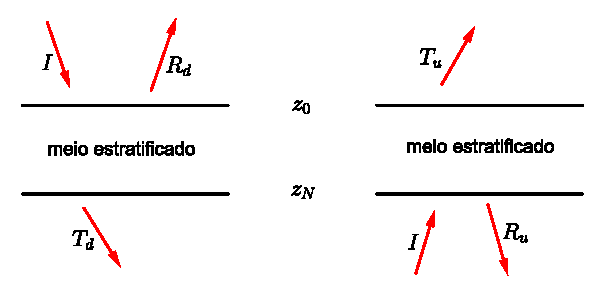
\includegraphics[scale=1.6]{ondas_ascen_descen}
%\caption{\textit{Dire\c{c}\~ao e sentido de propaga\c{c}\~ao de ondas ascendentes e descendentes em camadas homog\^eneas.}}
%\label{fig.ondas_ascen_descen}
%\end{figure}
%Vamos usar a const\^ancia da fun\c{c}\~ao dada na equa\c{c}\~ao \ref{eq.G(V,W)} para igualar seus valores calculados no topo e no fundo da pilha de camadas. Mas aqui, vamos tomar as ondas $V$ e $W$ com for\c{c}a $I$ em sentido descendente e ascendente, respectivamente.  
%\begin{equation*}
%\begin{bmatrix}
%R_d^\top&I
%\end{bmatrix}
%\begin{bmatrix}
%0&I\\
%-I&0
%\end{bmatrix}
%\begin{bmatrix}
%T_u\\
%0
%\end{bmatrix}
%=
%\begin{bmatrix}
%0&T_d^\top
%\end{bmatrix}
%\begin{bmatrix}
%0&I\\
%-I&0
%\end{bmatrix}
%\begin{bmatrix}
%I\\
%R_u
%\end{bmatrix}\,,
%\end{equation*}
%de onde conclu\'imos que
%\begin{equation}\label{eq.T}
%T_u=T_d^\top\,.
%\end{equation}
%Podemos ainda calcular o valor da fun\c{c}\~ao usando somente ondas descendentes $G(V,V)$. Igualando seus valores para o topo e a base da pilha de camadas, temos
%\begin{equation*}
%\begin{bmatrix}
%R_d^\top&I
%\end{bmatrix}
%\begin{bmatrix}
%0&I\\
%-I&0
%\end{bmatrix}
%\begin{bmatrix}
%R_d\\
%0
%\end{bmatrix}
%=
%\begin{bmatrix}
%0&R_d^\top
%\end{bmatrix}
%\begin{bmatrix}
%0&I\\
%-I&0
%\end{bmatrix}
%\begin{bmatrix}
%I\\
%R_d
%\end{bmatrix}\,,
%\end{equation*}
%de onde conclu\'imos que 
%\begin{equation}\label{eq.R_d}
%R_d=R_d^\top\,.
%\end{equation}
%Analogamente, para ondas ascendentes $G(W,W)$, temos \begin{equation}\label{eq.R_u}
%R_u=R_u^\top\,.
%\end{equation}
%Utilizando as equa\c{c}\~oes \ref{eq.T}, \ref{eq.R_d} e \ref{eq.R_u}, podemos definir uma matriz $R$ onde as componentes representam todas as ondas refletidas e transmitidas,
%\begin{equation*}
%R=
%\begin{bmatrix}
%R_d&T_u\\
%T_d&R_u
%\end{bmatrix}\,,
%\end{equation*}
%e verificar que 
%\begin{equation*}
%R=R^\top\,.
%\end{equation*}
%A matriz $R$ est\'a relacionada \`a matriz $S$ usada em \textit{Teoria de Dispers\~ao} de ondas,
%\begin{equation*}
%S=
%\begin{bmatrix}
%T_d&R_u\\
%R_d&T_u
%\end{bmatrix}\,,
%\end{equation*}
%e a matriz $S$ relaciona, de forma linear, ondas saindo de uma pilha de camadas com ondas entrando na pilha,
%\begin{equation*}
%\begin{bmatrix}
%\mathbf{D}(z_N)\\
%\mathbf{U}(z_0)
%\end{bmatrix}
%=
%S(z_0,z_N)\,
%\begin{bmatrix}
%\mathbf{D}(z_0)\\
%\mathbf{U}(z_N)
%\end{bmatrix}\,.
%\end{equation*} 
%
%\subsection{Rela\c{c}\~ao das Matrizes de Transmiss\~ao e Reflex\~ao com a matriz de Propaga\c{c}\~ao}
%
%As matrizes de reflex\~ao e transmiss\~ao podem ser escritas em termos das submatrizes da matriz de propaga\c{c}\~ao, da seguinte forma:
%\begin{align}\nonumber
%T_u(z_0,z_N)&=Q_{11}^{-1}(z_N,z_0)\,,\\\nonumber
%R_u(z_0,z_N)&=Q_{21}(z_N,z_0)\,Q_{11}^{-1}(z_N,z_0)\,,\\\label{eq.relacao_Q_R_T}
%R_d(z_0,z_N)&=-Q_{11}^{-1}(z_N,z_0)\,Q_{12}(z_N,z_0)\,,\\\nonumber
%T_d(z_0,z_N)&=Q_{22}(z_N,z_0)-Q_{21}(z_N,z_0)\,Q_{11}^{-1}(z_N,z_0)\,Q_{12}(z_N,z_0)\,,
%\end{align}
%e a matriz de propaga\c{c}\~ao \'e dada em fun\c{c}\~ao das matrizes de reflex\~ao e transmiss\~ao por
%\begin{equation*}
%Q(z_0,z_N)=
%\begin{bmatrix}
%T_u^{-1}&-T_u^{-1}R_d\\
%R_uT_u^{-1}&T_d-R_uT_u^{-1}R_d
%\end{bmatrix}\,.
%\end{equation*}
%
%
%Para o caso de camadas homog\^eneas, usando as equa\c{c}\~oes \ref{eq.Q(z,z_0)} e \ref{eq.relacao_Q_R_T}, podemos deduzir que, para matrizes de transmiss\~ao,
%\begin{equation*}
%T_d(z_0,z)=T_u(z_0,z)=\exp\left[\pm i\omega\,\Lambda(z-z_0)\right]\,,
%\end{equation*}
%e para matrizes de reflex\~ao
%\begin{equation*}
%R_d(z_0,z)=R_u(z_0,z)=0\,.
%\end{equation*}
%
%Vamos definir $E_{k+1}(-\pm i\omega)=\exp\left[-\pm i\omega\,\Lambda(z_{k+1}-z_k)\right]$. Assim, a matriz $S$ para uma camada homog\^enea e para interface para a pr\'oxima camada \'e dada pelo \textit{produto estrela},
%\begin{align*}
%S(z_{k+},z_{k+1+})&=S(z_{k+},z_{k+1-})*S(z_{k+1-},z_{k+1+})\\\\
%&=
%\begin{bmatrix}
%E_{k+1}(-\pm i\omega)&0\\
%0&E_{k+1}(-\pm i\omega)
%\end{bmatrix}
%*
%\begin{bmatrix}
%T_{d,k+1}&R_{u,k+1}\\
%R_{d,k+1}&T_{u,k+1}
%\end{bmatrix}\\\\
%&=
%\begin{bmatrix}
%T_{d,k+1}E_{k+1}(-\pm i\omega)&R_{u,k+1}\\
%E_{k+1}(-\pm i\omega)R_{d,k+1}E_{k+1}(-\pm i\omega)&E_{k+1}(-\pm i\omega)T_{u,k+1}
%\end{bmatrix}\,.
%\end{align*}
\chapter{Conclus\~oes e Trabalhos Futuros}
Neste trabalho apresentamos um tratamento matem\'atico das EDP's do efeito magneto-el\'astico encontrado em \cite{pinho_2018} , no sentido de propiciar a contru\c{c}\~ao de um algoritmo num\'erico est\'avel que possa descrever a propaga\c{c}\~ao acoplada de ondas el\'asticas e eletromagn\'eticas. Nesse tratamento foi fundamental a aplica\c{c}\~ao de conhecimentos da F\'isica-Matem\'atica, Geof\'isica e, em particular, um metodo matricial que facilita a an\'alise de propaga\c{c}\~ao de ondas em meios estratificados.

Vimos na subse\c{c}\~ao \ref{sec.matricial_poroelast} a possibilidade de an\'alise de dispers\~ao de atenua\c{c}\~ao de ondas para casos diversos, onde tal an\'alise auxilia na verifica\c{c}\~ao e constru\c{c}\~ao de um c\'odigo computacional efetivo para descrever a propaga\c{c}\~ao dessas ondas. Numa oportuinidade futura, queremos aplicar a an\'alise de atenua\c{c}\~ao e dispers\~ao nesse sistema de EDP's do efeito magneto-el\'astico com a finalidade de ajudar a estudar o comportamento da propaga\c{c}\~ao.

Numa determinada abordagem, a an\'alise de casos mais simples auxilia no estudo de casos mais sofisticados. Por tanto, no intuito ainda de otimizar o estudo da propaga\c{c}\~ao das ondas, faremos o tratamento matem\'atico das EDP's de magneto-elasticidade para o caso unidimensional, considerando a propaga\c{c}\~ao em fun\c{c}\~ao do tempo e em fun\c{c}\~ao da profundidade. Neste caso podemos utilizar o m\'etodo matricial e a an\'alise de atenua\c{c}\~ao e dispers\~ao das ondas, e economizamos a utiliza\c{c}\~ao de transformadas e mudan\c{c}a de eixos coordenados.

O formato final das EDO's dado no cap\'itulo \ref{sec.trans_edp_2_edo} apresentou algumas vari\'aveis incluidas como fonte, diferentemente do que \'e preconizado por Ursin, onde todas a vari\'aveis devem estar inseridas no vetor $\mathbf{\Phi}$. Assim, analisaremos a possibilidade da aplica\c{c}\~ao de fun\c{c}\~oes de Green juntamente com o m\'etodo matricial para contornar esse problema. \'E poss\'ivel que essa abordagem traga desafios computacionais consider\'aveis e da\'i estudaremos tamb\'em outras alternativas. Uma delas \'e considerar o efeito magento-el\'astico para o caso totalmente acoplado e verificar se o novo formato das equa\c{c}\~oes permite a exclus\~ao de vari\'avies dadas como fonte. Outra possibilidade \'e escrever as equa\c{c}\~oes em coordenadas cil\'indricas, considerar as propriedades de isotropia das camadas e substituir as coordenadas horizontais somente pelo raio.

A implementa\c{c}\~ao do algoritmo computacional ser\'a realizada em linguagem C++, por conta de algumas caracter\'isticas apresentadas por esta linguagem descritas em \cite{bueno_2015}, como: ser de prop\'osito geral podendo ser utilizada na constru\c{c}\~ao de programas computacionais, aplicativos de sistemas embarcados e em computa\c{c}\~ao cient\'ifica; ser de alto n\'ivel e orientada a objeto, permitindo a propagama\c{c}\~ao simult\^anea realizada por v\'arios programadores trabalhando num mesmo projeto; fortemente tipada o que ajuda na detec\c{c}\~ao de \textit{bugs} e controle e gerenciamento de mem\'oria; ser a mais utilizada em sistemas complexos e grandes no uso de programa\c{c}\~ao paralela.

\bibliographystyle{plainnat}
%\bibliography{referencias}

\begin{thebibliography}{25}
\providecommand{\natexlab}[1]{#1}
\providecommand{\url}[1]{\texttt{#1}}
\expandafter\ifx\csname urlstyle\endcsname\relax
  \providecommand{\doi}[1]{doi: #1}\else
  \providecommand{\doi}{doi: \begingroup \urlstyle{rm}\Url}\fi

\bibitem[Azeredo(2013)]{Azeredo_2013}
M.~M. Azeredo.
\newblock \emph{Modelagem Matem\'atica e Computacional da Propaga\c{c}\~ao de
  Ondas S\'ismicas em Meios Poroel\'asticos Estratificados}.
\newblock PhD thesis, Universidade Estadual do Norte Fluminense, 2013.

\bibitem[Baruch(2013)]{baruch_2013}
E.~M. Baruch.
\newblock The classical hankel transform in the kirillov model of discrete
  series.
\newblock \emph{Integral Transforms and Special Functions}, 24, 2013.
%\newblock \doi{10.1080/10652469.2012.691097}.

\bibitem[Bueno(2015)]{bueno_2015}
A.~D. Bueno.
\newblock \emph{Programa\c{c}\~ao Orientada a Objeto com C++}.
\newblock Novatec, 2015.

\bibitem[Butkov(1988)]{butkov_88}
E.~Butkov.
\newblock \emph{F\'isica Matem\'atica}.
\newblock LTC, 1988.

\bibitem[Chew(1995)]{chew}
W.~C. Chew.
\newblock \emph{Waves and Fields in Inhomogeneous Media}.
\newblock IEEE PRESS, 1995.

\bibitem[Dunkin and Eringen(1963)]{eringen_1963}
J.W. Dunkin and A.C. Eringen.
\newblock On the propagation of waves in an electromagnetic elastic solid.
\newblock \emph{International Journal of Engineering Science}, 1, 1963.

\bibitem[Savit(1988)]{dobrin_88}
M.~B.~Dobrin e~C.~H.~Savit.
\newblock \emph{Introduction to Geophysical Prospecting}.
\newblock McGraw-Hill, 1988.

\bibitem[Farlow(1993)]{farlow_93}
S.~J. Farlow.
\newblock \emph{Partial Differential Equations for Scientists and Engineers}.
\newblock Dover, 1993.

\bibitem[Fatianov and Mikhailenko(1989)]{Mikhailenko_89}
A.G. Fatianov and B.G. Mikhailenko.
\newblock Numerically-analytical method for calculation of theoretical
  seismograms in layered-inhomogeneous anelastic media.
\newblock \emph{In Proceedings of the 7 th International Mathematical
  Geophysics Seminar held at the Free University of Berlin}, 1989.

\bibitem[Griffiths(1999)]{griffiths}
D.~J. Griffiths.
\newblock \emph{Introduction to Electrodynamics}.
\newblock Prentice-Hall, 1999.

\bibitem[Lang(1986)]{lang_1986}
S.~Lang.
\newblock \emph{Introduction to Linear Algebra}.
\newblock Springer, 1986.

\bibitem[Lebedev and Cloud(2003)]{lebedev_2003}
L.~P. Lebedev and M.~J. Cloud.
\newblock \emph{Tensor Analysis}.
\newblock World Scientific Publishing, 2003.

\bibitem[Mikhailenko and Soboleva(1997)]{mikhailenko_97}
B.~G. Mikhailenko and O.~N. Soboleva.
\newblock Mathematical modeling of seismomagnetic efects arising in the seismic
  wave motion in the earth's constant magnetic field.
\newblock \emph{Appl. Math. Lett.}, 10\penalty0 (3):\penalty0 47--51, 1997.

\bibitem[Miranda(2016)]{miranda_2016}
M.~R. S.~T. Miranda.
\newblock \emph{M\'etodo Matricial em Modelagem Poroel\'astica: Modelo de
  Biot-JKD}.
\newblock UENF, 2016.

\bibitem[Novacki(1983)]{Novacki_83}
W.~Novacki.
\newblock Electromagnetic efects in solid bodies.
\newblock \emph{In Panstwowe Wydawnictwo Naukowe}, 10, 1983.

\bibitem[Oliveira(2018)]{oliveira_2018}
I.~B. Oliveira.
\newblock \emph{Modelagem de Propaga\c{c}\~ao das Ondas El\'asticas em Meios
  Porosos 1D: Modelo de Biot vs. Biot-JKD}.
\newblock UENF, 2018.

\bibitem[Pinho(2018)]{pinho_2018}
D.~C. Pinho.
\newblock \emph{Fundamentos de Magneto-Elasticidade}.
\newblock UENF, 2018.

\bibitem[Pride(1994)]{pride_94}
S.~Pride.
\newblock Governing equations for the coupled electromagnetics and acustics of
  porous media.
\newblock \emph{Physical Review B}, 1994.

\bibitem[Ursin(1983)]{Ursin-1983}
B.~Ursin.
\newblock Review of elastic and electromagnetic wave propagation in
  horizontally layered media.
\newblock \emph{The Leading Edge}, 48, 08 1983.

\bibitem[Weyl(1919)]{weyl_19}
H.~Weyl.
\newblock Ausbreitung elektromagnetischen wellen ueber einem ebenen leiter.
\newblock \emph{Annalen der Physik}, 1919.

\bibitem[White and Zhou(2006)]{White_Zhou_2006}
B.S. White and M.~Zhou.
\newblock Eletroseismic prospecting in layered media.
\newblock \emph{Society for Industrial and Applied Mathematics}, 67\penalty0
  (1):\penalty0 69--98, 2006.

\end{thebibliography}

\end{document}